% Template luận văn cho SV trường ĐHKHTN
% Liên hệ: nqminh@fit.hcmus.edu.vn
% Last update: 11/08/2015

% LƯU Ý: Để phần tài liệu tham khảo hiển thị đúng, cần phải build clean (xoá các file build cũ), sau khi build file BIB cần build lại file TEX 2 lần.
% Phần in tài liệu tham khảo: phải gán lại resetnumbers=số tài liệu tham khảo tiếng Việt + 1 (dòng 101 file này)

%\documentclass[oneside,a4paper,13pt]{extreport}
\documentclass[oneside,a4paper,13pt]{extreport}
%
\usepackage{titlesec}
\usepackage[absolute,overlay]{textpos}

% Định dạng tiêu đề \chapter
\titleformat{\chapter}[hang]{\normalfont\Large\bfseries}{CHƯƠNG \thechapter.}{2pc}{}
% Định dạng tiêu đề \section
\titleformat{\section}[hang]{\normalfont\Large\bfseries}{\thesection}{1em}{}
% Định dạng tiêu đề \subsection
\titleformat{\subsection}[hang]{\normalfont\large\bfseries}{\thesubsection}{1em}{}

% Font tiếng Việt
\usepackage[T5]{fontenc}
\usepackage[utf8]{inputenc}
\DeclareTextSymbolDefault{\DH}{T1} % Ký tự mã \DH == Đ
%To remove warning Font shape OT1/cmr/m/n' in size <13> not available(Font) size <12> substituted
\usepackage{lmodern} 

%\usepackage[vietnamese]{babel} % Tự động thay đổi Chapter -> Chương...
% Màu chữ
\usepackage{xcolor}
%Comments (Cần dùng chung với gói xcolor)
\newcommand\comment[1]{{\color{blue}\textit{#1}}}



% Tài liệu tham khảo
\usepackage[
	sorting=nty,
	backend=biber,
	defernumbers=true]{biblatex}
%
\usepackage{setspace}
\usepackage[unicode]{hyperref} % Bookmark tiếng Việt
\addbibresource{References/references.bib}
%glossaries
%\usepackage[automake]{glossaries}
\usepackage[automake,style=altlist]{glossaries}  % Đặt lệnh này trong preamble
%\usepackage[style=altlist,toc=true]{glossaries}
\makeglossaries % Đừng quên lệnh này để tạo danh mục

\label{glossary}

%backbone
\newglossaryentry{backbone}{
	name={backbone},
	description={Hay còn gọi \textit{mạng xương sống} trong tiếng Việt, là phần cơ bản của mô hình chịu trách nhiệm trích xuất các đặc trưng từ dữ liệu đầu vào. Các cấu trúc phổ biến thường sử dụng làm \textit{backbone} trong các nhiệm vụ liên quan đến hình ảnh gồm ResNet, VGG, và EfficientNet},
	short={backbone},
}
%
%up-sampling 
\newglossaryentry{up-sampling}{
	name={up-sampling},
	description={Toán tử \textit{up-sampling} có chức năng tăng kích thước của ảnh bằng cách chèn các điểm mới giữa các điểm hiện có, được dùng phổ biến trong các mô hình tạo sinh, nhằm tăng kích thước của đầu ra so với đầu vào},
	short={up-sampling},
}

%convolution
\newglossaryentry{convolution}{
	name={convolution},
	description={Toán tử \textit{convolution}~\cite{convolution} là một toán tử được sử dụng trong mạng tích chập, dùng để trích xuất đặc trưng của tín hiệu},
	short={convolution},
}

%histogram
\newglossaryentry{histogram}{
	name={histogram},
	description={Là một biểu đồ cột biểu diễn sự phân bố các giá trị màu sắc hoặc mức xám trong một hình ảnh. Biểu đồ này cung cấp một cái nhìn tổng quan về tần suất xuất hiện của các giá trị màu sắc khác nhau trong ảnh, từ đó có thể hiểu rõ hơn về đặc điểm của ảnh, chẳng hạn như độ sáng, độ tương phản, và sự cân bằng màu.
	 },
	short={histogram},
}

%bilinear
\newglossaryentry{bilinear}{
	name={bilinear},
	description={Hay gọi đầy đủ là \textit{Bilinear interpolation}  \cite{mastylo2013bilinear}- Nội suy song tuyến tính, là phương pháp được sử dụng phổ biến để phóng to hoặc thu nhỏ ảnh. Giá trị của điểm ảnh mới được tính toán dựa trên trung bình trọng số của 4 điểm ảnh lân cận theo cả trục ngang ($x$) và dọc ($y$).},
	short={bilinear},
}


\newglossaryentry{epoch}{
	name={epoch},
	description={Một vòng lặp hoàn chỉnh qua toàn bộ tập dữ liệu huấn luyện. Trong một \textit{epoch}, mô hình được cập nhật nhiều lần, mỗi lần với một batch dữ liệu},
	short={epoch}
}

\newglossaryentry{batch}{
	name={batch},
	description={Là một tập con của dữ liệu huấn luyện được sử dụng trong một lần lan truyền tiến và lan truyền ngược trong quá trình huấn luyện. Việc chia dữ liệu thành các batch giúp tối ưu hóa bộ nhớ và tăng tốc quá trình huấn luyện thông qua tính toán song song},
	short={batch},
}

\newglossaryentry{overfitting}{
	name={overfitting},
	description={Là hiện tượng xảy ra khi mô hình học quá kỹ các chi tiết và nhiễu trong tập huấn luyện, dẫn đến hiệu suất kém khi áp dụng cho dữ liệu chưa từng thấy. Mô hình bị \textit{overfitting} sẽ có sai số huấn luyện thấp nhưng sai số kiểm tra cao},
	short={overfitting},
}

\newglossaryentry{adam}{
	name={adam},
	description={Thuật toán tối ưu phổ biến trong huấn luyện mạng nơ-ron, kết hợp giữa momentum và điều chỉnh tốc độ học theo từng tham số. Tên đầy đủ là Adaptive Moment Estimation},
	short={adam},
}

\newglossaryentry{cnn}{
	name={CNN},
	description={Mạng nơ-ron tích chập, thường được dùng trong các bài toán xử lý ảnh và nhận dạng mẫu. CNN sử dụng các lớp tích chập để tự động học các đặc trưng không gian từ dữ liệu ảnh đầu vào.},
	first={Convolutional Neural Network (CNN)},
	plural={CNNs}
}

\newglossaryentry{skipconnection}{
	name={skip connection},
	description={Kết nối bỏ qua; kỹ thuật kết nối đầu vào của một lớp với đầu ra của lớp sâu hơn, thường dùng trong mạng sâu như ResNet để giảm hiện tượng mất mát thông tin và giúp gradient lan truyền dễ dàng hơn.}
}


\newglossaryentry{fft}{
	name={FFT},
	description={viết tắt của \textit{Fast Fourier Transform}, tức Biến đổi Fourier nhanh. Đây là thuật toán hiệu quả để chuyển đổi tín hiệu từ miền thời gian sang miền tần số, thường được dùng trong xử lý tín hiệu và phân tích ảnh},
	first={biến đổi Fourier nhanh (FFT)},
	plural={FFTs}
}

\newglossaryentry{ifft}{
	name={iFFT},
	description={viết tắt của \textit{Inverse Fast Fourier Transform}, tức Biến đổi Fourier ngược nhanh. Đây là thuật toán dùng để chuyển tín hiệu từ miền tần số trở về miền thời gian},
	first={biến đổi Fourier ngược nhanh (iFFT)},
	plural={iFFTs}
}

\newglossaryentry{dft}{
	name={DFT},
	description={viết tắt của \textit{Discrete Fourier Transform}, tức Biến đổi Fourier rời rạc. Đây là phép biến đổi dùng để phân tích một tín hiệu rời rạc theo miền tần số},
	first={biến đổi Fourier rời rạc (DFT)},
	plural={DFTs}
}

\newglossaryentry{gpu}{
	name={GPU},
	description={viết tắt của \textit{Graphics Processing Unit}, tức bộ xử lý đồ họa. GPU có khả năng xử lý song song cao, thường được dùng để tăng tốc quá trình huấn luyện mạng học sâu},
	first={GPU},
	plural={GPUs}
}

\newglossaryentry{deepfake}{
	name={deepfake},
	description={là từ ghép giữa “deep learning” (học sâu) và “fake” (giả mạo). Deepfake là nội dung đa phương tiện (ảnh, video, âm thanh) được tạo ra bằng các kỹ thuật học sâu, khiến chúng trông như thật nhưng thực tế là giả mạo},
	first={deepfake},
	plural={deepfakes}
}

\newglossaryentry{bce}{
	name={binary cross-entropy},
	description={là một hàm mất mát được dùng phổ biến trong các bài toán phân lớp nhị phân, giúp đo lường sự khác biệt giữa xác suất dự đoán và nhãn thực tế},
	first={binary cross-entropy},
	plural={}
}

\newglossaryentry{knowledgedistillation}{
	name={knowledge distillation},
	description={là kỹ thuật huấn luyện mô hình nhỏ hơn (student) bằng cách học từ mô hình lớn hơn (teacher), thông qua đầu ra hoặc biểu diễn đặc trưng trung gian},
	first={knowledge distillation},
	plural={}
}

\newglossaryentry{fbkd}{
	name={feature-based knowledge distillation},
	description={là một kỹ thuật trong huấn luyện mạng học sâu, trong đó một mô hình nhỏ hơn (student) học từ mô hình lớn hơn (teacher) thông qua đặc trưng trung gian (feature), thay vì chỉ học từ đầu ra cuối cùng},
	first={rút trích tri thức dựa trên đặc trưng (Feature-Based Knowledge Distillation)},
	plural={Feature-Based Knowledge Distillation}
}

\newglossaryentry{distillation}{
	name={distillation},
	description={trong lĩnh vực học sâu, distillation (rút trích tri thức) là kỹ thuật huấn luyện một mô hình nhỏ (student) bằng cách học theo hành vi hoặc biểu diễn của một mô hình lớn đã được huấn luyện trước (teacher)},
	first={distillation},
	plural={}
}

\newglossaryentry{stride}{
	name={stride},
	description={là một tham số trong lớp tích chập (convolution) hoặc pooling, biểu thị số bước mà cửa sổ trượt di chuyển trên ảnh đầu vào. Stride càng lớn thì kích thước đầu ra càng nhỏ},
	first={stride},
	plural={}
}

\newglossaryentry{padding}{
	name={padding},
	description={là kỹ thuật thêm các giá trị (thường là 0) xung quanh biên của ảnh đầu vào trong mạng tích chập. Mục đích là để giữ nguyên kích thước không gian đầu ra hoặc kiểm soát kích thước khi thực hiện phép tích chập},
	first={padding},
	plural={}
}

\newglossaryentry{relu}{
	name={ReLU},
	description={viết tắt của \textit{Rectified Linear Unit}, là một hàm kích hoạt trong mạng nơ-ron, được định nghĩa là \( f(x) = \max(0, x) \). ReLU giúp mô hình học phi tuyến và có khả năng lan truyền gradient hiệu quả hơn},
	first={ReLU (Rectified Linear Unit)},
	plural={}
}

\newglossaryentry{kernel}{
	name={kernel},
	description={trong mạng nơ-ron tích chập, kernel (hay còn gọi là filter) là một ma trận trọng số nhỏ dùng để quét qua ảnh đầu vào và trích xuất các đặc trưng như biên, góc cạnh, họa tiết,...},
	first={kernel},
	plural={kernels}
}

\newglossaryentry{maxpooling}{
	name={max pooling},
	description={là một phép toán trong mạng nơ-ron tích chập dùng để giảm kích thước đầu ra bằng cách lấy giá trị lớn nhất trong mỗi vùng nhỏ của ảnh đặc trưng. Max Pooling giúp giảm số lượng tham số và tăng tính khái quát của mô hình},
	first={max pooling},
	plural={}
}

\newglossaryentry{gap}{
	name={global average pooling},
	description={là một kỹ thuật trong mạng nơ-ron tích chập, thay vì dùng các lớp fully connected, GAP tính trung bình toàn bộ mỗi bản đồ đặc trưng (feature map) và tạo ra một đầu ra duy nhất cho mỗi kênh. Phương pháp này giúp giảm số lượng tham số và hạn chế overfitting},
	first={global average pooling},
	plural={}
}

\newglossaryentry{fc}{
	name={fully connected layer},
	description={là lớp trong mạng nơ-ron trong đó mỗi đầu vào được kết nối với tất cả các nút ở lớp tiếp theo. Lớp này thường xuất hiện ở cuối mô hình để đưa ra quyết định phân loại},
	first={fully connected layer},
	plural={}
}

\newglossaryentry{sigmoid}{
	name={sigmoid},
	description={là một hàm kích hoạt trong mạng nơ-ron, được định nghĩa là \( \sigma(x) = \frac{1}{1 + e^{-x}} \). Hàm sigmoid đưa đầu ra về khoảng (0, 1), thích hợp cho các bài toán phân lớp nhị phân},
	first={sigmoid},
	plural={}
}

\newglossaryentry{generator}{
	name={generator},
	description={trong mô hình GAN, generator là mạng học sâu có nhiệm vụ sinh ra dữ liệu giả sao cho giống dữ liệu thật nhất có thể, nhằm đánh lừa discriminator},
	first={generator (mạng sinh dữ liệu giả)},
	plural={generators}
}

\newglossaryentry{discriminator}{
	name={discriminator},
	description={trong mô hình GAN, discriminator là mạng học sâu có nhiệm vụ phân biệt dữ liệu thật và dữ liệu do generator tạo ra},
	first={discriminator (mạng phân biệt thật – giả)},
	plural={discriminators}
}

\newglossaryentry{gaussian}{
	name={gaussian},
	description={là một phân phối xác suất liên tục có dạng hình chuông đối xứng, còn gọi là phân phối chuẩn (normal distribution), được sử dụng rộng rãi trong thống kê và học máy để mô hình hóa dữ liệu nhiễu hoặc phân bố tự nhiên},
	first={gaussian},
	plural={}
}

\newglossaryentry{grayscale}{
	name={gray-scale},
	description={là dạng ảnh chỉ bao gồm các mức độ xám, mỗi điểm ảnh được biểu diễn bằng một giá trị cường độ ánh sáng, thường từ 0 (đen) đến 255 (trắng)},
	first={gray-scale},
	plural={}
}

\newglossaryentry{texture}{
	name={texture},
	description={thuật ngữ trong xử lý ảnh biểu thị các mẫu lặp lại hoặc sự thay đổi cường độ ánh sáng, màu sắc trên bề mặt hình ảnh, dùng để mô tả độ mịn, nhám hoặc cấu trúc vật liệu},
	first=kết cấu bề mặt (texture),
	plural={textures}
}

\newglossaryentry{poortexteregion}{
	name={poor texture regions},
	description={các vùng ảnh có rất ít thông tin kết cấu, bề mặt tương đối đồng đều và ít thay đổi về cường độ, khiến việc phát hiện đặc trưng trở nên khó khăn},
	first={vùng kết cấu đơn giản (poor texture regions)},
	plural={}
}

\newglossaryentry{richtexteregion}{
	name={rich texture regions},
	description={các vùng ảnh chứa nhiều thông tin kết cấu, có sự thay đổi rõ rệt về cường độ hoặc hoa văn, giúp trích xuất đặc trưng dễ dàng hơn},
	first={vùng kết cấu phức tạp (rich texture regions)},
	plural={}
}

\newglossaryentry{patch}{
	name={patch},
	description={một vùng nhỏ hình vuông hoặc hình chữ nhật được trích xuất từ hình ảnh gốc, thường được sử dụng để phân tích cục bộ hoặc huấn luyện mô hình học sâu},
	first={mảnh ảnh nhỏ (patch)},
	plural={patches}
}

\newglossaryentry{azimuthalaveraging}{
	name={azimuthal averaging},
	description={kỹ thuật tính trung bình các giá trị theo hướng góc (azimuth) trong hệ tọa độ cực, thường được áp dụng trên ảnh hoặc phổ tần số để rút gọn dữ liệu thành một hàm một chiều theo bán kính},
	first={trung bình theo phương góc (azimuthal averaging)},
	plural={}
}

\newglossaryentry{svm}{
	name={SVM},
	description={là một thuật toán học có giám sát được sử dụng để phân loại và hồi quy, hoạt động bằng cách tìm siêu phẳng tối ưu phân tách các lớp dữ liệu khác nhau},
	first={Support Vector Machine (SVM)},
	plural={}
}

\newglossaryentry{kmeans}{
	name={K-means},
	description={là thuật toán phân cụm không có giám sát, chia dữ liệu thành $K$ nhóm sao cho khoảng cách nội nhóm được tối thiểu hoá. Thuật toán hoạt động bằng cách cập nhật các tâm cụm và gán lại nhãn lặp đi lặp lại cho đến khi hội tụ},
	first={K-means},
	plural={}
}

\newglossaryentry{logisticregression}{
	name={Logistic Regression},
	description={là một mô hình học có giám sát dùng để giải bài toán phân loại nhị phân, dựa trên hàm sigmoid để ánh xạ đầu ra về khoảng xác suất $[0, 1]$},
	first={hồi quy logistic (Logistic Regression)},
	plural={}
}

\newglossaryentry{dct}{
	name={DCT},
	description={là một phép biến đổi tương tự như biến đổi Fourier, dùng để biểu diễn tín hiệu dưới dạng tổ hợp các hàm cosine với tần số khác nhau. DCT thường được sử dụng trong nén ảnh và xử lý tín hiệu do khả năng tập trung năng lượng tốt},
	first={biến đổi Cosine rời rạc (Discrete Cosine Transform – DCT)},
	plural={}
}

\newglossaryentry{nearestneighbor}{
	name={nearest neighbor},
	description={là phương pháp nội suy đơn giản trong xử lý ảnh, trong đó mỗi điểm mới được gán giá trị của điểm lân cận gần nhất. Phương pháp này rất nhanh nhưng có thể tạo ra ảnh bậc thang và thiếu mượt mà},
	first={phương pháp láng giềng gần nhất (nearest neighbor)},
	plural={}
}


\newglossaryentry{binomial}{
	name={binomial filter},
	description={là bộ lọc làm mượt hình ảnh dựa trên hệ số nhị thức Pascal. Trong nội suy, binomial filter giúp làm trơn dữ liệu đầu ra bằng cách sử dụng các trọng số giống Gaussian một cách đơn giản},
	first={bộ lọc nhị thức (binomial filter)},
	plural={}
}

\newglossaryentry{binomialupsampling}{
	name={binomial up-sampling},
	description={là kỹ thuật phóng to ảnh bằng cách chèn thêm điểm ảnh (zero-insertion) và sau đó làm mượt bằng bộ lọc nhị thức (binomial filter). Phương pháp này giúp giảm hiện tượng răng cưa và tạo ảnh mượt mà hơn so với nội suy đơn giản},
	first={nội suy nhị thức (binomial up-sampling)},
	plural={}
}

\newglossaryentry{optimizer}{
	name={optimizer},
	description={là thuật toán tối ưu dùng trong huấn luyện mạng học sâu, nhằm cập nhật các tham số mô hình để giảm hàm mất mát. Một số thuật toán tối ưu phổ biến gồm SGD, Adam, RMSProp},
	first={optimizer},
	plural={}
}

\newglossaryentry{learningrate}{
	name={learning rate},
	description={là siêu tham số quyết định bước nhảy trong quá trình cập nhật tham số mô hình. Giá trị learning rate quá lớn có thể gây dao động, còn quá nhỏ khiến quá trình huấn luyện chậm},
	first={learning rate},
	plural={}
}

\newglossaryentry{batchsize}{
	name={batch size},
	description={là số lượng mẫu được sử dụng trong mỗi lần cập nhật tham số trong quá trình huấn luyện. Batch size ảnh hưởng đến tốc độ huấn luyện, bộ nhớ và độ ổn định của mô hình},
	first={batch size},
	plural={}
}

\newglossaryentry{pytorch}{
	name={PyTorch},
	description={là một thư viện mã nguồn mở chuyên dùng để xây dựng và huấn luyện các mô hình học sâu, hỗ trợ linh hoạt cả nghiên cứu và triển khai thực tế, phát triển bởi Facebook AI Research},
	first={PyTorch},
	plural={}
}

\newglossaryentry{batchnorm}{
	name={batch normalization},
	description={Kỹ thuật chuẩn hoá dữ liệu đầu vào của từng lớp trong mạng nơ-ron bằng cách đưa chúng về phân phối chuẩn (zero mean, unit variance) trong mỗi mini-batch, giúp tăng tốc quá trình huấn luyện và cải thiện độ ổn định của mô hình}
}

\newglossaryentry{bottleneck}{
	name=bottleneck,
	description={Một khối trong kiến trúc ResNet gồm ba lớp convolution liên tiếp (1×1, 3×3, 1×1), giúp giảm chi phí tính toán mà vẫn giữ được khả năng học đặc trưng}
}

\newglossaryentry{mse}{
	name={MSE},
	description={là viết tắt của \textit{Mean Squared Error}, một hàm mất mát phổ biến dùng để đo sai số bình phương trung bình giữa đầu ra dự đoán và nhãn thật trong các mô hình học máy},
	first={Mean Squared Error (MSE)},
	plural={}
}

\newglossaryentry{teacher}{
	name={teacher},
	description={Mô hình được huấn luyện trước, đóng vai trò truyền đạt tri thức cho mô hình Student thông qua cơ chế lan truyền tri thức (Knowledge Distillation)},
	plural={}
}

\newglossaryentry{student}{
	name={student},
	description={Mô hình nhẹ hơn, được huấn luyện bằng cách học theo đầu ra của mô hình Teacher thông qua lan truyền tri thức},
	plural={}
}

\newglossaryentry{layer}{
	name={layer},
	description={là một tầng trong mạng nơ-ron, thực hiện một phép biến đổi dữ liệu đầu vào thành đầu ra. Các loại layer phổ biến gồm convolutional layer, pooling layer và fully connected layer},
	first={layer},
	plural={layers}
}

\newglossaryentry{attention}{
	name={attention},
	description={là cơ chế giúp mô hình học sâu tập trung vào các phần thông tin quan trọng hơn trong chuỗi đầu vào, được sử dụng phổ biến trong mô hình Transformer và các biến thể của nó},
	first={attention},
	plural={}
}

\newglossaryentry{classification}{
	name={classification},
	description={là một dạng bài toán trong học máy, trong đó mô hình học cách phân loại đầu vào vào các nhóm hoặc lớp đã biết. Các loại phân loại gồm phân loại nhị phân, phân loại đa lớp, v.v.},
	first={classification},
	plural={}
}

\newglossaryentry{train}{
	name={train},
	description={giai đoạn huấn luyện mô hình, trong đó mô hình học từ tập dữ liệu huấn luyện (training data) để tối ưu hóa các tham số},
	first={train},
	plural={}
}

\newglossaryentry{validation}{
	name={validation},
	description={là quá trình đánh giá mô hình trong quá trình huấn luyện bằng tập dữ liệu riêng biệt, nhằm điều chỉnh siêu tham số và tránh overfitting},
	first={validation},
	plural={}
}

\newglossaryentry{test}{
	name={test},
	description={là giai đoạn kiểm tra hiệu suất mô hình sau khi huấn luyện, sử dụng tập dữ liệu chưa từng thấy để đánh giá khả năng tổng quát hóa},
	first={test},
	plural={}
}

\newglossaryentry{pipeline}{
	name=pipeline,
	description={chuỗi các bước xử lý dữ liệu được tổ chức theo thứ tự nhằm thực hiện một tác vụ nhất định, thường được sử dụng trong học máy, xử lý ảnh, hoặc các hệ thống kỹ thuật số tự động}
}

\newglossaryentry{gradient}{
	name=gradient,
	description={Đạo hàm bậc nhất theo không gian, biểu diễn mức độ và hướng biến thiên cục bộ của tín hiệu hoặc ảnh số}
}

\newglossaryentry{adof}{
	name={ADOF},
	description={Adjacency Difference Orientation Filter - khối tiền xử lý dựa trên bộ lọc thông cao trong miền không gian},
	first={Adjacency Difference Orientation Filter (ADOF)},
	plural={}
}


 % Nhập các định nghĩa từ glossary.tex
% Công thức
\usepackage{amssymb}
% Chèn hình, các hình trong luận văn được để trong thư mục Images/
\usepackage{graphicx}
\graphicspath{{Images/}}
\usepackage{caption}
%\usepackage{subfig}

%Bảng
\usepackage{booktabs}
\usepackage{colortbl}
\usepackage{arydshln}
% Chèn mã nguồn
\usepackage{listings}

% Bảng biểu
\usepackage{multirow}
\usepackage{adjustbox}
\usepackage{tabularray}

% Đổi tên mặc định
\renewcommand{\chaptername}{Chương}
\renewcommand{\figurename}{Hình}
\renewcommand{\tablename}{Bảng}
\renewcommand{\contentsname}{MỤC LỤC}
\renewcommand{\listfigurename}{DANH SÁCH CÁC HÌNH VẼ}
\renewcommand{\listtablename}{DANH SÁCH CÁC BẢNG}
\renewcommand{\appendixname}{PHỤ LỤC}
\renewcommand{\glossaryname}{DANH SÁCH THUẬT NGỮ}
% Dãn dòng 1.5
\usepackage{setspace}
\onehalfspacing

% Canh lề
\usepackage[
  top=35mm,
  bottom=30mm,
  left=35mm,
  right=20mm,
  includefoot]{geometry}
  
% Trang bìa
\usepackage{tikz}
\usetikzlibrary{calc}
\newcommand\HRule{\rule{\textwidth}{1pt}}

\begin{document}

\begin{titlepage}
\begin{tikzpicture}[remember picture, overlay]
  \draw[line width = 2pt] ($(current page.north west) + (2cm,-2cm)$) rectangle ($(current page.south east) + (-1.5cm,2cm)$);
\end{tikzpicture}
\begin{center}
\fontsize{13pt}{20pt}\selectfont
ĐẠI HỌC QUỐC GIA TP. HCM\\
\bfseries TRƯỜNG ĐẠI HỌC KHOA HỌC TỰ NHIÊN\\[4cm]
%
%{ \LARGE \bfseries VÕ HOÀI DANH\\[2cm] } 
\fontsize{14pt}{20pt}\selectfont
{VÕ HOÀI DANH\\[3cm]}
%
%{ \huge \bfseries PHÁT HIỆN HÌNH ẢNH SINH BỞI MÔ HÌNH TẠO SINH ẢNH\\[3cm] } 
\fontsize{16pt}{20pt}\selectfont
{PHÁT HIỆN HÌNH ẢNH \\SINH BỞI MÔ HÌNH TẠO SINH ẢNH \\[3cm]}
%
%\large \textbf{LUẬN VĂN THẠC SĨ}\\[2cm]
\fontsize{14pt}{20pt}\selectfont
{LUẬN VĂN THẠC SĨ}
%
\vfill
\fontsize{12pt}{20pt}\selectfont
\textnormal{Tp. Hồ Chí Minh, Năm 2024}
%
\end{center}
%
\end{titlepage}

\pagenumbering{roman} % Đánh số i, ii, iii, ...

\addcontentsline{toc}{chapter}{LỜI CAM ĐOAN}
\chapter*{
	\begin{center} 
		\fontsize{14pt}{14pt}\selectfont 
		LỜI CAM ĐOAN 
		\end{center}
	}
\label{reassurances}

\fontsize{13pt}{20pt}\selectfont
Tôi xin cam đoan luận văn thạc sĩ ngành Trí tuệ nhân tạo, với đề tài \textbf{Phát hiện hình ảnh sinh bởi mô hình tạo sinh} là công trình nghiên cứu do Tôi thực hiện dưới sự hướng dẫn của TS. Lê Trung Nghĩa.


Những kết quả nghiên cứu của luận văn hoàn toàn trung thực và chính xác. 

% Khối văn bản hiển thị tại vị trí tùy chọn theo trục ngang (xpos)
\begin{textblock*}{8cm}(12cm, 16cm) % {width}(xpos, ypos)
	\centering
	Học viên cao học\\
	(Ký tên, ghi họ tên)
\end{textblock*}

\addcontentsline{toc}{chapter}{LỜI CẢM ƠN}
\chapter*{
	\begin{center} 
		\fontsize{14pt}{14pt}\selectfont 
		LỜI CẢM ƠN 
	\end{center}
}
\label{thanks}

Tôi xin gửi lời cảm ơn chân thành đến thầy TS. Lê Trung Nghĩa, giảng viên hướng dẫn của tôi, người đã tận tình hướng dẫn và hỗ trợ tôi trong suốt quá trình thực hiện đề tài \textit{"Phát hiện hình ảnh sinh bởi mô hình tạo sinh"}. Sự chỉ bảo, kinh nghiệm và kiến thức quý báu của thầy đã giúp tôi vượt qua những khó khăn và hoàn thiện luận văn này.

Tôi rất trân trọng sự nhiệt huyết và sự đồng hành của thầy trong từng bước nghiên cứu, từ việc hình thành ý tưởng cho đến việc thực hiện và hoàn thiện luận văn. Những góp ý và phản hồi của thầy không chỉ giúp tôi nâng cao chất lượng công trình nghiên cứu mà còn là nguồn động viên lớn lao đối với tôi.

Tôi cũng xin trân trọng gửi lời cảm ơn đến các thầy cô tại Trường Đại học Khoa học Tự nhiên - Đại học quốc gia TP.HCM, những người đã tạo điều kiện thuận lợi và cung cấp nền tảng kiến thức vững chắc trong suốt quá trình học tập và nghiên cứu. 
%
% Tóm tắc luận văn
%VIETNAM===========================================================
\chapter*{
	\begin{center} 
		\fontsize{14pt}{14pt}\selectfont 
		TRANG THÔNG TIN LUẬN VĂN
	\end{center}
}
\addcontentsline{toc}{chapter}{TRANG THÔNG TIN LUẬN VĂN}

\begin{flushleft}
	Tên đề tài luận văn: Phát hiện hình ảnh sinh bởi mô hình tạo sinh ảnh
	
	Ngành: Trí tuệ nhân tạo
	
	Mã số ngành: 8480107
	
	Họ tên học viên cao học: Võ Hoài Danh
	
	Khóa đào tạo: 32/2022
	
	Người hướng dẫn khoa học: TS. Lê Trung Nghĩa
	

	Cơ sở đào tạo: Trường Đại học Khoa học Tự nhiên, ĐHQG.HCM 
\end{flushleft}

\section*{1. TÓM TẮT NỘI DUNG LUẬN VĂN}
%
Sự phát triển mạnh mẽ của các mô hình tạo sinh hình ảnh như Generative Adversarial Networks~\cite{Goodfellow2014GenerativeAN} và Diffusion Models~\cite{Ho2020DenoisingDP} đã mở ra nhiều ứng dụng sáng tạo trong đời sống, nhưng đồng thời cũng đặt ra những nguy cơ về việc lan truyền hình ảnh giả mạo. Các hình ảnh được tạo ra bởi mô hình học máy ngày càng trở nên tinh vi, khiến cho việc phát hiện bằng mắt thường trở nên khó khăn. Trong bối cảnh thông tin số được chia sẻ nhanh chóng qua các thiết bị thông minh, việc phát hiện hình ảnh giả mạo trực tiếp trên các thiết bị có cấu hình thấp trở nên ngày càng cấp thiết.

Luận văn tập trung vào bài toán phát hiện hình ảnh tạo sinh thông qua việc kết hợp kỹ thuật tiền xử lý ảnh với mô hình học sâu. Cụ thể, luận văn đề xuất một bộ lọc đơn giản nhưng hiệu quả, giúp nâng cao hiệu suất, độ chính xác của mô hình học sâu, bộ lọc được áp dụng ở bước tiền xử lý hình ảnh trước khi ảnh được đưa vào mạng phân loại.

Kết quả thực nghiệm cho thấy phương pháp đề xuất đạt hiệu quả vượt trội so với nhiều phương pháp hiện có trong phát hiện ảnh giả tạo sinh. Bên cạnh đó, luận văn cũng xây dựng một kiến trúc mạng đơn giản và áp dụng kỹ thuật \gls{fbkd} để nén mô hình, giúp giảm đáng kể kích thước và tài nguyên tính toán mà vẫn duy trì độ chính xác so với mô hình gốc. Hướng nghiên cứu của luận văn đặc biệt chú trọng đến việc phát triển các mô hình nhỏ gọn, phù hợp để triển khai trên các thiết bị có cấu hình thấp như điện thoại thông minh hoặc thiết bị nhúng.
%
%
%
\section*{2. NHỮNG KẾT QUẢ MỚI CỦA LUẬN VĂN}
Luận văn đạt được các kết quả chính sau:

\begin{enumerate}
	%
	\item Đề xuất một bộ lọc đặc trưng mới giúp cải thiện độ chính xác và giảm chi phí tính toán so với các phương pháp tiền xử lý sử dụng \gls{fft}, đồng thời vẫn duy trì hiệu suất cao. Phương pháp này thể hiện khả năng tổng quát tốt trên nhiều tập dữ liệu được sinh ra bởi các mô hình tạo sinh khác nhau.


	%
	\item Đề xuất một kiến trúc mô hình đơn giản nhưng hiệu quả cao trong bài toán phát hiện hình ảnh tạo sinh.
	%
	
	\item Áp dụng kỹ thuật \gls{fbkd} nhằm nén mô hình hiệu quả, giúp giảm 68\% kích thước (từ 1.44 triệu tham số xuống 456,771 tham số) và tài nguyên tính toán mà vẫn duy trì hiệu năng phân loại tương đương với mô hình gốc.
	
\end{enumerate}

%\vspace{4\baselineskip}
%\begin{table}[h]
%	\begin{adjustbox}{max width =\textwidth}
%		\begin{tabular}{p{8.44cm}p{8.4cm}}
%			\multicolumn{1}{p{8.44cm}}{
%				\centering \textbf{TẬP THỂ CÁN BỘ HƯỚNG DẪN} \newline
%				\centering
%%				(Ký tên, họ tên) \newline
%			} &
%			\multicolumn{1}{p{8.4cm}}{
%				\centering \textbf{HỌC VIÊN CAO HỌC} \newline
%				\centering
%%				(Ký tên, họ tên) \newline
%			} \\
%		\end{tabular}
%	\end{adjustbox}
%\end{table}
%\vspace{2\baselineskip}
%\begin{center}
%	\textbf{XÁC NHẬN CỦA CƠ SỞ ĐÀO TẠO}
%\end{center}
%\begin{center}
%	\textbf{HIỆU TRƯỞNG}
%\end{center}

%ENGLISH=================================================================

\chapter*{
	\begin{center} 
		\fontsize{14pt}{14pt}\selectfont 
		THESIS INFORMATION
	\end{center}
}
\addcontentsline{toc}{chapter}{THESIS INFORMATION PAGE}

\begin{flushleft}
	Thesis title: Detection of Synthetic Images Generated by Generative Models
	
	Speciality: Artificial Intelligence
	
	Speciality code: 8480107
	
	Name of Master Student: Võ Hoài Danh
	
	Academic yea: 32/2022
	
	Supervisor: Dr. Lê Trung Nghĩa
	
	At: VNUHCM - University of Science
\end{flushleft}

\section*{1. SUMMARY}
%
The rapid development of image generative models such as Generative Adversarial Networks~\cite{Goodfellow2014GenerativeAN} and Diffusion Models~\cite{Ho2020DenoisingDP} has opened up many creative applications in real life, but also raised concerns about the spread of fake images. Machine-generated images have become increasingly sophisticated, making visual detection challenging. In the context of digital information rapidly shared via smart devices, detecting fake images directly on low-resource devices has become increasingly urgent.

This thesis focuses on the problem of detecting generated images by combining image preprocessing techniques with deep learning models. Specifically, the thesis proposes a simple but effective filter that improves the accuracy and performance of deep learning models, applied during the image preprocessing step before feeding images into the classification network.

Experimental results show that the proposed method achieves superior performance compared to many existing methods in detecting synthetic images. Additionally, the thesis develops a simple network architecture and applies \gls{fbkd} technique to compress the model, significantly reducing model size and computational resources while maintaining comparable accuracy to the original model. The research direction particularly emphasizes developing lightweight models suitable for deployment on low-resource devices such as smartphones or embedded systems.
%
%
%
\section*{2. NOVELTY OF THESIS}
The thesis achieves the following main results:

\begin{enumerate}
	%
	\item Proposes a novel characteristic filter that improves accuracy and reduces computational cost compared to preprocessing methods using \gls{fft}, while maintaining high performance. This method demonstrates good generalization across multiple datasets generated by various generative models.
	
	%
	\item Proposes a simple yet highly effective model architecture for the problem of detecting generated images.
	%
	
	\item Applies \gls{fbkd} technique for efficient model compression, reducing size by 68\% (from 1.44 million parameters to 456,771 parameters) and computational resources while maintaining classification performance equivalent to the original model.
	
\end{enumerate}
%
%\vspace{4\baselineskip}
%\begin{table}[h]
%	\begin{adjustbox}{max width =\textwidth}
%		\begin{tabular}{p{8.44cm}p{8.4cm}}
%			\multicolumn{1}{p{8.44cm}}{
%				\centering \textbf{SUPERVISOR} \newline
%				\centering
%%				(Signature, full name) \newline
%			} &
%			\multicolumn{1}{p{8.4cm}}{
%				\centering \textbf{Master STUDENT} \newline
%				\centering
%%				(Signature, full name) \newline
%			} \\
%		\end{tabular}
%	\end{adjustbox}
%\end{table}
%\vspace{2\baselineskip}
%\begin{center}
%	\textbf{CERTIFICATION \\ UNIVERSITY OF SCIENCE}
%\end{center}
%\begin{center}
%	\textbf{PRESIDENT}
%\end{center}









         % Tóm tắt luận văn

% Mục lục, danh sách hình, danh sách bảng
\addcontentsline{toc}{chapter}{DANH SÁCH CÁC BẢNG}
\listoftables
%
\addcontentsline{toc}{chapter}{DANH SÁCH CÁC HÌNH VẼ}
\listoffigures
%
\addcontentsline{toc}{chapter}{MỤC LỤC}
\tableofcontents
\listoffigures
\listoftables
%Glossaries
\printglossaries

\pagenumbering{arabic} % Đánh số 1, 2, 3, ...

% Các chương nội dung
\chapter{GIỚI THIỆU}
\label{Chapter1}
%
Chương này nhằm giới thiệu tổng quan về đề tài phát hiện hình ảnh tạo sinh, một vấn đề nổi bật trong lĩnh vực thị giác máy tính hiện đại. Mở đầu chương trình bày bối cảnh và vấn đề nghiên cứu trong bối cảnh sự phát triển nhanh chóng của các mô hình tạo sinh ảnh như GAN~\cite{Goodfellow2014GenerativeAN} và Diffusion~\cite{Ho2020DenoisingDP}. Tiếp theo, chương làm rõ động lực nghiên cứu cả về mặt khoa học và ứng dụng thực tiễn, từ đó xác lập mục tiêu nghiên cứu, phát biểu hình thức của bài toán, các thách thức kỹ thuật cần giải quyết, và phạm vi triển khai. Cuối cùng, chương trình bày những đóng góp chính của luận văn như một nền tảng định hướng cho các chương tiếp theo.
%
\section{Bối cảnh và vấn đề nghiên cứu}

Sự phát triển vượt bậc của trí tuệ nhân tạo, đặc biệt trong lĩnh vực học sâu, đã thúc đẩy sự ra đời của các mô hình tạo sinh hình ảnh ngày càng tinh vi và chính xác. Những mô hình như Generative Adversarial Networks~\cite{Goodfellow2014GenerativeAN} và Diffusion~\cite{Ho2020DenoisingDP} có khả năng tạo ra hình ảnh có chất lượng gần như tương đương với hình ảnh thật, gây khó khăn đáng kể trong việc phân biệt bằng mắt thường. Đây vừa là một bước tiến đột phá trong công nghệ xử lý ảnh, vừa đặt ra những thách thức lớn về mặt nhận diện, xác thực và quản lý thông tin.

Vấn đề đặt ra là: khi ranh giới giữa ảnh thật và ảnh giả ngày càng trở nên mờ nhạt, làm thế nào để các hệ thống tự động có thể phân biệt chính xác hình ảnh do con người chụp với hình ảnh do máy sinh ra? Câu hỏi này đặc biệt cấp thiết trong bối cảnh ảnh tạo sinh có thể bị lợi dụng để phát tán thông tin sai lệch, giả mạo nhân thân, hoặc phục vụ các mục đích phi đạo đức và phi pháp khác.

Từ đó, bài toán phát hiện hình ảnh tạo sinh trở thành một hướng nghiên cứu quan trọng và mang tính thời sự cao. Luận văn này tập trung vào việc phân tích, đánh giá và đề xuất phương pháp phát hiện ảnh tạo sinh, nhằm góp phần vào nỗ lực xây dựng các hệ thống nhận diện hình ảnh tin cậy, đáp ứng cả yêu cầu học thuật lẫn ứng dụng thực tiễn trong bối cảnh phát triển nhanh của công nghệ tạo sinh hình ảnh.
%
\section{Động lực nghiên cứu}
%
\subsection{Động lực khoa học}
Phát hiện hình ảnh tạo sinh là một trong những nhiệm vụ khó khăn trong lĩnh vực thị giác máy tính, nhiệm vụ này đặt trọng tâm vào việc phân tích và nhận diện các đặc điểm không tự nhiên trong ảnh – những dấu hiệu có thể chỉ ra sự can thiệp của các mô hình tổng hợp ảnh. 
%
%Các dấu hiệu giả mạo này ngày càng khó phát hiện được bằng mắt thường do sự phát triển nhanh và mạnh mẽ của các mô hình tạo sinh ảnh. Dưới góc nhìn khoa học, nhiệm vụ này có ý nghĩa quan trọng.
%

Sự phát triển nhanh chóng của các mô hình tạo sinh ảnh, đặc biệt là GANs~\cite{Goodfellow2014GenerativeAN} và Diffusion Models~\cite{Ho2020DenoisingDP}, đã tạo ra một lớp hình ảnh giả có mức độ chân thực ngày càng cao. Điều này đặt ra nhu cầu cấp thiết cho cộng đồng nghiên cứu trong việc phát triển các phương pháp phát hiện ngày càng tinh vi hơn, có khả năng thích ứng với sự thay đổi liên tục của các kỹ thuật tạo sinh.
%

Từ góc nhìn khoa học, việc nghiên cứu phát hiện hình ảnh tạo sinh không chỉ giúp nâng cao hiểu biết về cấu trúc và tính chất của dữ liệu hình ảnh, mà còn góp phần vào việc phát triển các mô hình học sâu có khả năng khái quát tốt hơn. Một thách thức lớn hiện nay là hầu hết các phương pháp phát hiện chỉ hoạt động hiệu quả trên ảnh được tạo ra từ những mô hình tương tự với mô hình đã thấy trong giai đoạn huấn luyện. Do đó, việc đề xuất các phương pháp phát hiện có tính tổng quát cao là một vấn đề khoa học quan trọng, có thể thúc đẩy sự hiểu biết sâu sắc hơn về mối quan hệ giữa mô hình sinh và đặc trưng ảnh.
%
%Với tiềm năng ứng dụng rộng lớn trong nhiều lĩnh vực, ngay cả trong lĩnh vực yêu cầu độ tin cậy cao như y tế, được phẩm \cite{wolleb2022diffusionmodelsmedicalanomaly,kazerouni2023diffusionmodelsmedicalimage}, các công nghệ tạo sinh hình ảnh như Generative Adversarial Networks (GANs)~\cite{Goodfellow2014GenerativeAN} , Diffusion~\cite{Ho2020DenoisingDP} đang thu hút sự đầu tư mạnh mẽ từ xã hội nhằm không ngừng cải thiện, nâng cao chất lượng. Việc phát hiện hình ảnh giả mạo cung cấp những phản hồi quan trọng để cải thiện chất lượng những mô hình này \cite{Ho2020DenoisingDP, Goodfellow2014GenerativeAN} giúp chúng ngày càng trở nên hoàn hảo, tin cậy.

%Bên cạnh những tiến bộ đáng kể trong việc phát triển các phương pháp phát hiện giả mạo \textcolor{red}{(Chèn bảng hoặc chart cho thấy quá trình phát triển) }, nhược điểm lớn nhất ở những phương pháp hiện nay là chúng hoạt động hiệu quả khi hình ảnh tạo sinh đến từ các mô hình có kiến trúc giống hoặc tương tự với mô hình đã sử dụng để sinh dữ liệu trong quá trình huấn luyện, nhưng lại không ổn định khi áp dụng cho hình ảnh sinh từ các mô hình mới, do đó cần phải phát triển những phương pháp mới, song song với sự phát triển của các mô hình tạo sinh.

Tóm lại, việc nghiên cứu và hoàn thiện các phương pháp phát hiện ảnh giả mạo không chỉ góp phần nâng cao tính minh bạch và độ tin cậy của công nghệ tạo sinh hình ảnh, mà còn đóng vai trò quan trọng trong việc đảm bảo an toàn thông tin và bảo vệ hệ thống thị giác máy tính trước các nguy cơ giả mạo.

%\subsection{Động lực ứng dụng}
%Trong những năm gần đây, các mô hình tạo sinh ảnh đã có những bước tiến dài, và đã có những ứng dụng tích cực vào cuộc sống. Nổi trội trong các mô hình tạo sinh ảnh là Generative Adversarial Networks \cite{Goodfellow2014GenerativeAN} (GANs) và Diffusion \cite{Ho2020DenoisingDP}, trong đó các phiên bản của mô hình Diffusion có hiệu suất đáng kinh ngạc với khả năng sinh ra hình ảnh chất lượng cao và giống với hình ảnh thực tế như Stable Diffusion 3~\cite{Esser2024ScalingRF} và một số nền tảng phố biến hiện nay như  DALL-E~\cite{dalle2}, DeepArt~\cite{deepart} cũng đang là công cụ hổ trợ mạnh mẽ trong nhiều lĩnh vực như thiết kế đồ hoạ \cite{CasteleiroPitrez2024GenerativeAI,Shin2024CanPM}, thời trang \cite{8769486}, nội thất \cite{Chen2020ApplicationOA}, sáng tác nghệ thuật \cite{Ai_won_an_art_contest}. 
%
%Tuy nhiên bên cạnh những ứng dụng hữu ích cũng xuất hiện những ứng dụng tiêu cực từ công nghệ này \cite{DBLP-abs-2107-10139}, các hình ảnh giả mạo, gây hiểu lầm phục vụ cho nhiều mục đích xấu khác nhau như lừa đảo \cite{Ai_chief_financial_officer}, bôi nhọ danh dự cá nhân \cite{VirginiaDeepfake}, tình trạng này dẫn đến một số nơi trên thế giới đã áp dụng các chế tài ngăn chặn \cite{CaliforniaDeepfakes}. Chất lượng các mô hình tạo sinh ảnh ngày càng nâng cao, việc nhận biết một hình ảnh là do mô hình tạo sinh (ảnh giả) bằng mắt thường dần trở nên khó khăn \cite{spottingai}. 
%
%Tiếp cận và sử dụng các công cụ trí tuệ nhân tạo để sinh ra hình ảnh giả rất đơn giản, số lượng hình ảnh sinh ra trong một ngày cũng là một con số khổng lồ, vì vậy cần có giải pháp phát hiện, xác minh một hình ảnh là thật hay giả hiệu quả và tự động. Hơn nữa, sự gia tăng sử dụng các thiết bị thông minh như điện thoại thông minh và máy tính bảng đã tạo điều kiện thuận lợi cho việc phát tán hình ảnh và thông tin giả mạo trên quy mô lớn. Do đó, cần thiết phải phát triển các phương pháp xác minh tính xác thực của thông tin một cách nhanh chóng, có thể được triển khai ngay trên những thiết bị có cấu hình thấp và tài nguyên hạn chế.
%%

\subsection{Động lực ứng dụng}

Trong những năm gần đây, các mô hình tạo sinh hình ảnh đã có những bước tiến vượt bậc và được ứng dụng rộng rãi trong thực tiễn. Nổi bật trong số đó là các mô hình Generative Adversarial Networks (GANs)~\cite{Goodfellow2014GenerativeAN} và Diffusion~\cite{Ho2020DenoisingDP}, đặc biệt là các phiên bản mới như Stable Diffusion 3~\cite{Esser2024ScalingRF}. Các mô hình này có khả năng sinh ra hình ảnh chất lượng cao, gần giống ảnh thật đến mức khó phân biệt bằng mắt thường.

Các nền tảng ứng dụng như DALL-E~\cite{dalle2}, DeepArt~\cite{deepart} hiện đang được sử dụng hiệu quả trong nhiều lĩnh vực như thiết kế đồ họa~\cite{CasteleiroPitrez2024GenerativeAI,Shin2024CanPM}, thời trang~\cite{8769486}, nội thất~\cite{Chen2020ApplicationOA}, và sáng tác nghệ thuật~\cite{Ai_won_an_art_contest}, mang lại những giá trị sáng tạo và hiệu quả vượt trội.

Tuy nhiên, song song với các ứng dụng tích cực, công nghệ này cũng bị lợi dụng cho những mục đích tiêu cực~\cite{DBLP-abs-2107-10139}, chẳng hạn như tạo ra hình ảnh giả để lừa đảo~\cite{Ai_chief_financial_officer}, bôi nhọ danh dự cá nhân~\cite{VirginiaDeepfake}, hoặc thao túng dư luận. Trước thực trạng này, một số quốc gia đã ban hành các quy định và chế tài để kiểm soát việc phát tán hình ảnh giả mạo~\cite{CaliforniaDeepfakes}.

Chất lượng hình ảnh do các mô hình tạo sinh tạo ra ngày càng tinh vi khiến việc phân biệt ảnh thật và ảnh giả bằng mắt thường trở nên khó khăn~\cite{spottingai}. Hơn nữa, việc tiếp cận và sử dụng các công cụ AI tạo ảnh hiện nay rất đơn giản, cho phép bất kỳ ai cũng có thể tạo ra số lượng lớn hình ảnh giả chỉ trong thời gian ngắn.

Trong bối cảnh đó, việc phát triển các giải pháp có khả năng phát hiện và xác minh hình ảnh giả một cách hiệu quả và tự động là hết sức cần thiết. Đặc biệt, các giải pháp này cần đảm bảo khả năng triển khai trên những thiết bị phổ thông như điện thoại thông minh hoặc máy tính bảng, vốn có tài nguyên phần cứng hạn chế, nhằm hạn chế sự lan truyền của thông tin sai lệch trên quy mô lớn.


\section{Mục tiêu nghiên cứu}
Phát triển phương pháp phân biệt ảnh tạo sinh đạt được hai mục tiêu sau:
\begin{itemize}
	\item Phương pháp có hiệu quả trên nhiều loại mô hình tạo sinh khác nhau
	\item Yêu cầu sức mạnh tính toán và lưu trữ thấp, tốc độ nhanh, phù hợp triển khai trên những thiết bị có cấu hình, tài nguyên hạn chế.
\end{itemize}

\section{Phát biểu bài toán}
%
\subsection{Định nghĩa về Ảnh Thật và Ảnh Tạo Sinh}
Trong khuôn khổ của đề tài, ta định nghĩa và phân biệt hai loại hình ảnh (2 lớp đối tượng) của bài toán:
\begin{itemize}  

    \item \textbf{Ảnh Tạo Sinh (ảnh giả mạo)}: Là những hình ảnh được tạo ra bởi mô hình GAN~\cite{Goodfellow2014GenerativeAN}, mô hình Diffusion \cite{Ho2020DenoisingDP}, hoặc bất kỳ mô hình tạo sinh khác. Nôi dung của hình ảnh tạo sinh là mô phỏng theo các đối tượng từ thế giới thật hoặc có thể là một đối tượng mới không có thật.
    
    \item \textbf{Ảnh Thật}: Là những hình ảnh được chụp từ thực tế bằng máy ảnh hoặc các thiết bị thu hình khác. Những hình ảnh này phản ảnh chân thực các đối tượng của thế giới thực, bao gồm cả ảnh chụp các tác phẩm nghệ thuật, hoặc ảnh chụp lại một hình ảnh tạo sinh.

\end{itemize}
%
\subsection{Phát biểu hình thức}
%
Phát hiện hình ảnh tạo sinh là bài toán xác định một hình ảnh là \textit{ảnh thật} được tạo ra bằng thiết bị thu hình như máy ảnh, máy quay phim, hay \textit{ảnh tạo sinh} được tạo ra bằng cách sử dụng các mô hình tạo sinh như GAN~\cite{Goodfellow2014GenerativeAN} hoặc Diffusion~\cite{Ho2020DenoisingDP}. Trong luận văn này, bài toán phát hiện hình ảnh tạo sinh được định hình như một bài toán phân loại trong lĩnh vực thị giác máy tính và được mô tả cụ thể như sau:\\
%
\textbf{Đầu vào:} Ảnh đầu vào $I \in \mathbb{R}^{w \times h \times c}$, trong đó $w ,h, c$ tương ứng chiều rộng, chiều cao và số lượng kênh màu của hình ảnh.\\
%
\textbf{Đầu ra: } Là kết quả dự đoán thể hiện ảnh đầu vào $I$ là ảnh thật hay ảnh giả mạo.
\begin{equation}
y = f(I)
\end{equation}
Với  \( y \in \{0, 1\} \) là nhãn phân loại của ảnh \( I \), $f(.)$ là bộ phân loại.
\begin{itemize}
    \item Nếu \( y = 0 \), thì \( I \) được phân loại là ảnh thật.
    \item Nếu \( y = 1 \), thì \( I \) được phân loại là ảnh tạo sinh.
\end{itemize}
%
%
\subsection{Phương pháp giải bài toán}

Bài toán phát hiện hình ảnh tạo sinh được tiếp cận dưới dạng bài toán phân loại nhị phân, trong đó mô hình học sâu cần phân biệt giữa ảnh thật (do máy ảnh chụp) và ảnh giả (được sinh ra bởi các mô hình tạo sinh như GAN~\cite{Goodfellow2014GenerativeAN} hoặc Diffusion~\cite{Ho2020DenoisingDP}). Phương pháp được đề xuất trong luận văn gồm hai giai đoạn chính: \textbf{tiền xử lý ảnh đầu vào} và \textbf{huấn luyện bộ phân lớp học sâu.}

Trước khi đưa ảnh vào mô hình học sâu, ảnh đầu vào được xử lý bởi một bộ lọc tần số cao trong miền không gian. Bộ lọc này được thiết kế nhằm làm nổi bật các chi tiết vi mô hoặc những nhiễu đặc trưng mà các mô hình tạo sinh thường để lại. Thay vì sử dụng trực tiếp \gls{fft}~\cite{Arunachalam2013TheFF} – vốn yêu cầu chuyển đổi qua lại giữa miền không gian và miền tần số, luận văn đề xuất một bộ lọc tương đương trong miền không gian có tên gọi là \textbf{ADOF}. Cụ thể, bộ lọc được xây dựng bằng cách thiết kế một \gls{kernel} với đáp ứng tương tự bộ lọc thông cao, cho phép loại bỏ các thành phần tần số thấp và giữ lại các chi tiết tần số cao vốn dễ thể hiện sự khác biệt giữa ảnh thật và ảnh giả.

Ảnh sau khi được lọc sẽ giữ lại nhiều đặc trưng hữu ích cho quá trình học, đồng thời giảm nhiễu từ nền ảnh hoặc cấu trúc toàn cục. Đây là bước quan trọng giúp tăng độ nhạy của mô hình đối với các tín hiệu tinh vi mà ảnh tạo sinh thường để lộ.

Sau bước tiền xử lý, ảnh được đưa vào mô hình học sâu \( f(\cdot) \) - một hàm phân lớp có đầu vào là ảnh đã xử lý và đầu ra là xác suất ảnh thuộc lớp giả mạo. Các bước cụ thể được mô tả như sau:
\[
\mathbf{x}_i^{\text{filtered}} = \mathcal{F}(\mathbf{x}_i), \quad \hat{y}_i = f(\mathbf{x}_i^{\text{filtered}})
\]
Trong đó,
\(\mathbf{x}_i^{\text{filtered}}\) là hình ảnh sau khi áp dụng bộ lọc thông cao,
\( \mathcal{F}(\cdot) \) là phép lọc không gian tương đương với lọc thông cao mà luận văn xây dựng,
\( \mathbf{x}_i \) là ảnh gốc, và \( \hat{y}_i \in [0,1] \) là xác suất đầu ra.

Quá trình huấn luyện nhằm tìm bộ tham số \( \theta \) của mô hình sao cho hàm mất mát cross-entropy~\cite{2023arXiv230407288M} đạt giá trị nhỏ nhất:
\[
\hat{\theta} = \arg \min_{\theta} \mathcal{L}(\theta)
\]
Với hàm mất mát:
\[
\mathcal{L}(\theta) = -\frac{1}{N} \sum_{i=1}^{N} \left[ y_i \log(\hat{y}_i) + (1 - y_i) \log(1 - \hat{y}_i) \right]
\]
Trong đó:
\begin{itemize}
	\item \( N \): số lượng mẫu huấn luyện,
	\item \( y_i \in \{0, 1\} \): nhãn thực tế, với 0 là ảnh thật và 1 là ảnh giả,
	\item \( \hat{y}_i = f(\mathcal{F}(\mathbf{x}_i)) \): xác suất mô hình dự đoán ảnh là giả sau tiền xử lý.
\end{itemize}

Việc kết hợp kỹ thuật tiền xử lý với mô hình học sâu giúp khai thác được cả đặc trưng miền không gian và đặc trưng tần số, từ đó nâng cao khả năng phát hiện ảnh tạo sinh, đặc biệt trong các trường hợp khó nhận biết bằng mắt thường.

%
\section{Thách thức bài toán}

Tốc độ phát triển của công nghệ tạo ảnh bằng mạng học sâu làm cho các phương pháp phân biệt giữa ảnh thật và ảnh giả mạo nhanh chóng lỗi thời, kém hiệu quả trên các mô hình tạo sinh mới:

\begin{itemize}
	\item Khó khăn với nhóm phương pháp phát hiện ảnh giả mạo dựa trên sự không đồng nhất ở cấp độ ngữ nghĩa hình ảnh: Hướng tiếp cận này dựa vào việc phát hiện các bất hợp lý về ngữ nghĩa, màu sắc, hình dạng, hoặc những điểm mâu thuẫn với quy luật vật lý của đối tượng, trong các hình ảnh tạo sinh. Tuy nhiên, chất lượng hình ảnh tạo sinh hiện nay đã được nâng cao đáng kể so với những ngày đầu, làm cho việc áp dụng phương pháp này trở nên ngày càng khó khăn hơn (Hình~\ref{fig:ai-real-samples-1b}).
	\begin{figure}[htp]
		\centering
		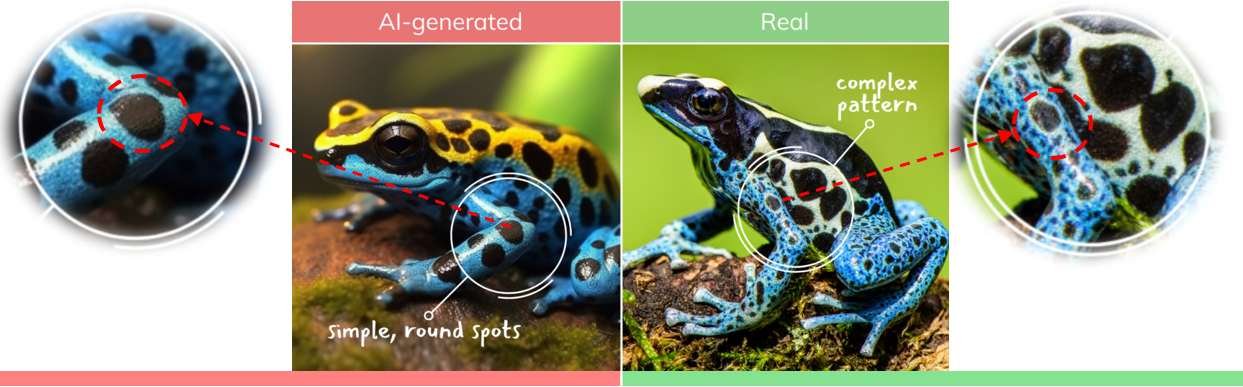
\includegraphics[width=0.9\linewidth]{ai-real-samples-1b.png}
		\begin{minipage}{0.9\linewidth}
			\caption{Ảnh tạo sinh \textit{(trái)} và ảnh thật \textit{(phải)}, được phân biệt dựa vào mức độ chi tiết trên hoa văn của đối tượng. \textit{Nguồn: \url{https://elearn.eb.com}}}
			\label{fig:ai-real-samples-1b}
		\end{minipage}
	\end{figure}\\
	%
	Bênh cạnh đó để huấn luyện mô hình \textit{"hiểu"} được các điểm bất hợp lý là bài toán khó, yêu cầu dữ liệu huấn luyện lớn và việc gán nhãn vị trí bất hợp lý trên hình ảnh cần nhiều chi phí, vì vậy hướng tiếp cận này ít được sử dụng hiện nay, tuy nhiên đây có thể là hướng phát triển tiềm năng khi kết hợp với mô hình ngôn ngữ lớn vì nó cho đưa ra được giải thích cho kết quả dự đoán.
	%
	\item Phát hiện hình ảnh giả mạo dựa vào phân tích, rút trích các đặc trưng tần số hay đặc trưng không gian trên hình ảnh. Hướng tiếp cận này mặc dù đem lại kết quả cao, ít phụ thuộc vào ngữ nghĩa của hình ảnh, tuy nhiên các kiến trúc mô hình khác nhau sẽ tạo ra những dấu vết khác nhau, do đó, thách thức lớn trong việc tìm ra đặt trưng chung và có hiệu quả trên nhiều mô hình tạo sinh (Hình~\ref{fig:gan-fingerprints-1}).
	
	\begin{figure}[h]
		\centering
		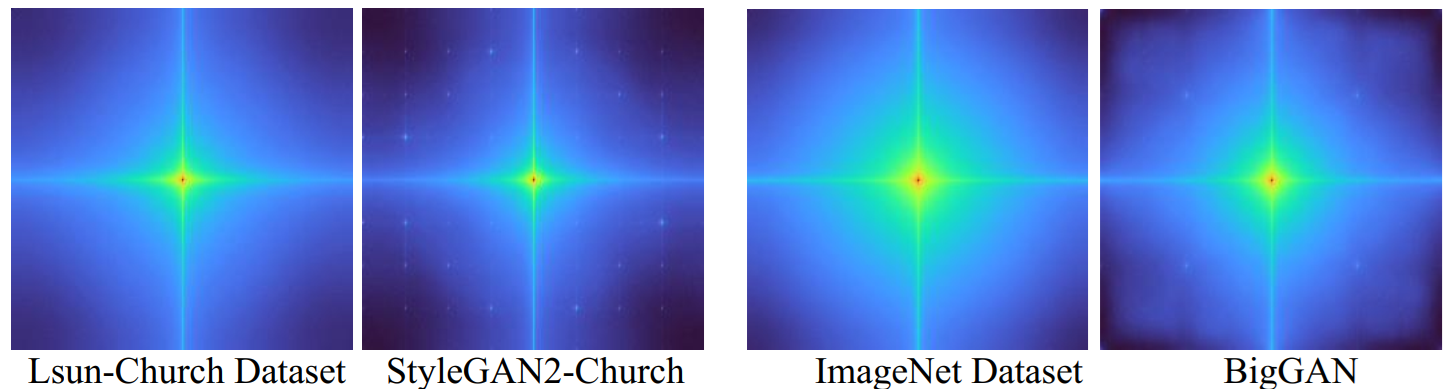
\includegraphics[width=1.0\textwidth]{gan-fingerprints-1.png}
	    \vspace{10pt} % Thay đổi khoảng cách giữa ảnh và chú thích
	    
		\begin{minipage}{\linewidth}
			\caption{Trung bình phổ Fourier của 2,000 hình ảnh từ tập dữ liệu Lsun \textit{(trái)} và ImageNet \textit{(phải)}, các dấu vết khác nhau giữa mô hình StyleGAN2 và BigGAN thể hiện ở hình 2 và 4 từ trái sang.}
			\label{fig:gan-fingerprints-1}
		\end{minipage}
	\end{figure}
	%
\end{itemize}
%
Ảnh tạo sinh rất đa dạng về nội dung, hình thức và được tạo ra theo trí tưởng tượng vô hạn của người dùng. Các hướng tiếp cận cho độ chính xác cao hiện nay, đều tận dụng sức mạnh của kỹ thuật học sâu. Tuy nhiên, dữ liệu dùng để huấn luyện các mô hình này không đủ đại diện cho toàn bộ ảnh giả mạo, cụ thể dữ liệu huấn luyện chỉ chứa một số lượng hữu hạn các đối tương trong thế giới thực, nhưng trong thực tế các đối tượng trong ảnh giả mạo có thể nằm ngoài tập huấn luyện, đây là một khó khăn cơ bản của bài toán này.

Khó khăn trong việc trả lời câu hỏi \textit{"mô hình đã dựa vào đâu để đưa ra kết luận?"}, đây là khó khăn chung của việc ứng dụng kỹ thuật học sâu, và trong nhiệm vụ phát hiện ảnh giả mạo thì yêu cầu tính \textit{"giải thích được"} càng quan trọng. Các đặc điểm thể hiện một hình ảnh là giả mạo thường không thể nhận biết một cách trực quan mà là qua sự tổng hợp rút trích đặc trưng của mạng học sâu, do tính chất phức tạp của các mô hình này, việc cung cấp giải thích rõ ràng và minh bạch cho các quyết định của mô hình là một thách thức lớn.

%
\section{Nội dung và phạm vi nghiên cứu}

\subsection{Nội dung nghiên cứu}

Đề tài tập trung vào việc phát hiện hình ảnh tạo sinh bằng cách kết hợp giữa tiền xử lý đặc thù và mô hình học sâu. Các nội dung chính bao gồm:

\begin{itemize}
	\item Khảo sát các mô hình tạo sinh hình ảnh phổ biến như GAN~\cite{Goodfellow2014GenerativeAN} và Diffusion~\cite{Ho2020DenoisingDP}.
	\item Khảo sát các phương pháp phân biệt ảnh thật và ảnh tạo sinh trong miền không gian và miền tần số.
	\item Đề xuất và thiết kế một bộ lọc không gian có chức năng tương đương với bộ lọc thông cao Fourier, nhằm làm nổi bật các đặc trưng giúp phân biệt ảnh giả.
	\item Xây dựng mô hình học sâu \gls{cnn} nhọ gọn để thực hiện phân loại ảnh thật/giả, sử dụng ảnh đầu vào đã được tiền xử lý.
	\item Huấn luyện và đánh giá mô hình trên tập dữ liệu tổng hợp từ nhiều nguồn ảnh thật và ảnh tạo sinh.
\end{itemize}

\subsection{Phạm vi nghiên cứu}

\begin{itemize}
	\item Chỉ tập trung vào ảnh tĩnh (không xử lý video hoặc ảnh động).
	%
	\item Ảnh giả mạo được tạo từ các mô hình tạo sinh phổ biến gồm GAN~\cite{Goodfellow2014GenerativeAN} và Diffusion~\cite{Ho2020DenoisingDP}.
	%
	\item Tập trung và khai thác ưu điểm của các phương pháp tiền xử lý trên miền không gian và miền tần số.
\end{itemize} 
%

\section{Đóng góp của luận văn}
Luận văn có những đóng góp cơ bản sau:
\begin{itemize}
	%
	\item Xây dựng kiến trúc mô hình đơn giản nhưng có hiệu quả cao khi kết hợp với bộ lọc mà luận văn đề xuất. Bộ phân loại sau khi huấn luyện có khả năng hoạt động tốt trên nhiều tập dữ liệu được sinh bởi nhiều loại mô hình tạo sinh khác nhau.
	%
	\item Đề xuất một bộ lọc mới làm tăng độ chính xác của mô hình, tăng tốc độ hội tụ trong quá trình huấn luyện mô hình, đồng thời phương pháp này yêu cầu số lượng phép tính nhỏ hơn nhiều phương pháp khác nhưng vẫn cho độ chính xác cao.
	%
\end{itemize}

\section{Cấu trúc của luận văn}

Luận văn được tổ chức thành 5 chương như sau:

\begin{itemize}
	\item \textbf{Chương 1 – Giới thiệu:} Trình bày bối cảnh, động lực nghiên cứu, mục tiêu, phạm vi và phát biểu bài toán. Chương cũng nêu rõ các thách thức và đóng góp chính của luận văn.
	
	\item \textbf{Chương 2 – Nghiên cứu liên quan:} Tổng quan các mô hình tạo sinh ảnh tiêu biểu và phân tích các nhóm phương pháp phát hiện hình ảnh tạo sinh, bao gồm phương pháp miền không gian, miền tần số và kết hợp.
	
	\item \textbf{Chương 3 – Phương pháp đề xuất:} Mô tả chi tiết quy trình tiền xử lý ảnh, kiến trúc mô hình học sâu, hàm mất mát sử dụng và quy trình huấn luyện mô hình.
	
	\item \textbf{Chương 4 – Thực nghiệm và đánh giá:} Trình bày các tập dữ liệu sử dụng, thiết lập thí nghiệm, các chỉ số đánh giá và kết quả so sánh với các phương pháp khác.
	
	\item \textbf{Chương 5 – Kết luận và hướng phát triển:} Tổng kết các kết quả đạt được và đề xuất một số hướng nghiên cứu mở trong tương lai.
\end{itemize}











\chapter{NGHIÊN CỨU LIÊN QUAN}
\label{Chapter2}
%
\textit{
Chương này trình bày tổng quan về các hướng nghiên cứu có liên quan đến đề tài, bao gồm hai phần chính. Phần đầu giới thiệu các mô hình tạo sinh hình ảnh tiêu biểu như GAN~\cite{Goodfellow2014GenerativeAN} và Diffusion~\cite{Ho2020DenoisingDP}, là cơ sở sinh ra các dữ liệu giả mạo ngày càng tinh vi. Phần tiếp theo tổng hợp các phương pháp phát hiện hình ảnh tạo sinh, được phân loại theo miền xử lý: miền không gian, miền tần số và phương pháp kết hợp. Việc phân tích các phương pháp hiện có giúp làm rõ thách thức kỹ thuật và định hướng xây dựng giải pháp phù hợp trong luận văn.
}\\
%
\section{Mô hình tạo sinh ảnh}
\textit{Mô hình tạo sinh ảnh là mô hình trí tuệ nhân tạo có khả năng sáng tạo ra hình ảnh mới có độ chân thật cao.}

Hiện nay, các mô hình tạo sinh ảnh chủ yếu dựa trên 3 phương pháp: Generative Adversarial Networks (GANs)~\cite{Goodfellow2014GenerativeAN}, Variational
 Autoencoders~\cite{Kingma2013AutoEncodingVB} và Diffusion Models~\cite{Ho2020DenoisingDP}. Trong đó các mô hình GANs\cite{Goodfellow2014GenerativeAN} và Diffusion~\cite{Ho2020DenoisingDP} cho chất lượng hình ảnh tốt và được sự dụng rộng rãi hiện nay. Mô hình VAEs có ưu điểm cho kết quả đầu ra đa dạng (vì mô hình học cách biểu diễn đối tượng vào 1 phân phối xác suất), do đó nó thường được kết hợp với GANs nhằm tăng khả năng linh hoạt và độ ổn định trong việc sinh dữ liệu mới.
 %
 \subsection{Mô hình GAN}
 %
 Là một kiến trúc mạng học sâu có khả năng sinh ra dữ liệu mới chủ yếu được dùng để sinh hình ảnh và âm thanh, đặc trưng của GAN~\cite{Goodfellow2014GenerativeAN} là cách huấn luyện đối kháng giữa hai nhánh mạng với mục đích cuối cùng là sinh ra dữ liệu giống với mẫu huấn luyện.\\
 \textbf{Kiến trúc của GAN~\cite{Goodfellow2014GenerativeAN}:} gồm có hai phần \gls{generator} và \gls{discriminator} (Hình ~\ref{fig:model-gan-1}).
 %
 %
 \begin{figure}[h]
 	\centering
 	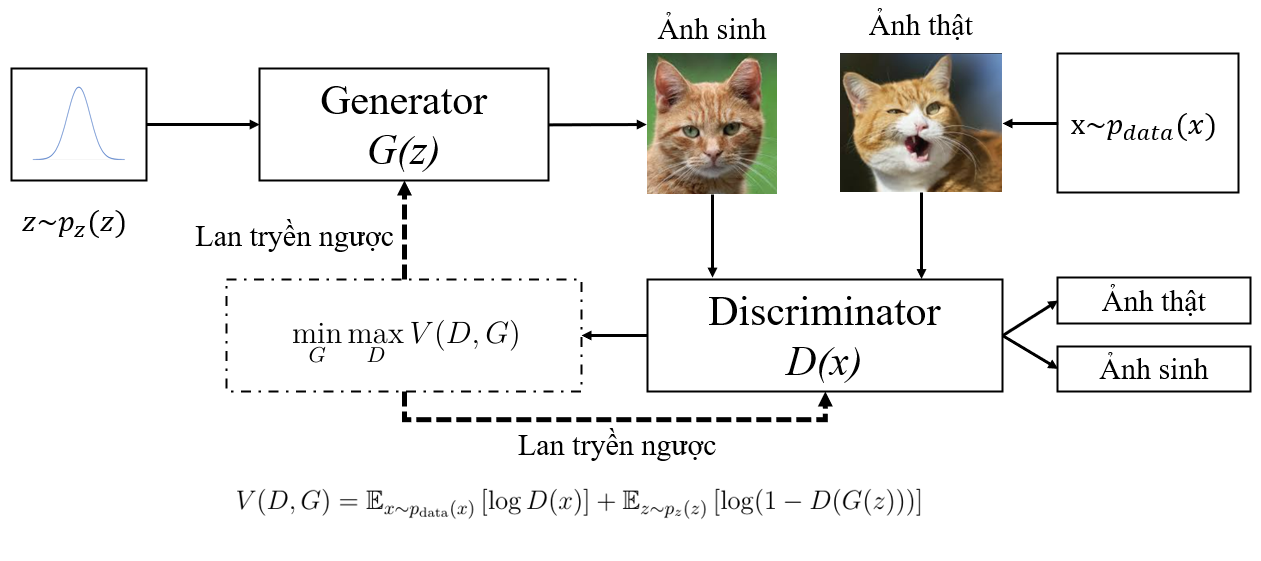
\includegraphics[width=0.9\linewidth]{Images/model-gan-1.png}
 	\caption{
 		Minh hoạ mô hình GAN.
 	}
 	\label{fig:model-gan-1}
 \end{figure}
 %
 %
 \begin{itemize}
 	 \item \Gls{discriminator}: Nhánh mạng có nhiệm vụ phân biệt một hình ảnh là thật hay được tạo ra bởi bộ \gls{generator}. Đầu vào là một hình ảnh, đầu ra là dự đoán ảnh là thật hoặc ảnh là giả.
 	 	
 	\item \Gls{generator}: Nhánh mạng này có chức năng sinh ra hình ảnh mới. Đầu vào là một nhiễu ngẫu nhiên, đầu ra là một hình ảnh được mô hình sáng tạo.	
 \end{itemize}
 %
Trong quá trình huấn luyện mạng, bộ \gls{generator} được khuyến khích tạo ra hình ảnh giống với hình ảnh thật và làm cho bộ \gls{discriminator} phân loại sai hình ảnh. Đồng thời bộ \gls{discriminator} cũng được cập nhật trọng số nhằm tăng độ chính xác trong nhiệm vụ phân loại của chính mình.

Quá trình cạnh tranh giữa hai phần này làm cho chất lượng hình ảnh được sinh bởi \gls{generator} ngày càng cao, đồng thời khả năng phân loại hình ảnh của bộ \gls{discriminator} được cải thiện liên tục.\\
%
 \textbf{Hàm mục tiêu:}
%
Mạng GAN~\cite{Goodfellow2014GenerativeAN} bao gồm hai nhánh mạng với mục tiêu huấn luyện đối ngược nhau và quá trình huấn luyện mạng diễn ra xen kẽ giữa \texttt{Generator} và \texttt{Discriminator}.\\
\[
\min_G \max_D V(D, G)
\]
Trong đó, hàm mục tiêu \( V(D, G) \) được định nghĩa là:
\[
V(D, G) = \mathbb{E}_{x \sim p_{\text{data}}(x)} \left[ \log D(x) \right] + \mathbb{E}_{z \sim p_z(z)} \left[ \log (1 - D(G(z))) \right]
\]
%
Với:
\begin{itemize}
	\item \(x\) là dữ liệu thật từ phân phối dữ liệu thật \(p_{\text{data}}(x)\).
	\item \(z\) là vectơ ngẫu nhiên từ phân phối nhiễu \(p_z(z)\), thường là phân phối Gaussian.
	\item \( \mathbb{E}_{z \sim p_z(z)} \) là kỳ vọng trên nhiễu \( z \) lấy từ phân phối \( p_z(z) \).
	\item \( G(z) \) là đầu ra của \texttt{Generator} ứng với đầu vào ngẫu nhiên $z$.
	\item \( D(G(z)) \) là xác suất mà \texttt{Discriminator} dự đoán \( G(z) \) là mẫu thật.

\end{itemize}
%
Giải thích ý nghĩa hàm mục tiêu: \gls{generator} sẽ cố gắn tối thiểu hoá $V(D,G)$ bằng cách tạo ra hình ảnh giống thật để đánh lừa \gls{discriminator} tức mong muốn $D(G(z))$ càng lớn gần \(1\) càng tốt. Ngược lại \gls{discriminator} sẽ hướng đến tôi đa hoá giá trị  $V(D,G)$  bằng cách phân loại chính xác ảnh thật và ảnh do \gls{generator} tạo ra.
%
%
\subsection{Mô hình Diffusion}
%
Là mô hình sinh ảnh chất lượng cao, được công bố trong nghiên cứu của Jonathan Ho năm 2020 với tên đầy đủ là \textit{"Mô hình xác suất khuếch tán khử nhiễu (DDPMs)~\cite{Ho2020DenoisingDP}"}, kiến trúc mô hình trong thực tế là sự kết hợp của kỹ thuật học sâu và nguyên lý của quá trình khuếch tán trong nhiệt động lực học~\cite{pmlr-v37-sohl-dickstein15}. Nguyên lý của mô hình bao gồm hai quá trình chính (Hình \ref{fig:model-diffusion-1}): quá trình khuếch tán thuận và quá trình đảo nghịch. Trong đó tạo sinh ảnh là quá trình nghịch, mô hình học cách khôi phục hình ảnh từ nhiễu.
%
\begin{figure}[h]
	\centering
	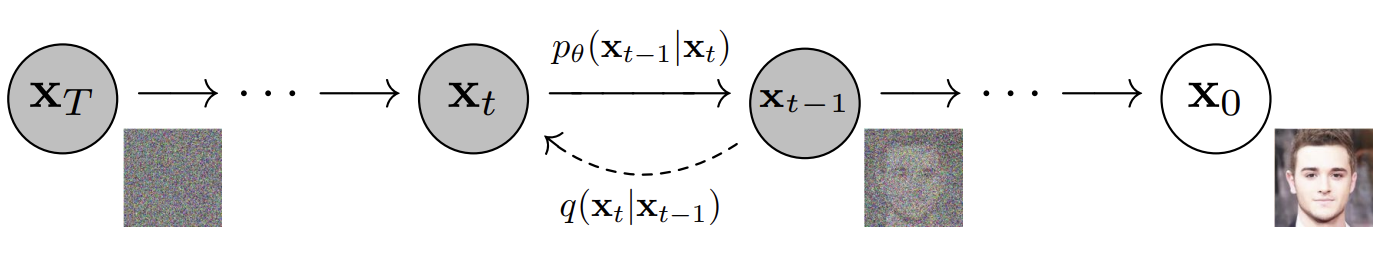
\includegraphics[width=1.0\linewidth]{Images/model-diffusion-1.png}
	\caption{
		Đồ thị có hướng mô tả hai quá trình của mô hình Diffusion. \textit{Nguồn: \cite{Ho2020DenoisingDP}}
	}
	\label{fig:model-diffusion-1}
\end{figure}\\
%
\textbf{Quá trình khuếch tán thuận:}\\
%
Trong mô hình DDPM~\cite{Ho2020DenoisingDP}, quá trình này mô phỏng lại hiện tượng khuếch tán trong tự nhiên bằng cách lặp lại nhiều lần việc thêm nhiễu Gaussian vào hình ảnh gốc cho đến khi ảnh trở thành nhiễu hoàn toàn (Hình~\ref{fig:model-forward-diffusion}).
%
Mỗi bước của quá trình được biểu diễn bằng một phân phối xác suất (Phương trình~\ref{eq:forward_diffusion}).
%
\begin{figure}[h]
	\centering
	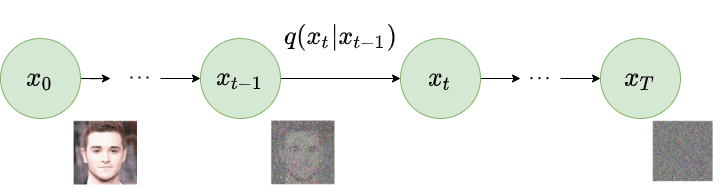
\includegraphics[width=0.8\linewidth]{Images/model-forward-diffusion.png}
	\caption{
		Quá trình khuếch tán thuận trong mô hình DDPMs. \textit{Nguồn: \cite{Ho2020DenoisingDP}}
	}
	\label{fig:model-forward-diffusion}
\end{figure}
%
\begin{equation}
	q(\mathbf{x}_t \mid \mathbf{x}_{t-1}) = \mathcal{N}(\mathbf{x}_t; \sqrt{1-\beta_t} \mathbf{x}_{t-1}, \beta_t \mathbf{I})
	\label{eq:forward_diffusion}
\end{equation}
%
Trong đó \(\mathcal{N}\) thể hiện phân phối \Gls{gaussian}, \(\beta_t \in (0,1) \) là hệ số điều chỉnh trung bình và phương sai của nhiễu được thêm vào ở bước \(t\), (trong mô hình DDPM~\cite{Ho2020DenoisingDP} thì hệ số $\beta$ là một hàm tuyến tính theo $t$), và \(\mathbf{I}\) là ma trận đơn vị, \(x_t\) là ảnh ở bước \(t\), (\(t=0\) ứng với ảnh gốc).

Toàn bộ quá trình khuếch tán thuận từ \(\mathbf{x}_0\) đến \(\mathbf{x}_T\) được mô tả bằng phương trình \ref{eq:forward_full_process}, và phương trình \ref{eq:forward_full_process2} là cách tính nhanh $q(\mathbf{x}_t \mid \mathbf{x}_0)$ trực tiếp mà không cần phải tính $\mathbf{x}_{t-1}$.

\begin{equation}
	q(\mathbf{x}_{1:T} \mid \mathbf{x}_0) = \prod_{t=1}^{T} q(\mathbf{x}_t \mid \mathbf{x}_{t-1})
	q(\mathbf{x}_t|\mathbf{x}_0)
	\label{eq:forward_full_process}
\end{equation}
%
\begin{equation}
	q(\mathbf{x}_t \mid \mathbf{x}_0) = \mathcal{N}(\mathbf{x}_t; \sqrt{\bar{\alpha}_t}\mathbf{x}_0,(1-\bar{\alpha}_t)\mathbf{I})
	\label{eq:forward_full_process2}
\end{equation} \\
%
Trong đó:
\begin{itemize}
	\item Đặt $\alpha_t := 1-\beta_t, \quad \bar\alpha_t := \prod_{s=1}^{t}\alpha_s$
\end{itemize}
%
Mục đích chính của quá trình này là tạo dữ liệu cho quá trình huấn luyện mô hình DDPM~\cite{Ho2020DenoisingDP}. Với đầu vào là \(x_t\) và đầu ra mong muốn là \({x}_0\) thuộc phân phối mong muốn (tức loại hình ảnh cần tạo sinh)\\
%
\textbf{Quá trình đảo nghịch:}\\
%
Quá trình khuếch tán thuận đã tạo ra một phân phối \Gls{gaussian} đơn giản từ hình ảnh có phân phối rất phức tạp. Quá trình đảo nghịch (Phương trình \ref{eq:reverd_process}) sẽ thực hiện khử nhiễu để thu được phân phối dữ liệu mong muốn từ một phân phối Gaussian.
%
\begin{equation}
	\mathit{p_\theta}(\mathbf{x}_{t-1} \mid \mathbf{x}_t) = \mathcal{N}(\mathbf{x}_{t-1}; \frac{1}{\sqrt{\alpha_t}}(\mathbf{x}_t - \frac{1-\alpha_t}{\sqrt{1-\bar\alpha_t}}\mathbf{\epsilon}_t, \frac{1-\bar\alpha_{t-1} }{1-\bar\alpha_t}.\beta_t)
	\label{eq:reverd_process}
\end{equation}
%

Trong thực tế, người ta dùng một mạng nơ-ron để dự đoán nhiễu đã được thêm vào của từng bước thời gian chứ không trực tiếp hình ảnh ở bước thời gian trước đó.\\
%
\textbf{Thuật toán huấn luyện mô hình:}\\
%
Quá trình được mô tả chi tiết trong hình ~\ref{fig:model-diffusion-training-1}, và được diễn giải như sau:
\begin{itemize}
	\item Tập ảnh huấn luyện $\mathbf{x}$ được chia thành các mẻ (\textit{batch}) $\mathcal{B}$.
	%
	\item Ứng với mỗi lần duyệt qua hình ảnh $\mathbf{x}_i$ trong $\mathcal{B}$, chọn tuỳ ý một bước thời gian $\mathit{t}\sim Uniform[1,...T]$, và một nhiễu $\mathbf{\epsilon} \in \mathcal{N}(0,I)$.
	%
	\item Thêm nhiễu ở bước thời gian $\mathit{t}$ vào hình ảnh $\mathbf{x}_i$ ban đầu để thu được ảnh nhiễu của bước $\mathit{t}$. Lượng nhiễu được thêm sẽ phụ thuộc vào $\mathit{t}$ và $\mathbf{\epsilon}$.
	%
	\item Cho hình ảnh $\mathbf{x}_i$ đã thêm nhiễu vào mô hình ($\mathbf{g}_t(.)$) để dự đoán nhiễu được thêm vào ở bước trước.
	%
	\item Tính giá trị hàm mục tiêu $\ell_i$ là bình phương sai số giữa nhiễu dự đoán và nhiễu thực sự $\epsilon$
	\item Cập nhật trọng số cho mô hình và lặp lại quá trình.
\end{itemize}
%
\begin{figure}[h]
	\centering
	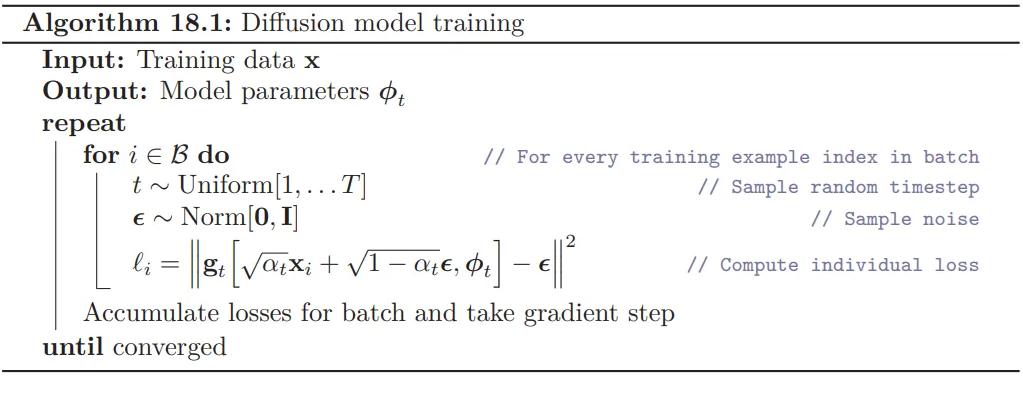
\includegraphics[width=0.9\linewidth]{Images/model-diffusion-training-1.png}
	\caption{
		Mô tả thuật toán huấn luyện mô hình Diffusion.
	\textit{Nguồn: \cite{prince2023understanding}}
	}
	\label{fig:model-diffusion-training-1}
\end{figure}
%
\textbf{Thuật toán sinh ảnh của mô hình Diffusion:}\\
%
Sau khi đã huấn luyện xong mô hình Diffusion~\cite{Ho2020DenoisingDP}, quá trình sinh ra ảnh mới từ một điểm dữ liệu trong phân phối chuẩn diễn ra như sau.
%
\begin{itemize}
	\item Tạo một nhiễu ngẫu nhiên $\mathbf{z}_T \in \mathcal{N}(0,I)$, với $\mathit{T}$ là bước thời gian được chọn tuỳ ý ($\mathit{T}$ càng lớn thì chất lượng ảnh sẽ cao nhưng đồng thời cũng tăng thời gian tạo ảnh).
	\item Ứng với mỗi bước thời gian $\mathit{t} \in [T,T-1,...,2]$ ta thực hiện quá trình khử nhiễu dần dần đến khi thu được ảnh không nhiễu.
		\begin{itemize}
			\item Dự đoán nhiễu ở bước $\mathit{t-1}$, khử nhiễu ta thu được ảnh $\mathbf{\hat{z}}_{t-1}$.
			\item Thêm vào $\mathbf{\hat{z}}_{t-1}$ một lượng nhiễu $\mathbf{\epsilon} \in \mathcal{N}_\epsilon(0,I)$ (nhằm mô phỏng lại quá trình thuận)
			\item Lặp lại quá trình cho đến khi thu được $\mathbf{z}_0$ (ở đây $\mathbf{x=z_0}$ là ảnh tạo sinh cuối cùng)
		\end{itemize}

\end{itemize}
%
\begin{figure}[h]
	\centering
	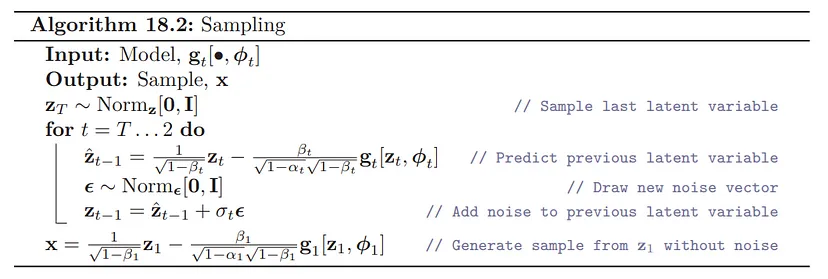
\includegraphics[width=0.9\linewidth]{Images/model-diffusion-sampling-1.png}
	\caption{
		Mô tả quá trình sinh ảnh mô hình Diffusion.
		\textit{Nguồn: \cite{prince2023understanding}}
	}
	\label{fig:model-diffusion-sampling-1}
\end{figure}
%
\section{Phát hiện hình ảnh tạo sinh}
%
Luận văn tập trung ta nghiên cứu và tiếp cận nhóm phương pháp phát hiện hình ảnh tạo sinh dựa trên phân tích, rút trích đặc trưng trên \textit{miền không gian} và \textit{miền tần số} của hình ảnh.
%
%
\subsection{Nhóm phương pháp tiếp cận trên miền không gian}
Nhóm phương pháp này dựa vào phân tích, rút trích các đặc trưng từ tín hiệu màu sắc, biên cạnh, hoặc nhiễu trực tiếp từ điểm ảnh.\\
\textbf{Phương pháp của Scott McCloskey (2018)}~\cite{8803661} đã phân tích cấu trúc của mạng GANs~\cite{Goodfellow2014GenerativeAN} và tập trung đến cách mà mô hình tạo ra màu sắc. Trong quá trình sinh ảnh, các giá trị màu đã được mô hình chuẩn hoá nhằm hạn chế số lượng các điểm ảnh bão hoà\footnotemark\footnotetext{là giá trị cường độ của một hoặc nhiều kênh màu đạt được cực đại (255) và cực tiểu (0) đối với định dạng 8-bit cho mỗi kênh màu}.
%
\begin{figure}[h]
	\centering
	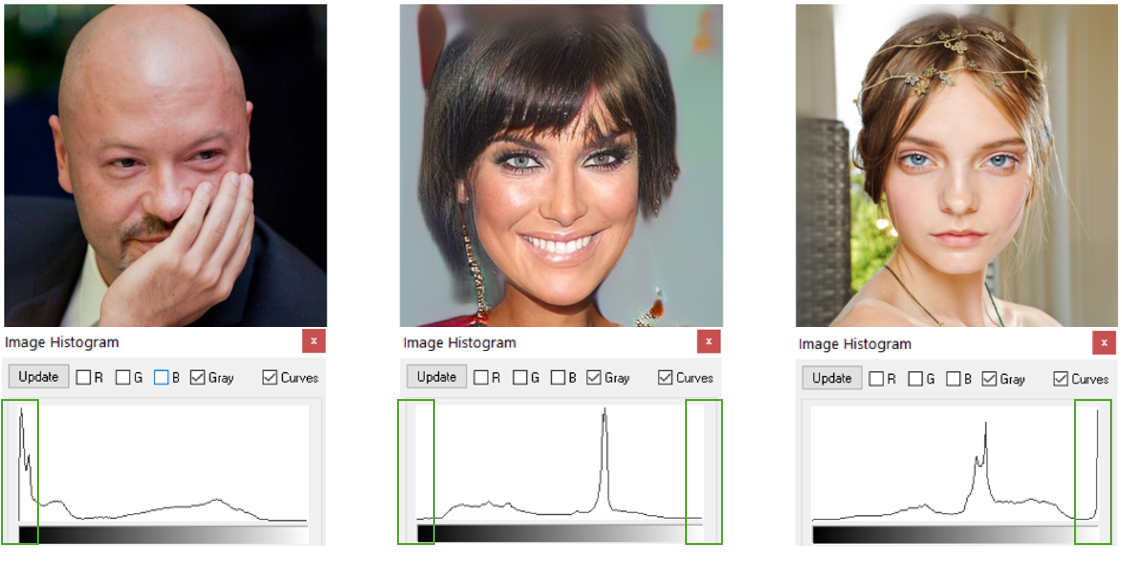
\includegraphics[width=0.9\linewidth]{Images/histograms-gan-real-1.png}
	\caption{
		Một ví dụ về sự thiếu vắng vùng bảo hoà (vùng đánh dấu màu xanh lá nằm ở 2 bên biểu đồ \gls{histogram} của ảnh tạo sinh (\textit{giữa}), trong khi ảnh thật (\textit{trái}) và (\textit{phải}) có sự xuất hiện của vùng bảo hoà. \textit{Nguồn: \cite{8803661}}
		}
	\label{fig:histograms-gan-real-1}
\end{figure}
%
Hơn nữa, những lớp mạng cuối cùng có nhiệm vụ tổng hợp ba kênh màu cơ bản đỏ, xanh lá cây và xanh lam từ một ma trận nhiều chiều bằng cách sử dụng các lớp tích chập (cùng một bộ trọng số cho tất cả điểm ảnh), tuy nhiên tỉ lệ trọng số giữa các kênh có cấu trúc khác xa so với bộ lọc 3 màu cơ bản trong máy ảnh (Hình~\ref{fig:colors-weight-gan-camera-1b}), qua quan sát tác giả nhận thấy rằng các thành phần màu sắc có xu hướng tương quan mạnh với nhau trong mạng GANs~\cite{Goodfellow2014GenerativeAN}, ngược lại đối với hình ảnh thật, phổ của bộ lọc màu có sự chồng chéo và đỉnh của chúng không trùng nhau (các vị trí đỉnh nơi mũi tên màu đỏ hướng đến trong hình~\ref{fig:colors-weight-gan-camera-1b}) . Hai quan sát trên là cơ sở mà Scott McCloskey dùng để phân biệt hình ảnh tạo sinh.
%
Triển khai phương pháp của mình trong thực tế Scott McCloskey và cộng sự đã tinh chỉnh mạng FMIHNet~\cite{Chen2018FocusMD} được đề xuất bởi Cheng (2018)\footnote{FMIHNet là kiến trúc mạng cho phép phân biệt được các dấu vết làm mờ giả tạo trên ảnh được chỉnh sửa và lấy nét quan học có trên ảnh thật có đầu vào là biểu đồ tần suất (\gls{histogram}) của hình ảnh.}
%
\begin{figure}[h]
	\centering
	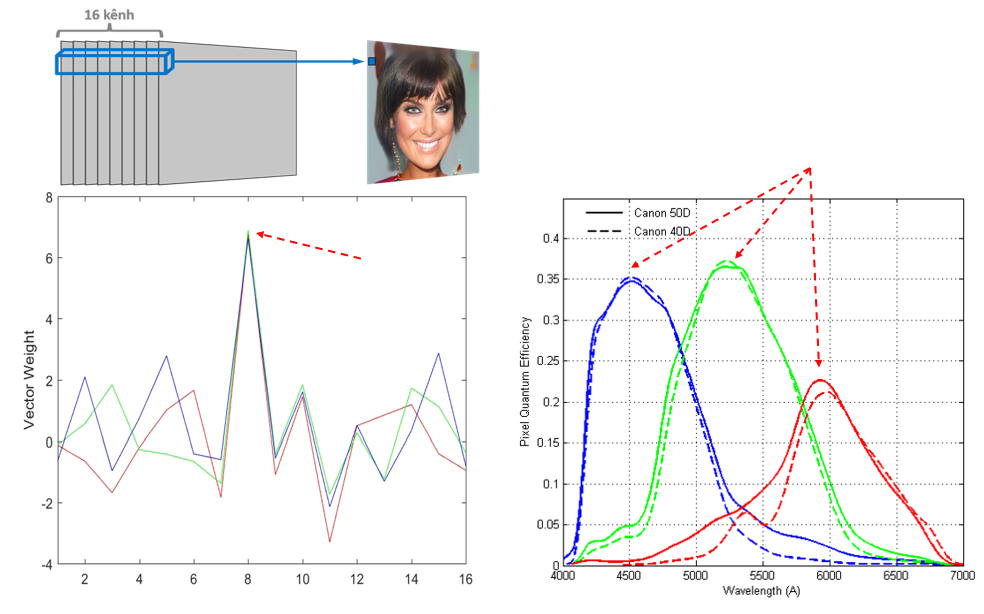
\includegraphics[width=0.9\linewidth]{Images/colors-weight-gan-camera-1b.png}
	\begin{minipage}{0.9\linewidth}
		\caption{Cấu trúc trọng số của lớp tích chập cuối trong mạng GANs  \textit{(trái)} và Phổ bộ lọc màu của 2 máy ảnh Canon 50D và Canon 40D \textit{(phải)}. \textit{Nguồn: \cite{8803661}}}
		\label{fig:colors-weight-gan-camera-1b}
	\end{minipage}
\end{figure}\\
%
-\textbf{Ưu điểm của phương pháp:} Đơn giản, hiệu quả, dữ liệu phân tích rõ ràng và quan sát được một cách trực quan.\\
-\textbf{Hạn chế của phương pháp:} Các dấu vết về sự thiếu vắng các điểm ảnh bảo hoà trong ảnh tạo sinh dễ dàng bị loại bỏ có chủ đích để qua mặt phương pháp này.\\
%
\textbf{Phương pháp Gram-Net~\cite{9157447}} do Liu và cộng sự đề xuất năm 2020. Phương pháp này phân biệt ảnh thật và ảnh giả mạo dựa vào các \gls{texture} của ảnh.\\
%
Tác giả đã thực hiện thử nghiệm để kiểm tra mức độ ảnh hưởng của kết cấu bề mặt ảnh tác động lên hiệu suất của mô hình phân loại. Thực hiện cắt khu vực chứa vùng da mặt trên ảnh và áp dụng lần lược kỹ thuật tiền xử lý (Hình~\ref{fig:gray-scale-and-texture-1}), trước khi đưa hình ảnh vào huấn luyện bộ phân loại sử dụng kiến trúc CNN~\cite{Krizhevsky2012ImageNetCW}.
%
%
\begin{figure}[h]
	\centering
	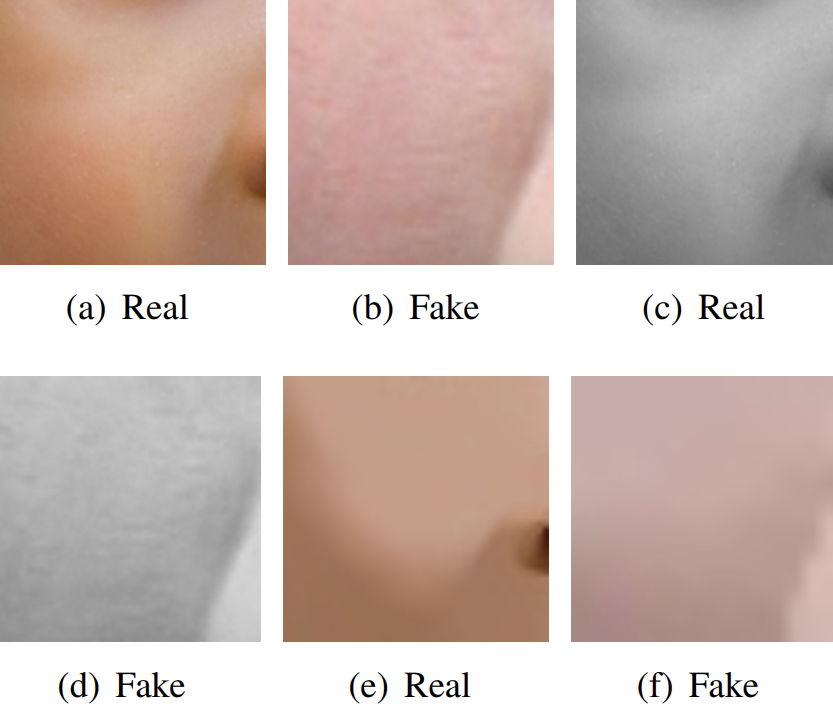
\includegraphics[width=0.8\linewidth]{Images/gray-scale-and-texture-1.png}
	\begin{minipage}{0.9\linewidth}
		\caption{Ảnh gốc (a-b), ảnh biến đổi Gray-scale (c-d), ảnh áp dụng bộ lọc \textit{L0} (e-f)). \textit{Nguồn: \cite{9157447}}}
		\label{fig:gray-scale-and-texture-1}
	\end{minipage}
\end{figure}
%
%
\begin{itemize}
	\item \textit{Chuyển các mẫu về ảnh xám (Gray-scale):} Nhằm loại bỏ ảnh hưởng của màu sắc.
	\item \textit{Áp dụng bộ lọc L0~\cite{10.1145/2070781.2024208}:} Bộ lọc làm mịn các kết cấu nhỏ, tuy nhiên vẫn giữ lại màu sắc và hình dạng của đối tượng.
\end{itemize}
%
%
Kết quả thử nghiệm chỉ ra rằng (Bảng~\ref{tab:human_vs_cnns_1} dòng 4-5): Mô hình phân loại được huấn luyện với các hình ảnh \gls{grayscale} nhưng vẫn chứa đầy đủ \gls{texture} cho độ chính xác giảm nhẹ so với mô hình huấn luyện trên ảnh gốc. Điều này chứng tỏ màu sắc không ảnh hưởng nhiều đến mô hình phân loại.

Ngược lại, hiệu suất của mô hình giảm mạnh (khoảng 20\%) khi áp dụng bộ lọc \textit{L0}. Cho thấy \gls{texture} đóng vai trò quan trọng trong việc phân biệt ảnh tạo sinh, và mô hình \gls{cnn} cũng đã trích xuất được các đặc trưng này sau quá trình huấn luyện.
% Nội dung của table1.tex
\begin{center}
\begin{table}[htbp]
	\centering
	\begin{tabular}{p{3cm}|p{3cm}|p{2.5cm}|p{2cm}|p{2cm}}
		\hline
		\multirow{2}{*}{Input} & \multirow{2}{*}{Human vs. CNNs} & {StyleGAN vs. CelebA-HQ} & {StyleGAN vs. FFHQ} & {PGGAN vs. CelebA-HQ} \\ 
		\hline
		{Full image} & {Human Beings} & 75.15\% & 63.90\% & 79.13\% \\ 
		{Full image} & {ResNet} & 99.99\% & 99.96\% & 99.99\% \\ 
		\hdashline
		{Original (skin)} & {ResNet} & 99.93\% & 99.61\% & 99.96\% \\ 
		{Gray-scale (skin)} & {ResNet} & 99.76\% & 99.47\% & 99.94\% \\ 
		{L0-filtered (skin)} & {ResNet} & 78.64\% & 76.84\% & 72.02\% \\ 
		\hline
	\end{tabular}
	\caption{Bảng so sánh kết quả huấn luyện bộ phân loại ứng với từng kĩ thuật tiền xử lý (\textit{dòng 3-5}), và hiệu suất của của con người (\textit{dòng 1}) so với mạng học sâu. \textit{Nguồn:\cite{9157447}}}
	\label{tab:human_vs_cnns_1}
\end{table}
\end{center}
%
%
-\textbf{Đóng góp của phương pháp:}
Phân tích và thực hiện thử nghiệm chứng tỏ tầm quan trọng của \gls{texture} trong bài toán phát hiện ảnh tạo sinh.
%
Đề xuất kiến trúc khối Gram, cho phép tích hợp các \gls{backbone} CNN~\cite{Krizhevsky2012ImageNetCW} tạo nên kiến trúc Gram-Net~\cite{9157447}, tăng cường độ chính xác so với mạng các mạng \gls{cnn} cơ bản như ResNet~\cite{He2015DeepRL}.\\
%
-\textbf{Hạn chế của phương pháp}:
Yêu cầu độ phức tạp của mô hình lớn, đồng thời hiệu suất giảm mạnh khi thực hiện kiểm tra chéo trên các tập dữ liệu khác nhau.\\
%
\textbf{Phương pháp Fusing}~\cite{9897820} công bố trong bài báo \textit{Fusing Global and Local Features for Generalized AI-Synthesized Image Detection} của Yan-Ju năm 2022.\\
Trong nghiên cứu này Yan-Ju và cộng sự thiết kế mô hình (Hình \ref{fig:model-fusing-architecture-1}) gồm hai nhánh, nhằm kết hợp đặc trưng không gian toàn cục từ toàn bộ hình ảnh và các đặc trưng cục bộ từ nhiều \gls{patch}.
%
\begin{figure}[h]
	\centering
	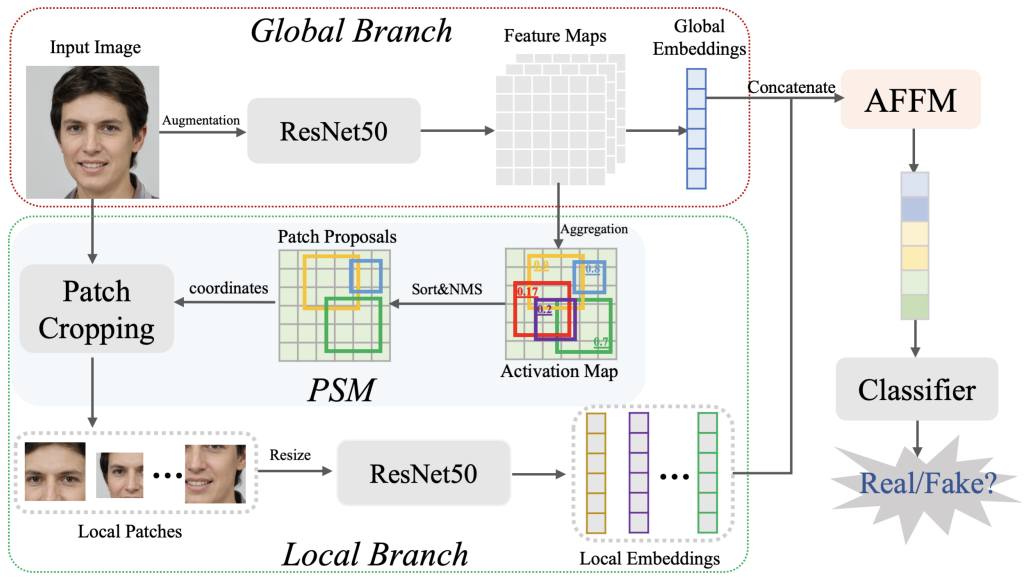
\includegraphics[width=1.0\linewidth]{Images/model-fusing-architecture-1.png}
	\begin{minipage}{0.9\linewidth}
		\caption{Kiến trúc mô hình Fusing \textit{Nguồn: \cite{9897820}}}
		\label{fig:model-fusing-architecture-1}
	\end{minipage}
\end{figure}
%

-Nhánh mô hình \textit{Global Branch:} 
%
Dùng \gls{backbone} ResNet50~\cite{He2015DeepRL} để trích xuất đặc trưng toàn cục. Cụ thể đầu vào là hình ảnh màu $\mathbb{I} \in \mathbb{R}^{3 \times w \times h}$, bản đồ đặc trưng toàn cục $\mathbb{F} \in \mathbb{R}^{C \times W_f \times H_f}$ thu được từ lớp tích chập cuối cùng của ResNet50~\cite{He2015DeepRL}.

-Nhánh mô hình \textit{Local Branch:} Có nhiệm vụ trích xuất thông tin từ một số mảnh vá mang nhiều thông tin nhất.

\begin{itemize}
	\item Cơ chế Attention~\cite{Vaswani2017AttentionIA} được áp dụng để tính toán lượng thông tin của mảnh vá, và được tích hợp bên trong mô-đun \textit{Patch Selection Module (PSM)}, với đầu vào là bản đồ đặc trưng toàn cục $\mathbb{F}$ và đầu ra là toạ độ của các \gls{patch} trên ảnh $\mathbb{I}$ đủ tiêu chuẩn.
	%
	\item Vec-tơ đặc trưng cục bộ được tính tương tự với đặc trưng toàn cục (tức sử dụng \gls{backbone} ResNet50~\cite{He2015DeepRL}), tuy nhiên đầu vào là những \gls{patch} (được chọn ra bởi mô-đun PSM), thay vì là toàn bộ hình ảnh.
	%
	\item Đặc trưng toàn cục và đặc trưng cục bộ được kết hợp với nhau thông qua cơ chế \gls{attention}~\cite{Vaswani2017AttentionIA} có trong mô-đun \textit{Attention-based Feature Fusion}, trước khi đưa qua bộ phân loại.
\end{itemize}
%
-\textbf{Ưu điểm của phương pháp:}
%
Cho phép kết hợp đặc trưng toàn cục và đặc trưng cục bộ của hình ảnh, giúp tăng tính khái quá của mô hình.\\
%
-\textbf{Hạn chế của phương pháp:}
Kiến trúc có 2 nhánh mạng và đều sử dụng \gls{backbone} ResNet50~\cite{He2015DeepRL}, nghĩa là độ phức tạp của mô hình tăng gấp 2 lần.\\
%
\textbf{Một số phương pháp cùng hướng tiếp cận:}
%

Công trình nghiên cứu \textit{Multi-Attentional Deepfake Detection} của Zhao và cộng sự (2021)~\cite{Zhao_2021_CVPR} đã trích xuất và tổng hợp các \gls{texture} ở nhiều mức độ phóng to khác nhau, kết hợp với mô-đun Attention~\cite{Vaswani2017AttentionIA} nhằm tích hợp chúng với các đặc trưng ngữ nghĩa trừu tượng hơn từ các lớp sâu của mạng.

Nan-Zhong công bố nghiên cứu \textit{Rich and Poor Texture Contrast: A Simple yet Effective Approach for AI-generated Image Detection}~\cite{zhong2023rich}(2023). Phương pháp này khai thác sự tương phản trong mối tương quan giữa các \gls{richtexteregion} và các \gls{poortexteregion}, bằng phẳng trong một bức ảnh. \\
%
Trước tiên, cắt hình ảnh gốc thành nhiều \gls{patch} và tái cấu trúc chúng thành ảnh chứa \gls{richtexteregion} và ảnh chứa \gls{poortexteregion}. Sau đó sử dụng mạng \gls{cnn}~\cite{Krizhevsky2012ImageNetCW} rút trích, kết hợp các loại đặc trưng khác nhau. Các đặc trưng sau khi tổng hợp sẽ được đưa qua một mạng nơ-ron đa tầng đơn giản làm nhiệm vụ phân loại ảnh thật/giả mạo (Hình \ref{fig:model-rich-poor-textture-1}).
%
\begin{figure}[h]
	\centering
	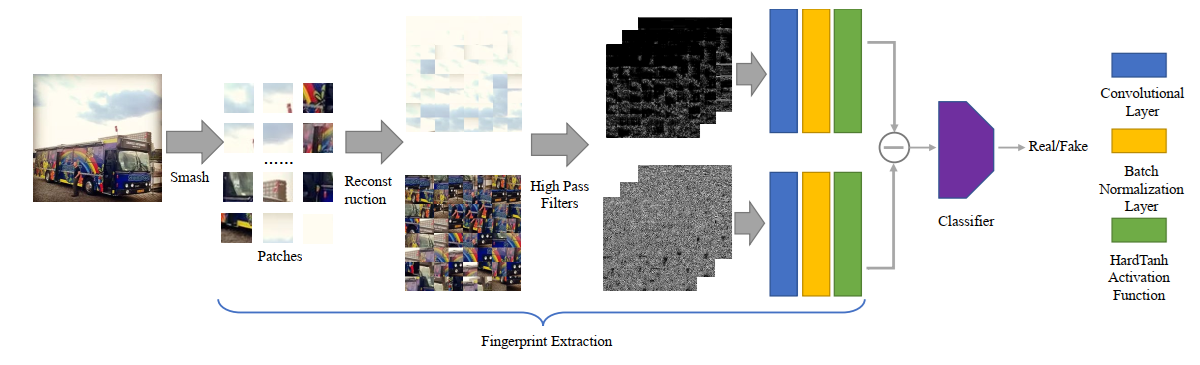
\includegraphics[width=1.0\linewidth]{Images/model-rich-poor-textture-1.png}
	\begin{minipage}{0.9\linewidth}
		\caption{Mô tả phương pháp Rich Poor Texture Contrast của Nang-Zhong \textit{Nguồn: \cite{zhong2023rich}}}
		\label{fig:model-rich-poor-textture-1}
	\end{minipage}
\end{figure}\\
%
-\textbf{Ưu điểm của phương pháp:}
Việc tái cấu trúc lại hình ảnh thành \gls{richtexteregion} và \gls{poortexteregion} giúp mô hình trích xuất đặc trưng có hiệu quả hơn, làm tăng độ chính xác của mô hình. Hơn nữa việc tại cấu trúc này sẽ phá vỡ ngữ nghĩa của hình ảnh, làm giảm hiện tượng thiên lệch mẫu huấn luyện, giúp mô hình nâng cao mức độ khái quát.\\
-\textbf{Hạn chế của phương pháp:}
Khó khăn khi lựa chọn kích thước \gls{patch} phù hợp, vì mỗi hình ảnh sẽ có cấu trúc khác nhau. Thực nhiệm cũng cho thấy việc sử dụng kích thước \gls{patch} khác với quá trình huấn luyện, sẽ làm giảm độ chính xác của phương pháp.
%
\subsection{Nhóm phương pháp tiếp cận miền tần số}
Nhóm phương pháp này thực hiện chuyển đổi hình ảnh từ miền không gian sang miền tần số bằng các phép biến đổi như \gls{fft}~\cite{Arunachalam2013TheFF} hoặc \gls{dft}~\cite{1672377}.
Khi tập trung vào các đặc điểm tần số, các phương pháp này cho kết quả phát hiện các dấu vết giả tạo tốt hơn so với miền không gian.\\
%
\textbf{Unmasking DeepFakes with simple Features}~\cite{durall2019unmasking} (2019) của Durall.
Bước đầu hình ảnh được chuyển thành phổ công suất bằng \gls{dft}, sau đó áp dụng phương pháp \gls{azimuthalaveraging} để chuyển phổ công suất từ hai chiều về một chiều nhằm mục đích phù hợp cho quá trình huấn luyện bộ phân loại (Hình ~\ref{fig:model-unmasking-deepfakes-1}).
%
\begin{figure}[h]
	\centering
	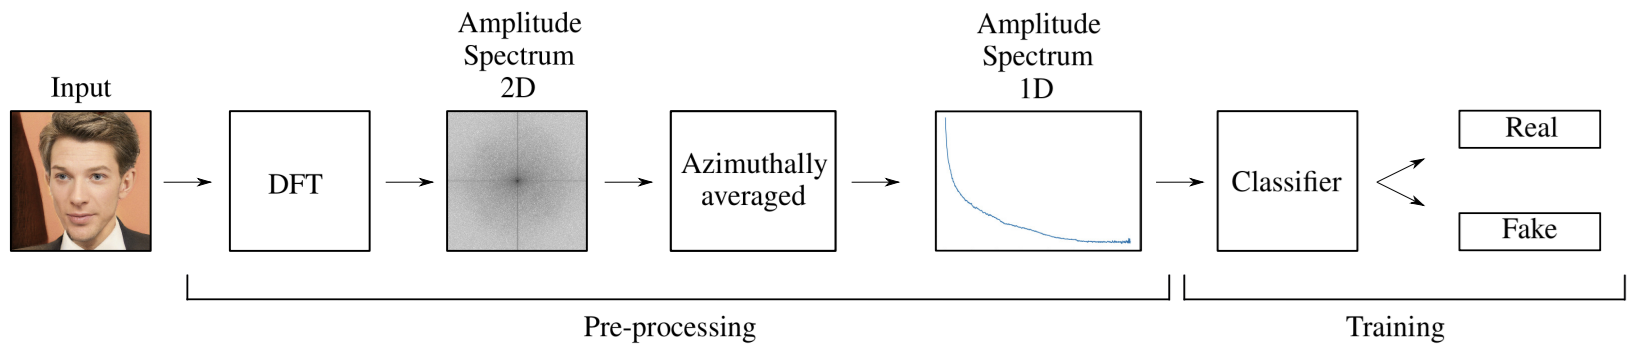
\includegraphics[width=1.0\linewidth]{Images/model-unmasking-deepfakes-1.png}
	\begin{minipage}{0.9\linewidth}
		\caption{Tổng quan về quy trình xử lý trong phương pháp của Durall. \textit{Nguồn: \cite{durall2019unmasking}}}
		\label{fig:model-unmasking-deepfakes-1}
	\end{minipage}
\end{figure}\\
%
%
-\textbf{Nhận xét phương pháp:}
Đây là phương pháp đơn giản, yêu cầu dữ liệu huấn luyện ít, và sử dụng các bộ phân loại cơ bản như: \gls{svm}, \gls{kmeans}, \gls{logisticregression} nhưng cho kết quả tương đối cao trên một số bộ dữ liệu cụ thể được dùng trong bài báo. Các kết quả thử nghiệm cho thấy tiềm năng hứa hẹn của việc sử dụng các phương pháp tiếp cận trên miền tần số trong việc phát hiện ảnh tạo sinh.\\
%
\textbf{Các phân tích của Frank}\cite{Frank2020LeveragingFA} cung cấp trong bài báo \textit{"Leveraging Frequency Analysis for Deep Fake Image Recognition (2020)"} chỉ ra bằng chứng biểu diễn tần số của hình ảnh sẽ làm lộ ra các dấu vết tạo tác mà mô hình để lại, quan sát biểu đồ phổ (Hình \ref{fig:dct-spectra-1}) được vẽ từ ảnh trung bình của 10,000 hình ảnh được thực hiện \gls{dct} trong tập dữ liệu \textit{Stanford dog} có thể nhận thấy được bằng mắt thường một số khác biệt giữa phổ của ảnh thật (vị trí ngoài cùng bên trái) so với các ảnh còn lại.
%
\begin{figure}[h]
	\centering
	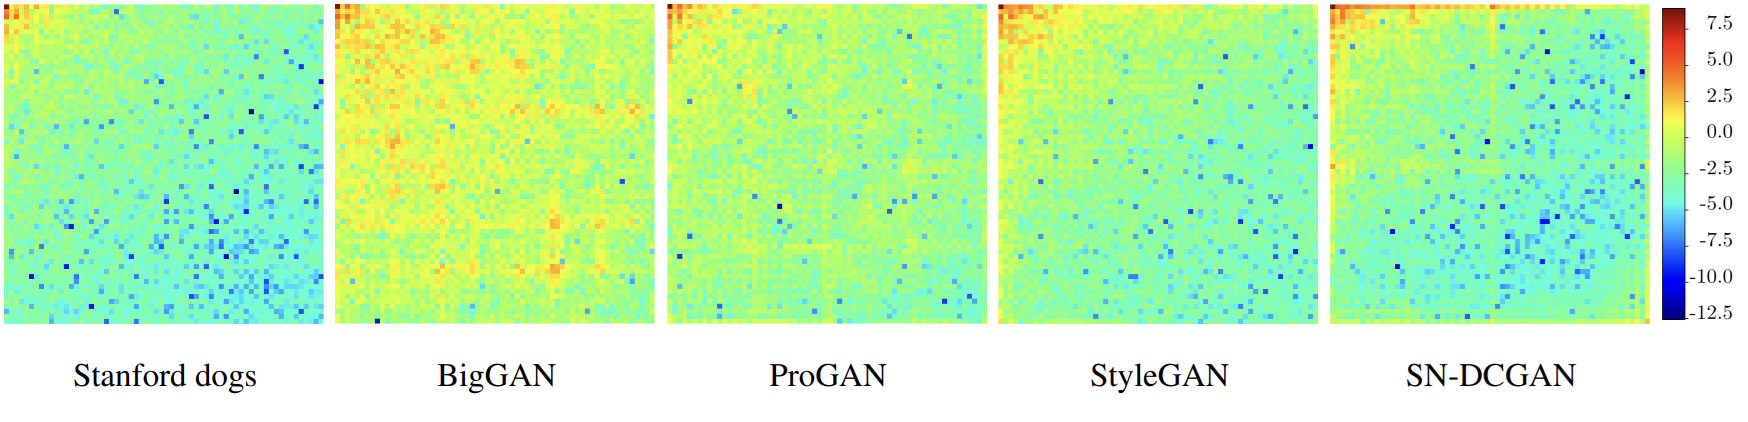
\includegraphics[width=1.0\linewidth]{Images/Stanford-dog-data-set-DCT-spectra.png}
	\begin{minipage}{0.9\linewidth}
		\caption{Phổ hình ảnh được tạo ra bởi các mạng nơ-ron khác nhau được đào tạo trên tập dữ liệu \textit{Stanford dog.} \textit{Nguồn: \cite{Frank2020LeveragingFA}}}
		\label{fig:dct-spectra-1}
	\end{minipage}
\end{figure}
%
Cụ thể, với ảnh thật, năng lượng tập trung ở khu vực tần số thấp (góc trên bên trái) và dần đều về phía tần số cao (góc dưới bên phải), trong khi đó ở ảnh giả mạo, sẽ xuất hiện đột ngột các dãy tần số có năng lượng cao, theo quy luật (các đường tương tự như lưới vuông trong hình). Tiếp tục mở rộng các thử nghiệm của mình Frank khảo sát ảnh hưởng của toán tử \gls{up-sampling} tác động lên hình ảnh tạo sinh, bằng cách vẽ lại biểu đồ phổ trung bình (xem Hình~\ref{fig:frank-spectrum-up-sampling-1}) sau khi thay thế các toán tử \gls{up-sampling} khác nhau gồm: \gls{nearestneighbor}, \gls{bilinear}, \gls{binomialupsampling}. Tác giả huấn luyện 3 phiên bảng StyleGAN~\cite{karras2019style} trên tập dữ liệu LSUN-Bedroom~\cite{Yu2015LSUNCO}, phiên bản đầu tiên giữ nguyên toán tử \gls{bilinear}, phiên bản thứ hai và ba lần lượt thay thế bằng \gls{nearestneighbor} và \gls{binomialupsampling}.
Sự khác biệt của các dấu vết tạo tác xuất hiện rõ ràng dưới dạng lưới ô vuông trong hình \ref{fig:frank-spectrum-up-sampling-1} ứng với \gls{nearestneighbor},\gls{bilinear} và rất mờ với \gls{binomialupsampling} khi so sánh với ảnh thật (ngoài cùng bên trái).
%
\begin{figure}[h]
	\centering
	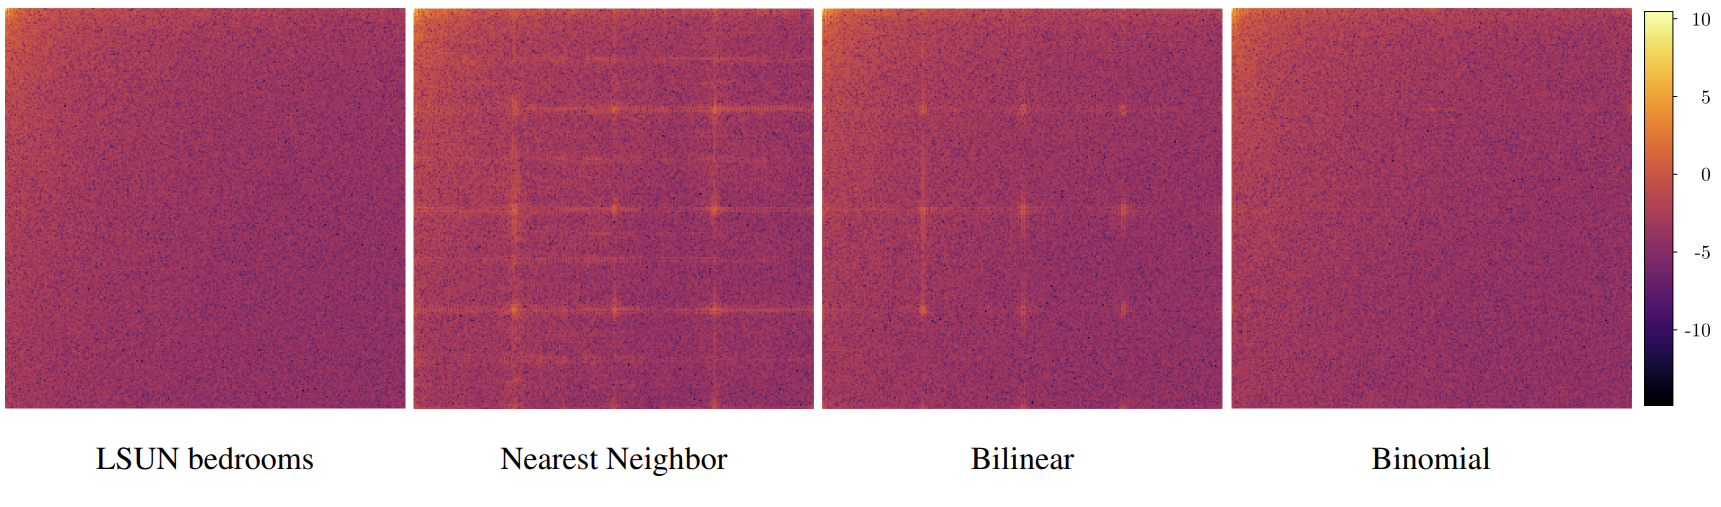
\includegraphics[width=1.0\linewidth]{Images/frank-spectrum-up-sampling-1.png}
	\begin{minipage}{0.9\linewidth}
		\caption{Phổ hình ảnh tương ứng với các kỹ thuật \gls{up-sampling} khác nhau.\textit{Nguồn: \cite{Frank2020LeveragingFA}}}
		\label{fig:frank-spectrum-up-sampling-1}
	\end{minipage}
\end{figure}
%

Ngoài ra, bằng thực nghiệm, tác giả chứng minh rằng bộ phân loại dựa trên biểu diễn tần số mang lại độ chính xác cao, đồng thời yêu cầu ít tham số hơn so với giữ nguyên giá trị điểm ảnh. Hình~\ref{fig:frank-acc-comparison-1} cung cấp thông tin quá trình huấn luyện bộ phân loại sử dụng kiến trúc \gls{cnn}, kết quả cho thấy tốc độ hội tụ nhanh vượt trội của mô hình khi áp dụng \gls{dct}~\cite{1672377} cho hình ảnh so với giữ nguyên giá trị điểm ảnh gốc.
%
\begin{figure}[h]
	\centering
	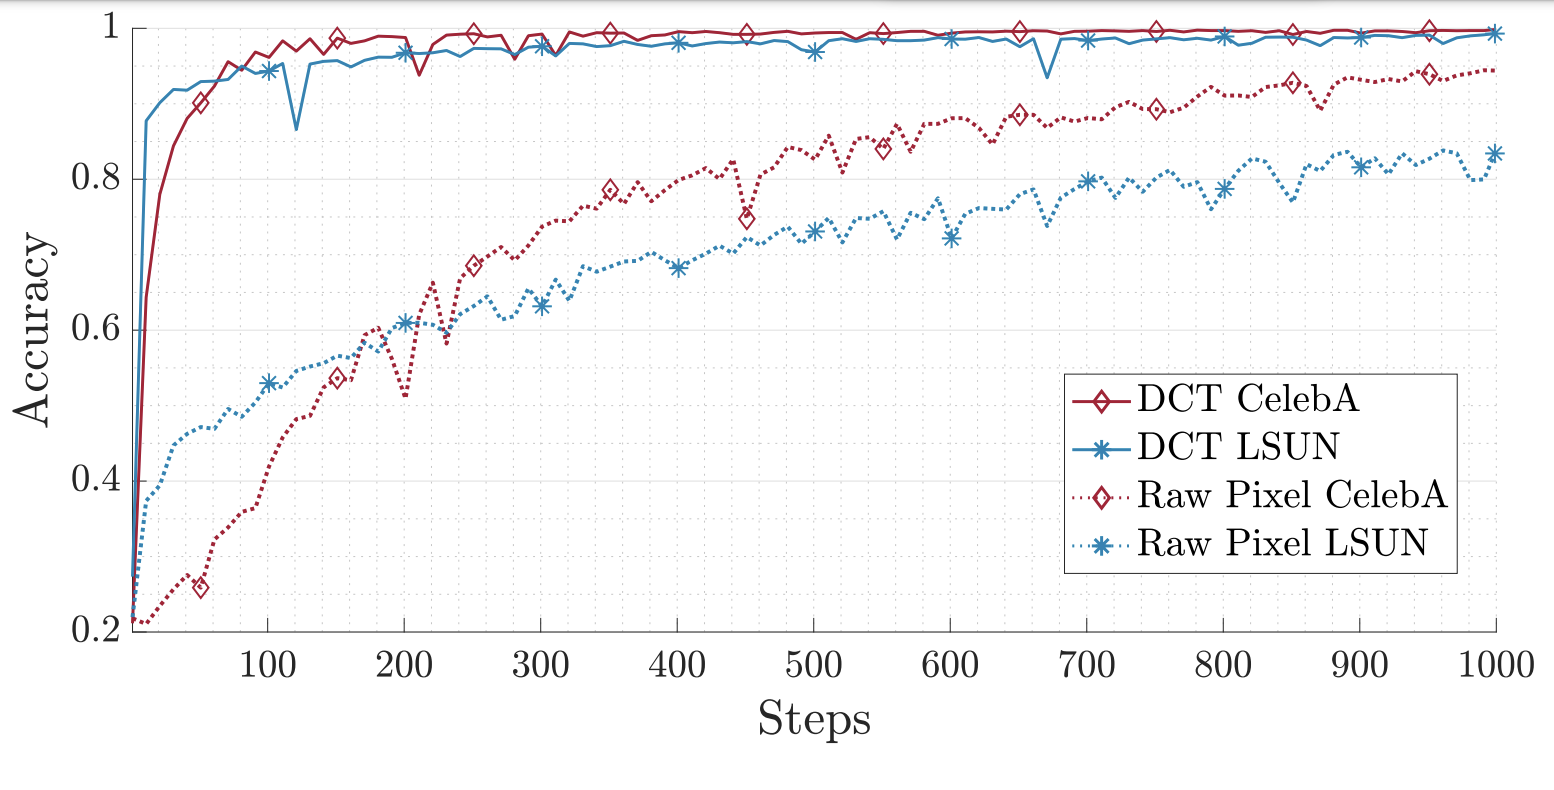
\includegraphics[width=1.0\linewidth]{Images/frank-acc-comparison-1.png}
	\begin{minipage}{0.9\linewidth}
		\caption{Đường cong độ chính xác theo bước huấn luyện. \textit{Nguồn: \cite{Frank2020LeveragingFA}}}
		\label{fig:frank-acc-comparison-1}
	\end{minipage}
\end{figure}\\
%
%
%
\textbf{Phương pháp F3-Net}~\cite{Qian2020ThinkingIF} (Hình~\ref{fig:model-f3-net-1}) do Qian đề xuất năm 2020.
Phương pháp này tập trung phân tích, rút trích các đặc trưng giả mạo trên miền tần số tại các khu vực cục bộ trên ảnh thông qua hai khối, \textit{Frequency-aware Decomposition (FAD)} và \textit{Local Frequency Statistics (LFS)}. FAD có chức năng phân rã $1$ ảnh đầu vào thành $N=3$ ảnh đầu ra, mỗi ảnh mang thông tin về phổ tần số khác nhau. LFS có chức năng tạo một mặt nạ thể hiện thống kê tần số cục bộ có tương quan không gian với ảnh đầu vào.
\begin{figure}[h]
	\centering
	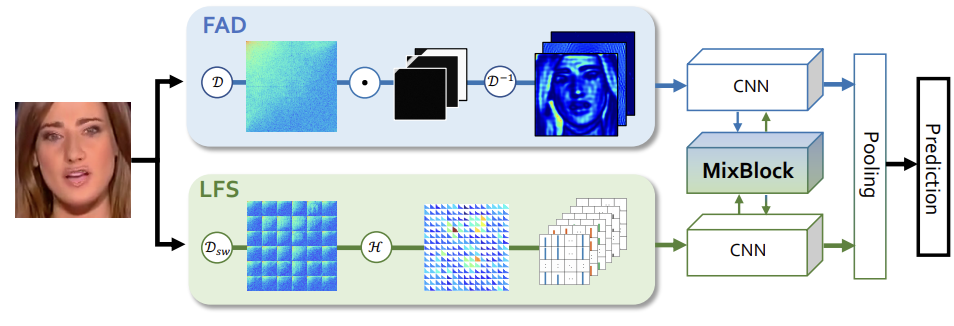
\includegraphics[width=1.0\linewidth]{Images/model-f3-net-1.png}
	\begin{minipage}{0.9\linewidth}
		\caption{Mô tả kiến trúc F3-Net. \textit{Nguồn: \cite{Qian2020ThinkingIF}}}
		\label{fig:model-f3-net-1}
	\end{minipage}
\end{figure}\\
%
%
-\textbf{Ưu điểm của phương pháp:}
%
Qian thực hiện phân tích tần số trên những khu vực ảnh cục bộ và biểu diễn lại các vị trí này trên ma trận, nhờ đó giữ được mối tương quan về không gian, đảm bảo tương thích với kiến trúc CNN~\cite{Krizhevsky2012ImageNetCW}. Cách làm này nhằm bổ sung khuyết điểm mất thông tin về không gian khi thực hiện biến đổi ảnh sang miền tần số.\\
%
%
-\textbf{Hạn chế của phương pháp:}
%
Các biến đổi sang miền tần số trên những khu vực ảnh nhỏ sẽ bị hạng chế về dải tần số, hơn nữa tại biên của các khu vực nhỏ này sẽ xuất hiện hiệu ứng rò rỉ (spectral leakage~\cite{ni_spectral_leakage}), sinh ra các tín hiệu nhiễu tần số cao, gây bất lợi cho quá trình huấn luyện.\\
%
%
\textbf{Phương pháp BiHPF}~\cite{Jeong2021BiHPFBH} của Jeong (2021).
%
Trong nghiên cứ này tác giả đề xuất bộ lọc thông cao song phương BiHPF với đầu vào là một biến đổi \gls{fft}~\cite{Arunachalam2013TheFF} của hình ảnh, giúp khuếch đại ảnh hưởng của các dấu hiệu tạo tác trong miền tần số.

Để phân tích, tìm ra các thành phần tần số đặc trưng có trong ảnh tạo sinh, Jeong thiết kế và huấn luyện một mô-đun tên là \textit{Artifact Compression Map}, có khả năng tách biệt các thành phần tần số đặc trưng của ảnh tạo sinh. Từ đó rút ra kết luận \textit{"Các dấu vết tạo tác xuất hiện chủ yếu trong các thành phần tần số cao và vùng nền của hình ảnh ở mức độ điểm ảnh"}. Nói cách khác, việc phân tích phổ tần số cao của các vùng ảnh có kết cấu đơn giản, bằng phẳng sẽ đem lại hiệu quả cao hơn trong nhiệm vụ phát hiện ảnh tạo sinh.

Do đó, BiHPF được thiết kế để trích xuất các dấu vết tạo tác có trong ảnh giả mạo trên miền tần số, tại các vùng ảnh bằng phẳng. Đầu ra của bộ lọc này sau đó cho qua bộ phân loại sử dụng kiến trúc Resnet50~\cite{He2015DeepRL}. thực hiện nhiệm vụ phát hiện ảnh tạo sinh.\\
%
-\textbf{Đóng góp của phương pháp:}
Đưa ra được bằng chứng \textit{"Các dấu vết tạo tác xuất hiện chủ yếu trong các thành phần tần số cao và vùng nền của hình ảnh ở mức độ điểm ảnh"}, cung cấp thông tin hữu ích cho nhiều nghiên cứu.\\
%
-\textbf{Hạn chế của phương pháp:}
Quá trình huấn luyện phức tạp. 
%
\textbf{Phương pháp FrePGAN}~\cite{Jeong2022FrePGANRD} được Jeong giới thiệu vào năm 2022.\\
Thông qua phân tích phổ tần số giữa ảnh thật và tạo sinh, tác giả phát hiện sự gia tăng năng phổ lượng đáng kể ở vùng tần số cao trong ảnh giả mạo, các dấu hiệu này dễ dàng quan sát được bằng mắt thường (Hình~\ref{fig:freqgan-power-spectrum-1}).
%
\begin{figure}[h]
	\centering
	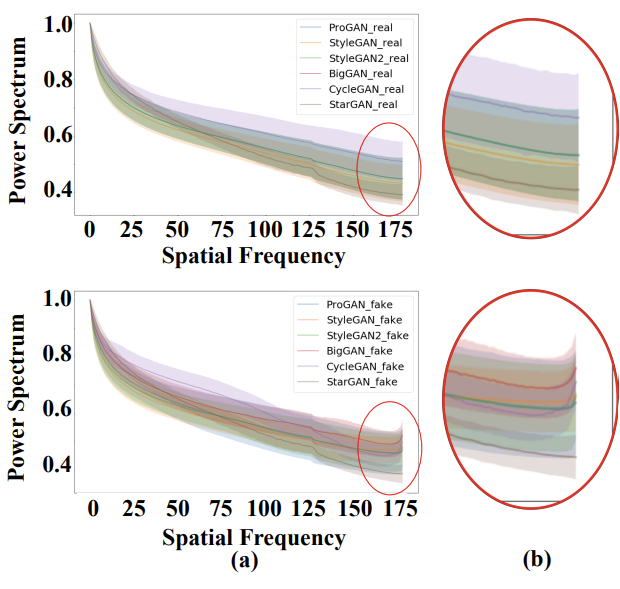
\includegraphics[width=0.7\linewidth]{Images/freqgan-power-spectrum-1.png}
	\begin{minipage}{0.9\linewidth}
		\caption{So sánh phổ công suất của dữ liệu thực và dữ liệu tạo sinh. \textit{Nguồn: \cite{Jeong2022FrePGANRD}}}
		\label{fig:freqgan-power-spectrum-1}
	\end{minipage}
\end{figure}\\
%
Ngoài ra các phương pháp sử dụng miền tần số có xu hướng quá khớp trong quá trình huấn luyện. Để khắc phục các hạn chế này, phương pháp FrePGAN sẽ tạo ra một bản đồ nhiễu trong miền tần số và đưa vào trong hình ảnh với mục đích tạo ra các mẫu dữ liệu khó, từ đó giúp mô hình tập trung tìm kiếm nhiều đặc trưng hữu ích hơn. 
%
-\textbf{Ưu điểm của phương pháp:} Huấn luyện một mạng GAN~\cite{Goodfellow2014GenerativeAN} có khả năng sinh ra các nhiễu loạn ở mức tần số, từ đó khuyến khích mô hình phân loại học thêm nhiều đặc trưng mới, làm tăng khả năng khái quát của mô hình.\\
-\textbf{Hạn chế của phương pháp:} Đào tạo mạng GAN~\cite{Goodfellow2014GenerativeAN} sinh nhiễu là phức tạp và khó kiểm soát. Hơn nữa thêm nhiễu vào dữ liệu tuy sẽ tăng tính khái quát của mô hình nhưng đồng thời cũng có xu hướng làm giảm độ chính xác.
%
%
%
\subsection{Nhóm phương pháp hỗn hợp}
Hướng tiếp cận này là sự kết hợp của nhiều phương pháp hoặc nhiều loại mô hình với nhau.\\
%
\textbf{Li và cộng sự (2024) đã công bố phương pháp SAFE~\cite{li2024improving}:}
%
Tác giả đã thực hiện nhiều kỹ thuật tăng cường dữ liệu bao gồm: ngẫu nhiên thay đổi các thuộc tính màu sắc, xoay, tạo ra mặt nạ ngẫu nhiên che khuất một phần hình ảnh, trước khi thực hiện trích xuất đặc trưng tần số cao trên miền tần số. Các bước thực hiện được minh hoạ ở Hình ~\ref{fig:model-SAFE-1}. 
%	
\begin{figure}[ht]
	\centering
	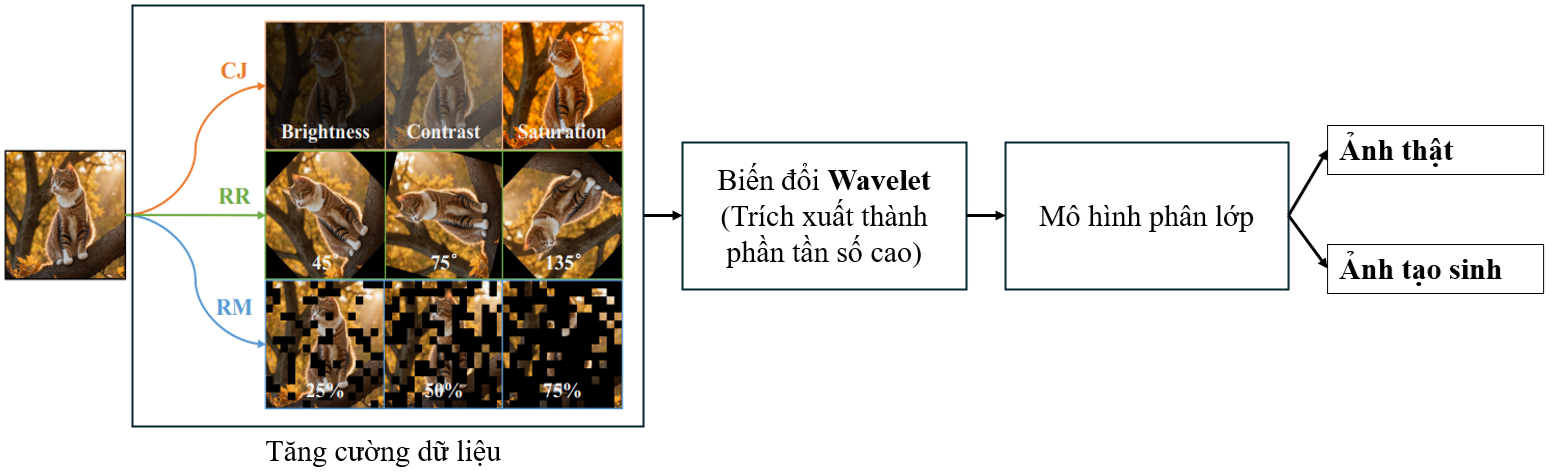
\includegraphics[width=1.0\linewidth]{Images/model-SAFE-1.png}	\begin{minipage}{0.9\linewidth}
		\caption{Mô tả phương pháp SAFE~\cite{li2024improving}.}
		\label{fig:model-SAFE-1}
	\end{minipage}
\end{figure}\\
%
%
%
-\textbf{Đóng góp của phương pháp:}
%
Li kết quả của nghiên cứu đã chứng tỏ ảnh hưởng tích cực của các kỹ thuật tăng cường dữ liệu đến tính khái quát của mô hình phân loại.

Ngoài ra tác giả cũng làm thực nghiệm để kiểm chứng mối tương quan cục bộ mạnh giữa các điểm ảnh kề nhau trong ảnh tạo sinh, được cho là gây ra bởi việc sử dụng toán tử \gls{up-sampling} và \gls{convolution} trong các mô hình tạo sinh.
%

%








\chapter{PHƯƠNG PHÁP ĐỀ XUẤT}
%https://ir.vnulib.edu.vn/bitstream/VNUHCM/32505/2/LeMinhHung.html
% Nhớ thêm trích dẫn tham khảo từ luận văn này (tham khảo về cách trình bày)
\label{Chapter3}
\section{Thử nghiệm sơ bộ và tìm hướng tiếp cận}
%
\subsection{Thử nghiệm 1}
%
\begin{figure}[ht!]
	\centering
	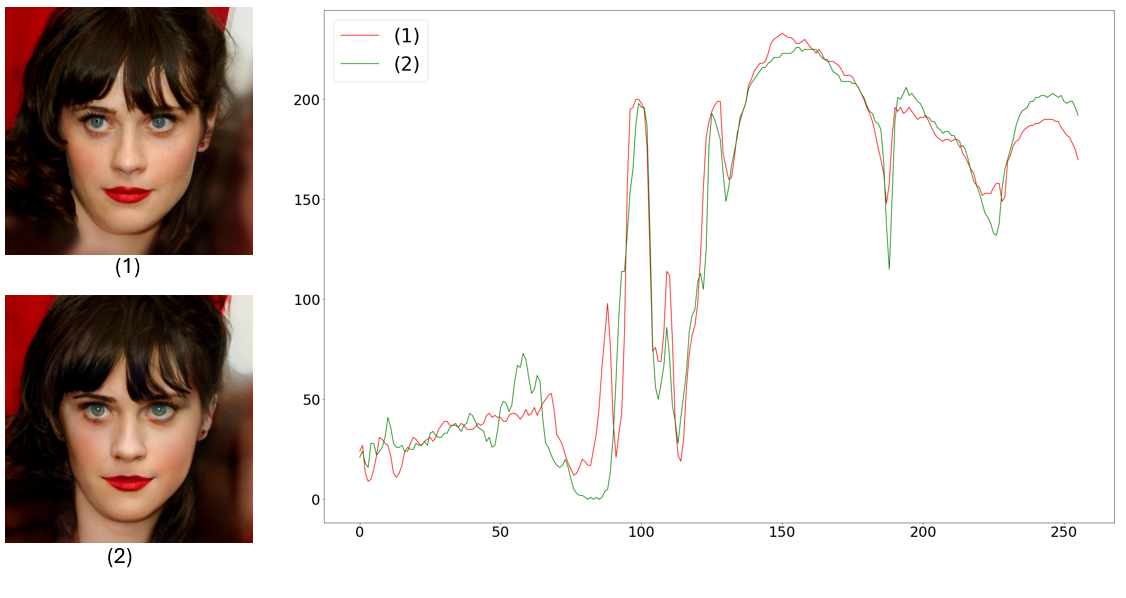
\includegraphics[width=1.0\linewidth]{Images/restyle-encoder-1.png}
	\begin{minipage}{1.0\linewidth}
		\caption{Biểu đồ (\textit{phải}) thể hiện mức xám dòng thứ 100 của ảnh thật (1) và ảnh tạo sinh (2).}
		\label{fig:restyle-encoder-1}
	\end{minipage}
\end{figure}
%
Trong Hình~\ref{fig:restyle-encoder-1}, ta sử dụng ảnh thật (1) lấy từ tập dữ liệu FFHQ và tạo ảnh giả tương ứng (2) bằng phương pháp ReStyle~\cite{alaluf2021restyle}. 
%
Việc sử dụng cặp ảnh thật–giả có cùng đặc điểm khuôn mặt giúp ta khảo sát trực quan độ khó của nhiệm vụ phân biệt hình ảnh tạo sinh. Kết quả cho thấy hai ảnh có mức độ tương đồng cao về hình dáng và chi tiết, gây khó khăn cho việc phân biệt bằng mắt thường.
%
Điều này có thể lý giải bởi thực tế rằng thị giác con người chủ yếu nhận biết thông tin ở các vùng ảnh có kích thước lớn và có độ tương phản cao, trong khi các khác biệt đặc trưng để phân biệt ảnh thật và ảnh tạo sinh rất có thể tồn tại ở mức độ điểm ảnh.
%
%

Các nghiên cứu trước đây \textcolor{red}{trích dẫn} cũng chỉ ra rằng các đặc trưng nhân tạo có xu hướng tập trung ở vùng tần số cao. Một số phương pháp đã tận dụng điều này để phát triển bộ phân loại dựa trên đặc trưng tần số \textcolor{red}{trích dẫn}.Phần~\ref{ssec:thu_nghiem_2}, ta tiến hành thử nghiệm nhằm đánh giá sự ảnh hưởng của đặc trưng tần số đến hiệu xuất bộ phân loại ảnh thật, giả.

\subsection{Thử nghiệm 2}
\label{ssec:thu_nghiem_2}
Bước tiếp theo của quá trình phân tích, ta thực hiện huấn luyện hai bộ phân loại dựa trên kiến trúc ResNet~\cite{He2015DeepRL} và sử dụng cùng bộ dữ liệu \textcolor{red}{[Tên tập dữ liệu]}.

\textbf{Bộ phân loại số 1:} (Original RGB ) ảnh đầu vào là ảnh màu RGB gốc, giữ nguyên toàn bộ thông tin tần số.  

\textbf{Bộ phân loại số 2:} (Highpass 50\%) Mô hình này sử dụng cùng kiến trúc với Bộ phân loại số 1, tuy nhiên ảnh đầu vào đã được xử lý bằng bộ lọc thông cao, trong đó 50\% thành phần tần số thấp đã bị loại bỏ thông qua biến đổi Fourier. Kết quả huấn luyện được trình bày trong Hình~\ref{fig:Experiment_Highpass50_percent}

%
\begin{figure}[ht!]
	\centering
	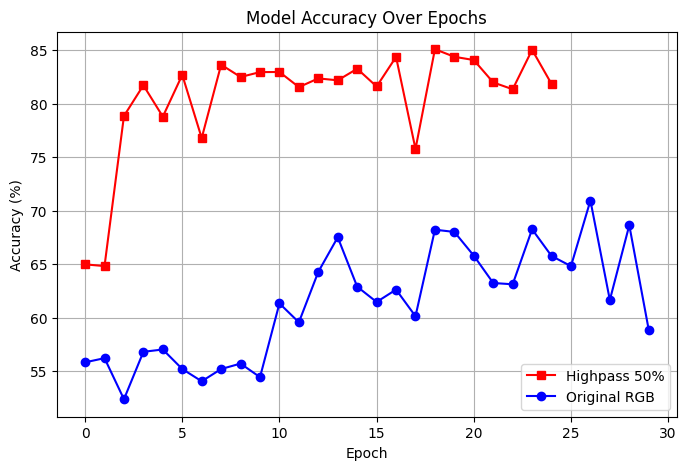
\includegraphics[width=1.0\linewidth]{Images/Experiment_Highpass50_percent.png}
	\begin{minipage}{1.0\linewidth}
		\caption{Độ chính xác của hai bộ phân loại trên tập kiểm tra trong quá trình huấn luyện.}
		\label{fig:Experiment_Highpass50_percent}
	\end{minipage}
\end{figure}

%
Thử nghiệm đã cho thấy các thành phần tần số cao đóng vai trò quan trọng trong quá trình phân loại ảnh thật – giả. Cụ thể, mô hình được huấn luyện trên ảnh đã qua bộ lọc thông cao (Highpass 50\%) đạt độ chính xác cao hơn so với mô hình sử dụng ảnh RGB gốc. Điều này gợi ý rằng thông tin tần số cao chứa các đặc trưng quan trọng giúp phân biệt ảnh giả mạo, trong khi các thành phần tần số thấp có thể chứa nhiều thông tin nền không hữu ích cho quá trình nhận diện.  

\subsection*{Mở rộng thử nghiệm với các mức lọc tần số cao khác nhau}

Nhằm đánh giá thêm tác động của các thành phần tần số cao trong việc phân loại ảnh thật và giả, chúng tôi tiếp tục mở rộng thử nghiệm với các mức lọc thông cao khác nhau: 60\%, 70\%, 80\%, và 90\%. Bằng cách này, ta có thể đánh giá ảnh hưởng của các tín hiệu tần số cao đến hiệu xuất của bộ phân loại.

Những quan sát từ thử nghiệm cho thấy rằng việc tăng cường khai thác thông tin ở dải tần số cao có thể mang lại lợi ích đáng kể cho nhiệm vụ phát hiện ảnh tạo sinh. Do đó, \textbf{hướng tiếp cận nghiên cứu trong phần tiếp theo sẽ tập trung vào khai thác đặc trưng tần số cao để cải thiện độ chính xác phân loại.}

\subsection{Các hạn chế khi dùng biến đổi Fourier}

Trong quá trình thử nghiệm, ta đã sử dụng phép biến đổi Fourier nhanh (FFT) để phân tích tín hiệu trong miền tần số và thực hiện việc loại bỏ các thành phần tần số thấp nhằm tập trung khai thác đặc trưng tần số cao. Việc này giúp tăng hiệu quả phân loại ảnh thật và giả mạo. Tuy nhiên, mặc dù FFT có ưu điểm về tốc độ tính toán nhanh hơn nhiều so với biến đổi Fourier rời rạc (DFT), quá trình áp dụng FFT và cắt lọc tần số cũng tồn tại những hạn chế nhất định.

\begin{itemize}
	\item Tuy độ phức tạp tính toán chỉ là $O(N\log{N})$ nhưng ta phải thêm bước biến đổi ngược (iFFT) về không gian ảnh ban đầu sau khi áp dụng mặt nạ lọc tần số.
	\item Khó khăn trong việc tối ưu hoá tốc độ bằng tính toán song song tận dụng sức mạnh của GPU.
	\item Tốn nhiều tài nguyên bộ nhớ do các biến đổi ở dạng số phức nên yêu cầu thêm bộ nhớ.
	\item Hiệu ứng biên trong biến đổi FFT làm xuất hiện các tín hiệu nhiễu không mong muốn.
\end{itemize}

\section{Biến đổi sai phân như một phép lọc thông cao: Phân tích từ góc nhìn miền tần số}

Để khắc phục các hạn chế của FFT trong việc lọc tần số cao, một hướng tiếp cận thay thế là xây dựng bộ lọc thông cao trực tiếp trong miền không gian ảnh, cho phép loại bỏ thành phần tần số thấp mà không cần thực hiện biến đổi FFT và biến đổi FFT ngược.
%
Cách làm này không chỉ giúp giảm độ phức tạp tính toán mà còn phù hợp hơn cho các hệ thống yêu cầu xử lý nhanh, có tài nguyên hạn chế hoặc dễ dàng tính toán song song nếu hệ thống hổ trợ GPU.

Trong phần này, tôi sẽ trình bày cơ sở lý thuyết của phương pháp xây dựng bộ lọc thông cao dựa trên việc biến đổi từ một bộ lọc thông thấp đơn giản – cụ thể là bộ lọc trung bình. 
%
Thông qua phân tích đáp ứng tần số, ta sẽ chứng minh rằng thao tác lấy sai phân (hiệu) giữa các điểm ảnh kề nhau có thể được xem như một phép lọc thông cao hiệu quả, với độ phức tạp rất thấp.

\subsection{Bộ Lọc Trung Bình (Low-Pass Filter)}

Bộ lọc trung bình rời rạc \( h_{\mathrm{LP}}[n] \) có thể được định nghĩa theo công thức:

\[
h[n] =
\begin{cases}
	\frac{1}{M}, & 0 \leq n < M \\
	0, & \text{ngược lại}
\end{cases}
\]

Trong đó, \( M \) là kích thước của cửa sổ trượt. Tín hiệu đầu ra của bộ lọc trung bình được tính bằng:

\[
y_{\mathrm{LP}}[n] = \frac{1}{M} \sum_{k=0}^{M-1} x[n-k]
\]

Để tìm đáp ứng tần số, ta tiến hành biến đổi Fourier rời rạc của bộ lọc:

\[
H_{\mathrm{LP}}(\omega) = \sum_{n=0}^{M-1} \frac{1}{M} e^{-j \omega n} = \frac{1}{M} \cdot \frac{1 - e^{-j M \omega}}{1 - e^{-j \omega}}
\]

Biểu thức này có thể được rút gọn thành:

\[
H_{\mathrm{LP}}(\omega) = \frac{1}{M} e^{-j \omega \frac{M-1}{2}} \cdot \frac{\sin\left(\frac{M \omega}{2}\right)}{\sin\left(\frac{\omega}{2}\right)}
\]

Với biên độ đáp ứng tần số là:

\[
|H_{\mathrm{LP}}(\omega)| = \left| \frac{1}{M} \cdot \frac{\sin\left( \frac{M \omega}{2} \right)}{\sin\left( \frac{\omega}{2} \right)} \right|
\]

\subsection*{Phân Tích Đặc Tính Đáp Ứng Biên Độ}

- Khi \( \omega \to 0 \), theo định lý L'Hopital, ta có:

\[
\lim_{\omega \to 0} |H_{\mathrm{LP}}(\omega)| = 1
\]

- Khi \( \omega \to \pi \), kết quả phụ thuộc vào giá trị của \( M \):

- Với \( M \) chẵn:

\[
\sin\left(\frac{M\pi}{2}\right) = 0 \Rightarrow |H_{\mathrm{LP}}(\pi)| = 0
\]

- Với \( M \) lẻ:

\[
\sin\left(\frac{M\pi}{2}\right) = \pm 1 \Rightarrow |H_{\mathrm{LP}}(\pi)| = \frac{1}{M}
\]

**Nhận xét** Để triệt tiêu hoàn toàn tần số cao, ta nên chọn \( M \) chẵn.

\subsection*{Thiết Kế Bộ Lọc Thông Cao (High-Pass Filter)}

Bộ lọc thông cao có thể được xây dựng từ bộ lọc thông thấp thông qua một quan hệ tuyến tính. Cụ thể, tín hiệu đầu ra của bộ lọc thông cao là:

\[
y_{\mathrm{HP}}[n] = x[n] - y_{\mathrm{LP}}[n]
\]

Với \( h_{\mathrm{HP}}[n] \) là đáp ứng xung của bộ lọc thông cao, ta có:

\[
h_{\mathrm{HP}}[n] = \delta[n] - h_{\mathrm{LP}}[n]
\]

Đáp ứng tần số của bộ lọc thông cao được cho bởi:

\[
H_{\mathrm{HP}}(\omega) = 1 - H_{\mathrm{LP}}(\omega)
\]

Thay thế biểu thức của \( H_{\mathrm{LP}}(\omega) \), ta có:

\[
H_{\mathrm{HP}}(\omega) = 1 - \frac{1}{M} e^{-j \omega \frac{M-1}{2}} \cdot \frac{\sin\left(\frac{M \omega}{2}\right)}{\sin\left(\frac{\omega}{2}\right)}
\]

Biên độ đáp ứng tần số của bộ lọc thông cao là:

\[
|H_{\mathrm{HP}}(\omega)| = \left| 1 - \frac{1}{M} \cdot \frac{\sin\left( \frac{M \omega}{2} \right)}{\sin\left( \frac{\omega}{2} \right)} \right|
\]

\subsection*{Phân Tích Đặc Tính Đáp Ứng Biên Độ}

\begin{itemize}
	\item Khi \( \omega \to 0 \):
	\[
	|H_{\mathrm{HP}}(0)| = |1 - H(0)| = 0
	\]
	
	\item Khi \( \omega \to \pi \), kết quả cũng phụ thuộc vào giá trị của \( M \):
	
	Với \( M \) chẵn:
	
	\[
	|H_{\mathrm{HP}}(\pi)| = 1 - 0 = 1, \quad \text{toàn bộ tần số cao nhất được bảo toàn}
	\]
	
	Với \( M \) lẻ:
	
	\[
	|H_{\mathrm{HP}}(\pi)| = 1 - \frac{1}{M} < 1, \quad \text{một phần tần số cao nhất bị suy hao}
	\]
\end{itemize}



**Nhận xét:** Để giữ lại tần số cao nhiều nhất, ta nên chọn \( M \) chẵn.

\subsection*{Cửa Sổ Bộ Lọc Thông Cao}
\label{sec:cua_so_loc_thong_cao}

Từ biểu thức đáp Ứng Xung của Bộ Lọc Thông Cao:

\[
h_{\mathrm{HP}}[n] = \delta[n] - h_{\mathrm{LP}}[n]
\]

Với \( n = 0 \):

\[
h_{\mathrm{HP}}[0] = \delta[0] - h_{\mathrm{LP}}[0] = 1 - \frac{1}{M}
\]

Với \( 1 \leq n < M \):

\[
h_{\mathrm{HP}}[n] = \delta[n] - \frac{1}{M} = 0 - \frac{1}{M} = -\frac{1}{M}
\]

Với \( n \geq M \):

\[
h_{\mathrm{HP}}[n] = \delta[n] - 0 = 0
\]

Do đó, đáp ứng xung của bộ lọc thông cao có dạng:

\[
h_{\mathrm{HP}}[n] =
\begin{cases}
	1 - \frac{1}{M}, & n = 0 \\
	-\frac{1}{M}, & 1 \leq n < M \\
	0, & \text{ngược lại}
\end{cases}
\]

Biểu thức tổng quát cho bộ lọc thông cao có thể được diễn đạt dưới dạng vector độ dài \( M \):

\begin{equation}
	\label{eq:h_HP}
	h_{\mathrm{HP}}[n] = \left[ 1 - \frac{1}{M},\ -\frac{1}{M},\ -\frac{1}{M},\ \ldots,\ -\frac{1}{M} \right]
\end{equation}
%

Bộ lọc thông cao có thể được xây dựng từ bộ lọc trung bình thông qua một phép toán đơn giản. Qua thực nghiệm, ta thấy rằng \( M = 2 \) cho kết quả tối ưu cho mô hình.
%
%
\section{Xây dựng khối tiền xử lý dựa trên bộ lọc thông cao}
Phương trình~\eqref{eq:h_HP} mô tả bộ lọc thông cao dưới dạng tổng quát. Ta mở rộng thành ma trận $H_x, H_y$ như bên dưới để thuận tiện cho việc sử dụng thư viện như \texttt{Pytorch} khi lập trình.
	\[
	H_x = \begin{bmatrix}
		0 & 0 & 0 \\
		0 & \tfrac{1}{2} &  \text{-}\tfrac{1}{2} \\
		0 & 0 & 0
	\end{bmatrix} \qquad \qquad
	H_y = \begin{bmatrix}
		0 & 0 & 0 \\
		0 & \tfrac{1}{2} &  0 \\
		0 & \text{-}\tfrac{1}{2} & 0
	\end{bmatrix}
	\]
	
Dựa trên phân tích tại mục \ref{sec:cua_so_loc_thong_cao}, ta chọn độ dài cửa sổ lọc $M=2$ vì giá trị $M$ chẵn giữ lại vùng tần số cao tốt hơn so với giá trị lẻ. Đồng thời, lựa chọn $M$ nhỏ giúp giảm chi phí tính toán.

\section{Mô hình đề xuất}

Trong đề tài này, mục tiêu hướng đến là xây dựng một phương pháp có cấu trúc đơn giản, tối ưu về tốc độ xử lý, và phù hợp với các hệ thống có tài nguyên hạn chế trong nhiệm vụ phát hiện hình ảnh tạo sinh. Để đạt được mục tiêu này, kiến trúc ResNet~\cite{He2015DeepRL} được lựa chọn làm nền tảng cho mô hình phân loại.

ResNet~\cite{He2015DeepRL} là một trong những kiến trúc \textcolor{red}{CNN} hiệu quả nhất được đề xuất bởi He et al. (2015), nổi bật nhờ cơ chế \textcolor{red}{skip connection}, cơ chế này cho phép huấn luyện các mô hình có chiều sâu lớn hơn mà vẫn duy trì hiệu quả hội tụ, đồng thời hạn chế hiện tượng mất mát thông tin trong quá trình lan truyền ngược.

So với các kiến trúc phức tạp hơn như EfficientNet~\cite{zhong2024patchcraftexploringtexturepatch}, Vision Transformer~\cite{dosovitskiy2020image}, ResNet có ưu điểm là dễ triển khai, ít tham số hơn, và có thể tùy chỉnh dễ dàng số lượng tầng để phù hợp với yêu cầu tính toán của hệ thống. Trong phạm vi nghiên cứu này, một phiên bản rút gọn từ ResNet-50~\cite{He2015DeepRL} được sử dụng nhằm đảm bảo cân bằng giữa độ chính xác và chi phí tính toán.

Bên cạnh đó, ResNet~\cite{He2015DeepRL} cũng cho thấy khả năng trích xuất đặc trưng tốt ở các tác vụ phân biệt hình ảnh có sai khác nhỏ, chẳng hạn như sự khác biệt vi mô giữa ảnh thật và ảnh tạo sinh – điều này đặc biệt quan trọng trong bối cảnh deepfake ngày càng tinh vi.

\subsection{Kiến trúc mô hình rút gọn từ ResNet-50}
\label{sec:kien_truc_mo_hinh_rut_gon_tu_resnet_50}
Mô hình đề xuất được mô tả trong Hình~\ref{fig:figure_model_architecture}), trong đó chỉ sử dụng hai khối residual đầu tiên của kiến trúc ResNet-50 (tương ứng với \texttt{Layer1} và \texttt{Layer2}) để thực hiện trích xuất đặc trưng, kết hợp với một bộ phân loại nhị phân đơn giản ở đầu ra. Việc tinh giản này giúp giảm số lượng tham số từ khoảng 23 triệu (của ResNet-50 đầy đủ) xuống còn khoảng 1.4 triệu tham số. Mô hình bao gồm các thành phần chính như sau:
%
\begin{figure}[ht!]
	\centering
	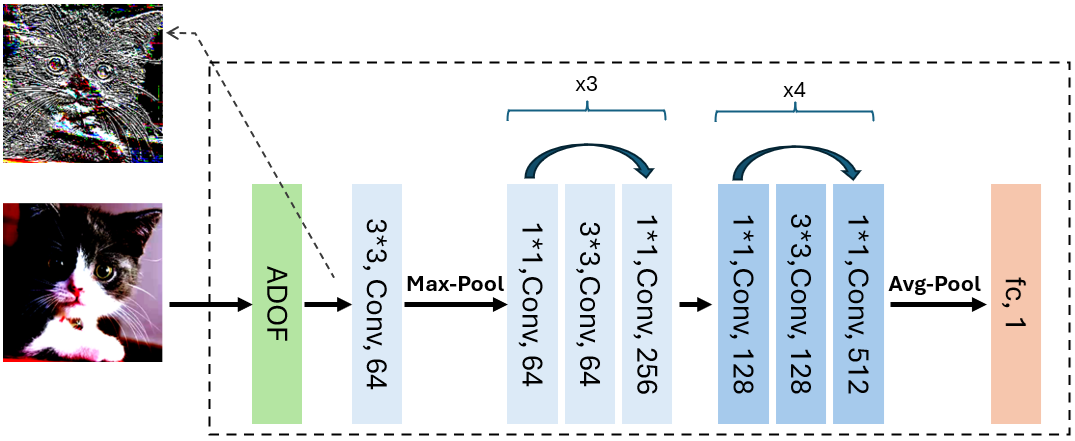
\includegraphics[width=1.0\linewidth]{Images/figure_model_architecture.png}
	\begin{minipage}{1.0\linewidth}
		\vspace{5mm}
		\caption{Kiến trúc mạng Resnet-50 rút gọn}
		\label{fig:figure_model_architecture}
	\end{minipage}
\end{figure}
%
%

\begin{itemize}
	\item \textbf{Khối tiền xử lý ADOF}
	
	Phương trình~\eqref{eq:h_HP} mô tả bộ lọc thông cao dưới dạng tổng quát. Ta mở rộng thành ma trận $H_x, H_y$ như bên dưới để thuận tiện cho việc sử dụng thư viện như \texttt{Pytorch} khi lập trình.
	\[
		H_x = \begin{bmatrix}
			0 & 0 & 0 \\
			0 & \tfrac{1}{2} &  \text{-}\tfrac{1}{2} \\
			0 & 0 & 0
		\end{bmatrix} \qquad \qquad
		H_y = \begin{bmatrix}
			0 & 0 & 0 \\
			0 & \tfrac{1}{2} &  0 \\
			0 & \text{-}\tfrac{1}{2} & 0
		\end{bmatrix}
	\]
	
	\begin{itemize}
		\item Hai 2 bộ lọc thông cao áp dụng cho 2 hướng $x, y$ giúp loại bỏ thông tin tần số thấp của hình ảnh.
		\item Đầu ra tương ứng của 2 bộ lọc thông cao được kết hợp với nhau để tạo ra một bản đồ đặt trưng. \textcolor{red}{Chi tiết được trình bài tại..}
	\end{itemize}
	\item \textbf{Tầng đầu vào (Stem Layer)}:
	\begin{itemize}
		\item Một lớp \texttt{convolution} với kernel \(3 \times 3\), stride = 1, padding = 1, tiếp theo là \texttt{Batch Normalization} và hàm kích hoạt \texttt{ReLU}.
		\item Một lớp Max Pooling với kernel \(3 \times 3\), stride = 2 nhằm giảm kích thước đầu vào.
	\end{itemize}
	
	\item \textbf{Khối Layer1}:
	\begin{itemize}
		\item Gồm 3 block dạng Bottleneck, sử dụng \textcolor{red}{\texttt{Skip connection}} để học các đặc trưng cơ bản như cạnh, vùng chuyển tiếp và kết cấu ảnh.
	\end{itemize}
	
	\item \textbf{Khối Layer2}:
	\begin{itemize}
		\item Gồm 4 khối \texttt{Bottleneck}, tiếp tục trích xuất đặc trưng ở mức trừu tượng cao hơn, giúp mô hình phân biệt được các khác biệt tinh vi giữa ảnh thật và ảnh tạo sinh.
	\end{itemize}
	
	\item \textbf{Bộ phân loại đầu ra}:
	\begin{itemize}
		\item Một lớp \texttt{Global Average Pooling} để chuyển đổi bản đồ đặc trưng thành vector đặc trưng cố định.
		\item Một lớp \texttt{Fully Connected} với một ngõ ra duy nhất, sử dụng hàm kích hoạt \texttt{sigmoid} để phân loại ảnh đầu vào là thật hay tạo sinh.
	\end{itemize}
\end{itemize}

\subsection{Quy trình huấn luyện và sử dụng}
%
\label{ssec:quy_trinh_huan_luyen}
%
Quá trình huấn luyện được mô tả trong Hình~\ref{fig:offline-training-process}, ảnh đầu vào sẽ được chuẩn hóa và tiền xử lý nhằm đồng nhất kích thước, tăng tính đa dạng qua các kỹ thuật tăng cường dữ liệu xoay và lật ảnh. Sau bước này, ảnh được đưa qua khối \textcolor{red}{ADOF} – có chức năng lọc lấy những tín hiệu ở tần số cao trong ảnh, nơi mà các mô hình tạo sinh thường để lại dấu vết.
%
\begin{figure}[ht!]
	\centering
	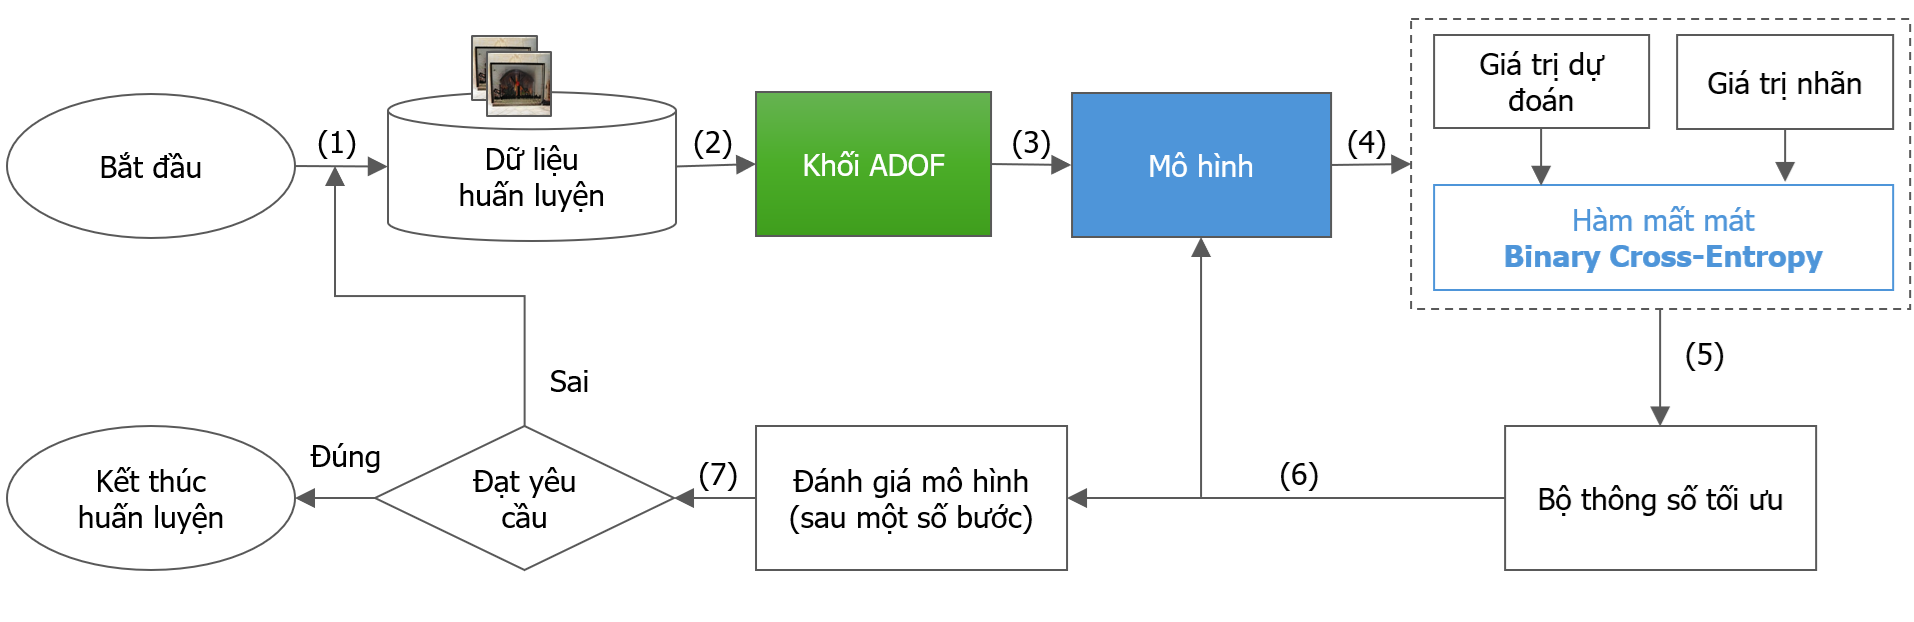
\includegraphics[width=1.0\linewidth]{Images/offline-training-process.png}
	\begin{minipage}{1.0\linewidth}
		\vspace{3mm}
		\caption{Quy trình huấn luyện}
		\label{fig:offline-training-process}
	\end{minipage}
\end{figure}
%
Đầu ra từ khối \textcolor{red}{ADOF} sau đó được đưa vào một kiến trúc ResNet-50~\cite{He2015DeepRL} đã được rút gọn và điều chỉnh nhằm trích xuất đặc trưng và thực hiện phân loại. Kiến trúc này được giảm bớt số lượng tầng so với phiên bản đầy đủ để giảm chi phí tính toán nhưng vẫn giữ lại khả năng biểu diễn cần thiết cho bài toán nhị phân. Đầu ra cuối cùng của mạng là một giá trị xác suất thể hiện mức độ tin tưởng rằng ảnh đầu vào là ảnh tạo sinh. Hàm mất mát được sử dụng trong quá trình huấn luyện là \textcolor{red}{Binary Cross-Entropy}, kết hợp với thuật toán tối ưu \textcolor{red}{Adam}. Sự lựa chọn này đặc biệt phù hợp với bài toán phân loại nhị phân, giúp mô hình hội tụ nhanh và ổn định. 

Quá trình huấn luyện được tổ chức thành nhiều bước cập nhật trọng số trong mỗi \textcolor{red}{epoch}. Mỗi bước tương ứng với một \textcolor{red}{batch} dữ liệu được đưa vào mô hình để tính toán hàm mất mát và cập nhật trọng số thông qua lan truyền ngược. Sau khi hoàn tất một \textcolor{red}{epoch} – tức là toàn bộ tập huấn luyện đã được xử lý – mô hình sẽ được đánh giá trên tập dữ liệu kiểm thử nhằm theo dõi hiệu năng tổng thể và điều chỉnh chiến lược huấn luyện nếu cần thiết. Quá trình này tiếp tục cho đến khi mô hình đạt đến số \textcolor{red}{epoch} tối đa đã định hoặc khi các chỉ số đánh giá dừng cải thiện trong một khoảng thời gian xác định trước. Quy trình huấn luyện như trên giúp mô hình học được các đặc trưng phân biệt hiệu quả giữa ảnh thật và ảnh tạo sinh, đồng thời hạn chế hiện tượng \textcolor{red}{overfitting}.
%
%
\begin{figure}[ht!]
	\centering
	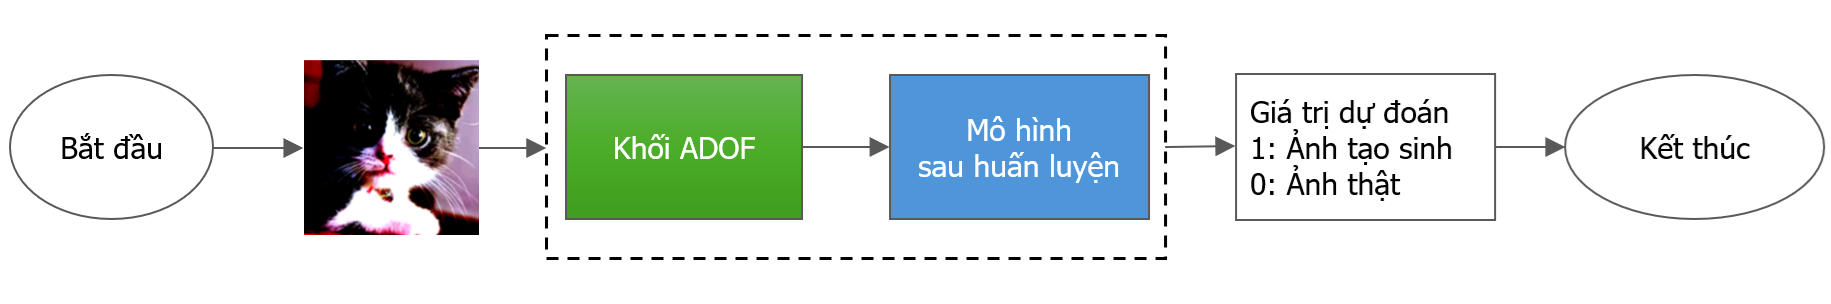
\includegraphics[width=1.0\linewidth]{Images/online-serving.png}
	\begin{minipage}{1.0\linewidth}
		\vspace{3mm}
		\caption{Quy trình sử dụng}
		\label{fig:online-serving}
	\end{minipage}
\end{figure}
%
%

Sau khi quá trình huấn luyện hoàn tất, mô hình đã sẵn sàng cho việc dự đoán trên dữ liệu mới (chi tiết được mô tả trong Hình~\ref{fig:online-serving}). Trong giai đoạn này, ảnh đầu vào sẽ được chuẩn hoá theo đúng các thông số đã sử dụng trong quá trình huấn luyện nhằm đảm bảo tính nhất quán về phân phối dữ liệu. Tiếp theo, ảnh được đưa qua khối \textcolor{red}{ADOF} để trích xuất các tín hiệu tần số cao. Đầu ra từ khối này được chuyển vào mô hình đã huấn luyện để thực hiện suy luận và đưa ra kết quả dự đoán cuối cùng.

\section{Tối giản mô hình với kỹ thuật Feature-Based Knowledge Distillation}

Nhằm tối ưu khả năng triển khai thực tế trên các thiết bị có tài nguyên hạn chế, sau khi hoàn tất huấn luyện mô hình với kiến trúc trình bày ở phần~\ref{sec:kien_truc_mo_hinh_rut_gon_tu_resnet_50}, ta tiếp tục áp dụng kỹ thuật \textcolor{red}{Feature-Based Knowledge Distillation} để rút gọn mô hình.

Cụ thể, mô hình đã huấn luyện sẽ đóng vai trò là mô hình Teacher, từ đó truyền đạt kiến thức cho một mô hình Student nhỏ gọn hơn. Thay vì chỉ dựa vào đầu ra cuối cùng, mô hình Student được hướng dẫn học theo các đặc trưng trung gian từ Teacher, giúp duy trì hiệu suất nhận dạng trong khi giảm đáng kể kích thước và chi phí suy luận của mô hình.

\subsection{Kiến trúc mô hình Student}
%figure_model_student_architecture.png
%
%
Trong mô hình Student, ta chỉ giữ lại một khối \texttt{Bottleneck} tại \texttt{Layer1} (thay vì ba khối) và một khối \texttt{Bottleneck} tại \texttt{Layer2} (thay vì bốn khối) từ mô hình Teacher (Hình~\ref{fig:figure_model_architecture}).
%
Việc lựa chọn số lượng \texttt{Layer} được giữ lại trong mô hình Student là kết quả của quá trình thử nghiệm thực tế, với tiêu chí cân bằng giữa độ chính xác và độ phức tạp của mô hình.

\subsection{Quy trình huấn luyện và sử dụng}
%offline-training-process-distillation.png
%
\begin{figure}[ht!]
	\centering
	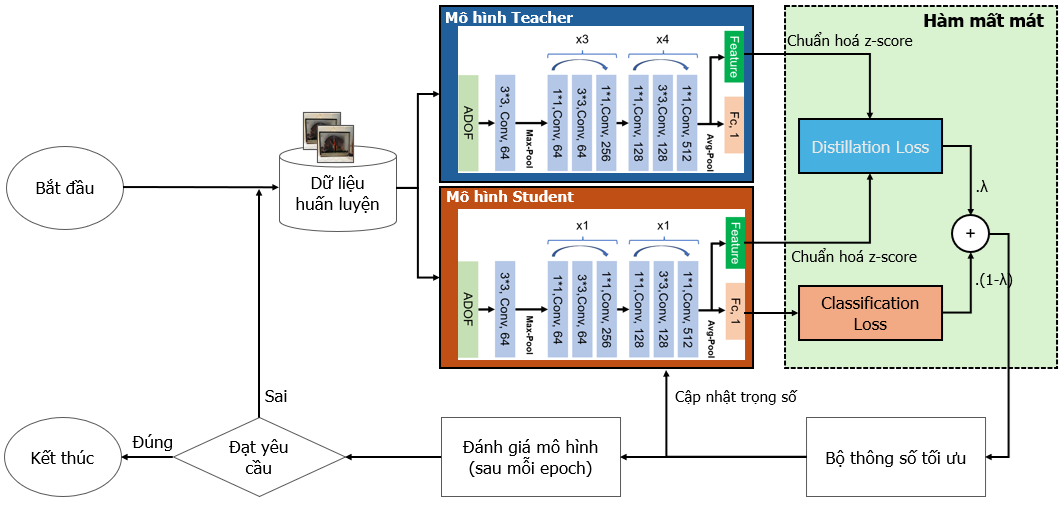
\includegraphics[width=1.0\linewidth]{Images/offline-training-process-distillation.png}
	\begin{minipage}{1.0\linewidth}
		\vspace{5mm}
		\caption{Quy trình huấn luyện mô hình áp dụng kỹ thuật Knowledge-Distillation}
		\label{fig:offline-training-process-distillation}
	\end{minipage}
\end{figure}
%
%
Quy trình huấn luyện trải qua các bước tương tự với như phần~\ref{ssec:quy_trinh_huan_luyen}.
%
Điểm khác biệt nằm ở quá trình lan truyền thuận, hàm mất mát và việc cập nhật bộ trọng số cho mô hình.
%
\begin{itemize}
	\item Lan truyền thuận: Hình ảnh từ đầu vào sẽ được đi qua cả hai mô hình Teacher và Student. Sau đó ta trích xuất véc-tơ đặc trưng ở đầu ra của \texttt{Layer2} trong mỗi mô hình và đưa vào hàm mất mát.
	
	\item  Hàm mất mát: Là sự kết hợp của 2 thành phần \textcolor{red}{Distillation} và \textcolor{red}{Binary Cross Entropy}, chi tiết được trình bày tại \textcolor{red}{tham chiều tới..}
	
	\item Cập nhật trọng số: Trong suốt quá trình huấn luyện, mô hình Teacher chỉ sử dụng duy nhất một bộ trọng số đã được huấn luyện trước. Việc cập nhật bộ trọng số chỉ được áp dụng cho mô hình Student.
\end{itemize}

Sau khi quá trình huấn luyện hoàn tất, mô hình Student đã sẵn sàng cho việc dự đoán trên dữ liệu mới (chi tiết xem trên Hình~\ref{fig:online-serving}). 









\chapter{THỰC NGHIỆM VÀ ĐÁNH GIÁ KẾT QUẢ}
\label{Chapter4}
\section{Chuẩn bị dữ liệu}
Luận văn sử dụng bộ dữ liệu \textbf{ForenSynths}~\cite{Wang2019CNNGeneratedIA} trong quá trình nghiên cứu và huấn luyện. Các hình ảnh thật được trích từ bộ dữ liệu LSUN~\cite{Yu2015ConstructionOA}, trong khi các hình ảnh giả mạo được tạo ra từ nhiều mô hình sinh ảnh khác nhau (ProGAN~\cite{karras2018progressive}, StyleGAN~\cite{karras2019style}, BigGAN~\cite{brock2018large}, CycleGAN~\cite{zhu2017unpaired}...). Chi tiết về bộ dữ liệu được thống kê trong Bảng~\ref{tab:forensynths-dataset}. Đây là bộ dữ liệu được nhiều nghiên cứu sử dụng cho nhiệm vụ phát hiện ảnh tạo sinh.

Ngoài bộ dữ liệu \textbf{ForenSynths}~\cite{Wang2019CNNGeneratedIA}, quá trình đánh giá mô hình được thực hiện trên các bộ dữ liệu khác nhau, giúp xác định tính khái quát của mô hình sau huấn luyện.

\subsection{Tập dữ liệu dùng cho quá trình huấn luyện mô hình}
Tập dữ liệu \textbf{ProGAN} thuộc bộ dữ liệu \textbf{ForenSynths}\cite{Wang2019CNNGeneratedIA} được sử dụng để huấn luyện mô hình. 
Cụ thể, tập dữ liệu có 20 danh mục đối tượng, trong đó có 18.000 hình ảnh thật được trích từ bộ dữ liệu LSUN~\cite{Yu2015LSUNCO}, 18.000 hình ảnh tạo sinh bằng mô hình \textbf{ProGAN}~\cite{karras2018progressive}. Trong luận văn này, bốn trong hai mươi danh mục đối tượng được lựa chọn để huấn luyện gồm: \textit{car}, \textit{cat}, \textit{chair}, và \textit{horse}. Việc lựa chọn các lớp này nhằm mục đích đảm bảo tính tương đồng với các nghiên cứu trước đây~\cite{trich_dan_bon_lop}, từ đó giúp thuận tiện hơn trong việc so sánh kết quả.
%
\begin{figure}[ht!]
	\centering
	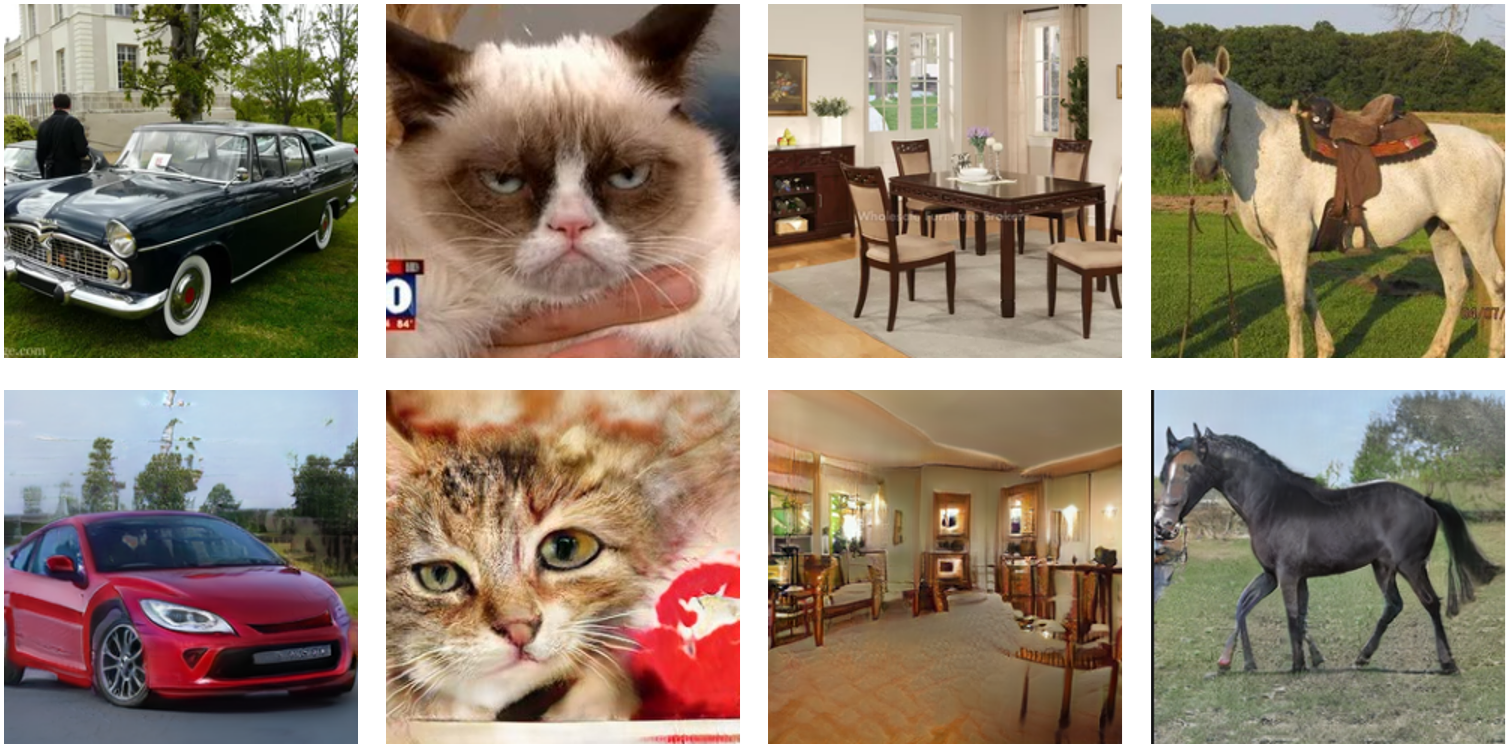
\includegraphics[width=1.0\linewidth]{Images/dataset_progan_samples.png}
	\begin{minipage}{1.0\linewidth}
		\vspace{5mm}
		\caption{Một vài hình ảnh trong tập dữ liệu huấn luyện (các hình ảnh thật ở hàng trên).}
		\label{fig:dataset_progan_samples}
	\end{minipage}
\end{figure}
%

\begin{table}[h]%[htbp]
	\scriptsize 
	\renewcommand{\arraystretch}{1.2} % Tăng chiều cao các hàng lên 1.5 lần
	\centering
	\caption{Tập dữ liệu Forensynths}
	\label{tab:forensynths-dataset}
	\begin{tabular}{|l|c|c|c|c|c|c|}
		\hline
		\textbf{Mô hình} & \textbf{Số lượng} & \textbf{Số danh mục} & \textbf{Tổng cộng} \\ \hline
		ProGAN & 18.000 & 20 & 360.000 \\ 
		StyleGAN  & 18.000 & 20 & 360.000 \\ 
		Stylegan2 & 18.000 & 20 & 360.000 \\  
		BigGAN & 18.000 & 20 & 360.000 \\  
		CycleGAN & 18.000 & 20 & 360.000 \\  
		StarGAN & 18.000 & 20 & 360.000 \\  
		GauGAN & 18.000 & 20 & 360.000 \\  
		Deepfake & 18.000 & 20 & 360.000 \\ 
		\hline
	\end{tabular}
\end{table}

%\vspace{-0.1cm} % Điều chỉnh khoảng cách nếu cần
%\textit{Tất cả hình ảnh trong {Bảng}~\ref{tab:forensynths-dataset} được định dạng (*.png), kích thước} (\( \mathit{256 \times 256 \times 3} \)).


\subsection{Tập dữ liệu dùng cho quá trình đánh giá mô hình}
Luận văn sử dụng các hình ảnh thật và hình ảnh giả mạo đến từ nhiều mô hình tạo sinh khác nhau nhằm đánh giá được tính khái quát của mô hình  (thông tin chi tiết xem Phụ lục~\ref{app:tables})
\begin{itemize}
	\item Tập dữ liệu \textbf{Self-Synthesis 9 GANs}~\cite{Tan2023RethinkingTU}, các hình ảnh giả mạo được thu thập từ 9 mô hình GAN~\cite{Goodfellow2014GenerativeAN} khác nhau. Tổng cộng gồm 36,000 hình ảnh, số lượng hình ảnh thật và giả mạo trong tập dữ liệu là ngang nhau.
	\item Tập dữ liệu \textbf{DiffusionForensics}~\cite{Wang2023DIREFD}, tác giả sử dụng 8 mô hình Diffusion~\cite{Ho2020DenoisingDP} khác nhau để sinh hình ảnh. Những mô hình này được huấn luyện trên tập ảnh LSUN-Bedroom~\cite{Yu2015LSUNCO} và ImageNet~\cite{5206848}, hình ảnh thật cũng được trích từ hai tập dữ liệu này. Tổng số lượng hình ảnh là 464,000, trong đó 50\% là hình ảnh thật (xem Bảng~\ref{tab:diffusionforensics_dataset}).
	%
	\item Tập dữ liệu \textbf{Ojha}~\cite{Ojha2023TowardsUF}, bao gồm 16,000 hình ảnh, trong đó các hình ảnh thật được trích xuất từ tập dữ liệu LAION~\cite{abs-2111-02114}, các hình ảnh giả được tạo từ nhiều mô hình Diffusion~\cite{Ho2020DenoisingDP} khác nhau, quá trình sinh ảnh sử dụng các câu mô tả hình ảnh thật tương ứng để cung cấp thông tin cho mô hình.
	%\item Tập kiểm tra 4
\end{itemize}

\textcolor{red}{Chi tiết của từng tập dữ liệu có thể xem ở phần phụ lục}

\section{Cài đặt huấn luyện và môi trường thực nghiệm}

\subsection{Thiết lập môi trường}

\textbf{Dữ liệu}: Hình ảnh dùng cho huấn luyện thuộc 4 lớp đối tượng \textit{car, cat, chair, horse}, mô hình sinh là ProGAN~\cite{karras2018progressive} thuộc tập Forensynths~\cite{Wang2019CNNGeneratedIA}. Lý do chọn:
\begin{itemize}
	\item Thuận lợi khi so sánh giữa các phương pháp vì đây là tập huấn luyện được nhiều nghiên cứu sử dụng như: Wang~\cite{Wang2019CNNGeneratedIA}, NPR~\cite{Tan2023RethinkingTU}, LGrad~\cite{Tan2023LearningOG}, Ojha~\cite{Ojha2023TowardsUF}. 
	%
	\item Việc chọn hình ảnh giả mạo chỉ từ một mô hình tạo sinh giúp đánh giá tính khái quát và hiệu quả của phương pháp chính xác hơn. Ngoài ra, cách làm này mô phỏng lại tình huống thực tế, khi các mô hình sinh ảnh mới liên tục xuất hiện, trong khi dữ liệu huấn luyện là từ các nguồn cũ và thường cập nhật chậm hơn hoặc không cập nhật.
\end{itemize}

\textbf{Thông số cài đặt:} Được thiết lập tương tự như các phương pháp \cite{Wang2019CNNGeneratedIA, Tan2023RethinkingTU,Tan2023LearningOG} để giảm tác động của các yếu tố ngẫu nhiên đến kết quả cuối cùng, làm mất tính khách quan khi so sánh, đánh giá giữa nhiều phương pháp. Giá trị thiết lập các tham số bao gồm:
	\begin{itemize}
		\item Optimizer: Adam
		\item Learning Rate $2 \times 10^{-4}$
		\item Batch Size: 32
		\item Framework: Các thử nghiệm được xây dựng bằng thư viện PyTorch.
		\item GPU: NVIDIA GeForce RTX 3070 8GB
	\end{itemize}

\subsection{Kết quả quá trình huấn luyện}

\comment{Bảng này cần sửa lại, nên để thông tin quá trình train qua các epoch, và model performance, acc, TPR, FPR...}
\begin{table}[h]%[htbp]
\scriptsize 
\centering
\renewcommand{\arraystretch}{1.2} % Tăng chiều cao các hàng lên 1.5 lần
\caption{Kết quả đánh giá trên tập kiểm tra ForenSynths}
\caption*{\textit{Giá trị thể hiện độ chính xác (accuracy, \%).}}
\label{tab:table1}
\begin{adjustbox}{max width=\textwidth}
\begin{tabular}{|l| cc cc cc cc| c|}
\hline
\multirow{1}{*}{\textbf{Method}} & \multicolumn{1}{c}{\textbf{ProGAN}} & \multicolumn{1}{c}{\textbf{StyleGAN}} & \multicolumn{1}{c}{\textbf{StyleGAN2}} & \multicolumn{1}{c}{\textbf{BigGAN}} & \multicolumn{1}{c}{\textbf{CycleGAN}} & \multicolumn{1}{c}{\textbf{StarGAN}} & \multicolumn{1}{c}{\textbf{GauGAN}} & \multicolumn{1}{c|}{\textbf{Deepfake}} & \multicolumn{1}{c|}{\textbf{Mean}} \\ 
%\cline{2-10}
%& {Acc.} & {Acc.} & {Acc.} & {Acc.} & {Acc.} & {Acc.} & {Acc.} & {Acc.} & {Mean} \\ 
\hline
CNNDetection~\cite{Wang2019CNNGeneratedIA} & 91.4 & 63.8 & 76.4 & 52.9 & 72.7 & 63.8 & 63.9  & 51.7 & 67.1 \\ 
Frank~\cite{Frank2020LeveragingFA} & 90.3 & 74.5 & 73.1 & 88.7 & 75.5 & 99.5 		& 69.2   & 60.7 & 78.9  \\ 
Durall~\cite{Durall2020WatchYU} & 81.1 & 54.4 & 66.8 & 60.1 & 69.0 & 98.1    		& 61.9 & 50.2 & 67.7  \\ 
Patchfor~\cite{Chai2020WhatMF} & 97.8 & 82.6 & 83.6 & 64.7 & 74.5 & 100.0    		& 57.2  & 85.0 & 80.7  \\ 
F3Net~\cite{Qian2020ThinkingIF} & 99.4 & 92.6 & 88.0 & 65.3 & 76.4 & 100.0  		& 58.1  & 63.5 & 80.4 \\ 
SelfBland~\cite{Shiohara2022DetectingDW} & 58.8 & 50.1 & 48.6 & 51.1 & 59.2 & 74.5    & 59.2   & 93.8 & 61.9\\ 
GANDetection~\cite{Mandelli2022DetectingGI} & 82.7 & 74.4 & 69.9 & 76.3 & 85.2 & 68.8 & 61.4   & 60.0 & 72.3  \\ 
BiHPF~\cite{Jeong2021BiHPFBH} & 90.7 & 76.9 & 76.2 & 84.9 & 81.9 & 94.4 			  & 69.5  & 54.4 & 78.6 \\ 
FrePGAN~\cite{Jeong2022FrePGANRD} & 99.0 & 80.7 & 84.1 & 69.2 & 71.1 & 99.9  		  & 60.3  & 70.9 & 79.4 \\ 
LGrad~\cite{Tan2023LearningOG} & 99.9 & 94.8 & 96.0 & 82.9 & 85.3 & 99.6  & 72.4  & 58.0 & 86.1 \\ 
Ojha~\cite{Ojha2023TowardsUF} & 99.7 & 89.0 & 83.9 & 90.5 & 87.9 & 91.4   & 89.9  & 80.2 & 89.1 \\ 
NPR~\cite{Tan2023RethinkingTU} & 99.8 & 96.3 & 97.3 & 87.5 & 95.0 & 99.7  & 86.6  & 77.4 & 92.5 \\ 
{ADOF(our)} & 99.8 & \textbf{99.6} & \textbf{99.5} & 81.1 & 86.1 & 96.8   & 73.4  & 86.0 & 90.3  \\ 
\hline
\end{tabular}
\end{adjustbox}
\end{table}







\section{Đánh giá mô hình}
%
Nội dung đánh giá bao gồm hai phần chính: Thứ nhất, so sánh và đánh giá độ chính xác của nghiên cứu so với các phương pháp tiên tiến hiện nay (Bảng~\ref{tab:table2},\ref{tab:table3},\ref{tab:table4}). Thứ hai, phân tích sâu về hiệu quả sử dụng tài nguyên tính toán và hiệu năng của một số hướng tiếp cận tiêu biểu (xem Bảng ~\ref{tab:model_performance}).
%
%
%
\begin{figure}[ht!]
	\centering
	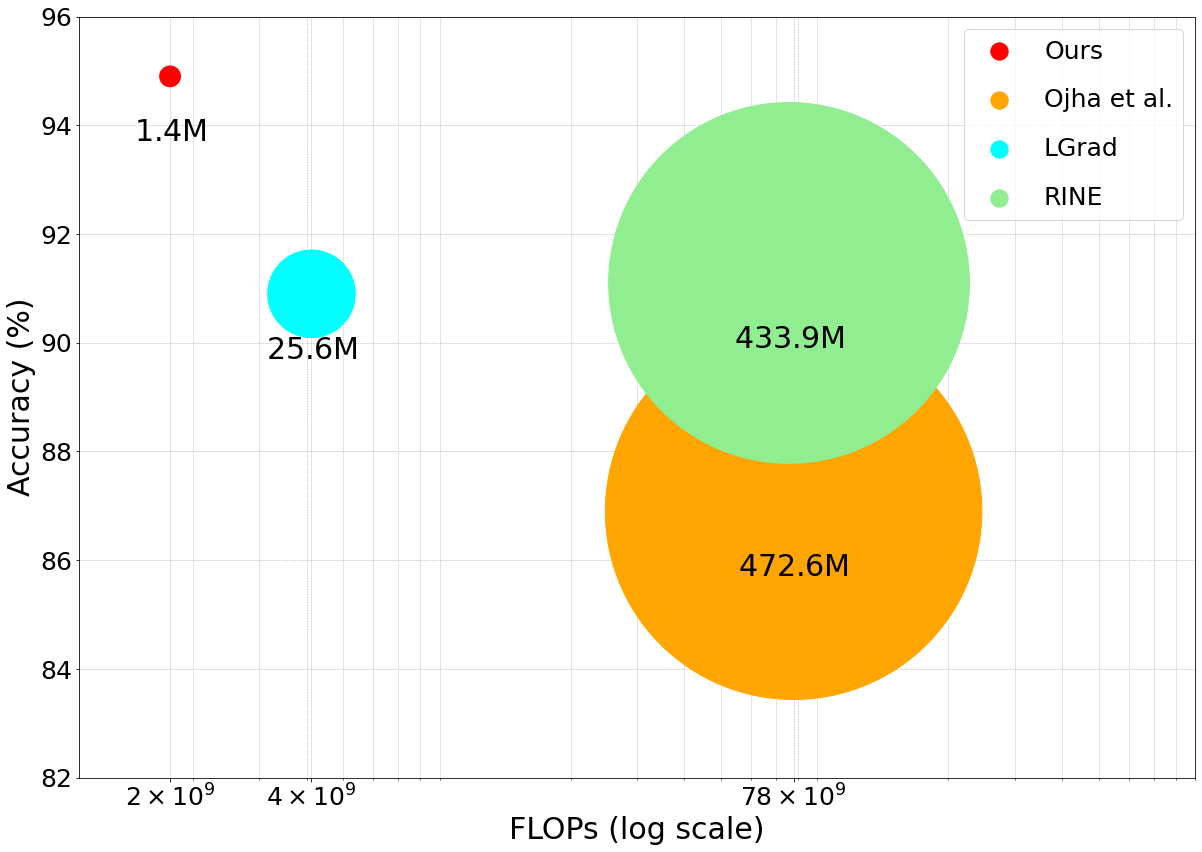
\includegraphics[width=0.7\textwidth]{Images/tease.png}
	%    \fbox{\rule{0pt}{3in} \rule{3in}{0pt}} % Khung ảnh trống
	\caption{Tổng quan hiệu năng và độ chính xác của một số hướng tiếp cận, trên tập dữ liệu Ojha~\cite{Ojha2023TowardsUF}.}
	\label{fig:teaser}
\end{figure}
\subsection{So sánh và đánh giá về độ chính xác}
%\comment{Nhớ thêm chú thích thuật ngữ 'State-of-the-Art'}\\
%
Luận văn thực hiện so sánh độ chính xác của phương pháp đề xuất với 10 phương pháp tiên tiến, bao gồm: 
CNNDetection~\cite{Wang2019CNNGeneratedIA}, 
Frank~\cite{Frank2020LeveragingFA}, 
Durall~\cite{Durall2020WatchYU}, 
Patchfor~\cite{Chai2020WhatMF}, 
F3Net~\cite{Qian2020ThinkingIF}, 
SelfBland~\cite{Shiohara2022DetectingDW}, 
GANDetection~\cite{Mandelli2022DetectingGI}, 
LGrad~\cite{Tan2023LearningOG}, 
Ojha~\cite{Ojha2023TowardsUF}, 
NPR~\cite{Tan2023RethinkingTU}. 
Kết quả thí nghiệm trong các Bảng~\ref{tab:table2}, \ref{tab:table3}, và \ref{tab:table4} cho thấy phương pháp đề xuất vượt trội hơn so với các phương pháp hiện có. 

Trên bộ dữ liệu 9-GAN, ADOF đạt độ chính xác cao nhất là 94.2\%, vượt qua Ojha~\cite{Ojha2023TowardsUF} với chỉ 77.6\% \ref{tab:table2}, và NPR~\cite{Tan2023RethinkingTU} đạt 93.2\% (xem Bảng~\ref{tab:table2}).

Độ chính xác đạt 98.3\% trên tập dữ liệu DiffusionForensics~\cite{Wang2023DIREFD}, cao nhất trong 10 phương pháp, trong khi đó NPR~\cite{Tan2023RethinkingTU} giữ vị trí thứ hai với 95.3\% (xem Bảng~\ref{tab:table3}). Kết quả này cao hơn DIRE~\cite{Wang2023DIREFD} với 97.9\% ngay trên bộ dữ liệu của chính họ, mặc dù mô hình đề xuất trong luận văn được huấn luyện trên Forensynths~\cite{Krizhevsky2012ImageNetCW}, trong khi DIRE được huấn luyện trên DiffusionForensics.

Ngoài ra, độ chính xác cũng trội hơn RINE~\cite{koutlis2024leveraging} và Ojha~\cite{Ojha2023TowardsUF}(91.1\%) (xem Bảng~\ref{tab:table4}). Đáng chú ý, cả hai phương pháp này đều sử dụng mô hình CLIP~\cite{abs-2103-00020} có số lượng tham số rất lớn, yêu cầu nhiều tài nguyên tính toán.

\begin{table}[ht!]%[htbp]
	\centering
	\caption{Kết quả đánh giá trên tập Self-Synthesis 9~GANs~\cite{Tan2023RethinkingTU}.}
	\label{tab:table2}
	\begin{adjustbox}{max width=\textwidth}
		\begin{tabular}{l cc cc cc cc cc cc cc cc cc|cc}
			\toprule
			\vspace{1ex}
			\multirow{2}{*}{{\textbf{Method}}} & \multicolumn{2}{c}{\textbf{AttGAN}} & \multicolumn{2}{c}{\textbf{BEGAN}} & \multicolumn{2}{c}{\textbf{CramerGAN}} & \multicolumn{2}{c}{\textbf{InfoMaxGAN}} & \multicolumn{2}{c}{\textbf{MMDGAN}} & \multicolumn{2}{c}{\textbf{RelGAN}} & \multicolumn{2}{c}{\textbf{S3GAN}} & \multicolumn{2}{c}{\textbf{SNGAN}} & \multicolumn{2}{c|}{\textbf{STGAN}} & \multicolumn{2}{c}{\textbf{Mean}} \\
			\cline{2-21}
			& {\textbf{Acc.}} & {\textbf{A.P.}} & {\textbf{Acc.}} & {\textbf{A.P.}} & {\textbf{Acc.}} & {\textbf{A.P.}} & {\textbf{Acc.}} & {\textbf{A.P.}} & {\textbf{Acc.}} & {\textbf{A.P.}} & {\textbf{Acc.}} & {\textbf{A.P.}} & {\textbf{Acc.}} & {\textbf{A.P.}} & {\textbf{Acc.}} & {\textbf{A.P.}} & {\textbf{Acc.}} & {A.P.} & {\textbf{Acc.}} & {\textbf{A.P.}} \\
			\hline
			CNNDetection~\cite{Wang2019CNNGeneratedIA}  & 51.1 & 83.7 & 50.2 & 44.9 & 81.5 & 97.5 & 71.1 & 94.7  & 72.9 & 94.4 & 53.3 & 82.1 & 55.2 & 66.1 & 62.7 & 90.4 & 63.0 & 92.7 & 62.3 & 82.9 \\
			Frank~\cite{Frank2020LeveragingFA} & 65.0 & 74.4 & 39.4 & 39.9 & 31.0 & 36.0 & 41.1 & 41.0 & 38.4 & 40.5 & 69.2 & 96.2 & 69.7 & 81.9 & 48.4 & 47.9 & 25.4 & 34.0 & 47.5 & 54.7 \\
			Durall~\cite{Durall2020WatchYU} & 39.9 & 38.2 & 48.2 & 30.9 & 60.9 & 67.2 & 50.1 & 51.7 & 59.5 & 65.5 & 80.0 & 88.2 & \textbf{87.3} & 97.0 & 54.8 & 58.9 & 62.1 & 72.5 & 60.3 & 63.3 \\
			Patchfor~\cite{Chai2020WhatMF}  & 68.0 & 92.9 & 97.1 & 100.0 & 97.8 & \textbf{99.9} & 93.6 & 98.2 & 97.9 & \textbf{100.0} & 99.6 & 100.0 & 66.8 & 68.1 & \textbf{97.6} & \textbf{99.8} & 92.7 & 99.8 & 90.1 & 95.4 \\
			F3Net & 85.2 & 94.8 & 87.1 & 97.5 & 89.5 & 99.8 & 67.1 & 83.1 & 73.7 & 99.6 & 98.8 & 100.0 & 65.4 & 70.0 & 51.6 & 93.6 & 60.3 & 99.9 & 75.4 & 93.1 \\
			SelfBland~\cite{Shiohara2022DetectingDW}  & 63.1 & 66.1 & 56.4 & 59.0 & 75.1 & 82.4 & 79.0 & 82.5 & 68.6 & 74.0 & 73.6 & 77.8 & 53.2 & 53.9 & 61.6 & 65.0 & 61.2 & 66.7 & 65.8 & 69.7 \\
			GANDetection~\cite{Mandelli2022DetectingGI} & 57.4 & 75.1 & 67.9 & 100.0 & 67.8 & 99.7 & 67.6 & 92.4 & 67.7 & 99.3 & 60.9 & 86.2 & 69.6 & 83.5 & 66.7 & 90.6 & 69.6 & 97.2 & 66.1 & 91.6 \\
			LGrad~\cite{Tan2023LearningOG}  & 68.6 & 93.8 & 69.9 & 89.2 & 50.3 & 54.0 & 71.1 & 82.0 & 57.5 & 67.3 & 89.1 & 99.1 & 78.5 & 86.0 & 78.0 & 87.4 & 54.8 & 68.0 & 68.6 & 80.8\\
			Ojha~\cite{Ojha2023TowardsUF} & 78.5 & 98.3 & 72.0 & 98.9 & 77.6 & 99.8 & 77.6 & 98.9 & 77.6 & 99.7 & 78.2 & 98.7 & 85.2 & \textbf{98.1} & 77.6 & 98.7 & 74.2 & 97.8 & 77.6 & \textbf{98.8}\\
			NPR~\cite{Tan2023RethinkingTU} &  83.0 & 96.2 & \textbf{99.0} & 99.8 & \textbf{98.7} & 99.0 & \textbf{94.5} & 98.3 & \textbf{98.6} & 99.0 & 99.6 & 100.0 & 79.0 & 80.0 & 88.8 & 97.4 & \textbf{98.0} & \textbf{100.0} & 93.2 & 96.6 \\
			%PatchCraft & 99.7 & 99.99 & 61.1 & 86.0  & 72.4 & 78.4  & 87.5 & 93.3  & 79.8 & 84.3  & 99.5 & 99.9   & 94.0 & 97.9  & 85.1 & 93.2  & 68.6 & 91.3  & 83.1 & 91.6 \\
			\rowcolor{lightgray} {\textbf{ADOF(ours)}} & \textbf{99.5} & \textbf{100.0} & 92.2 & \textbf{100.0} & 96.0 & 99.6 & 94.1 & \textbf{99.1} & 96.0 & 99.7 & \textbf{100.0} & \textbf{100.0} & 77.5 & 86.7 & 94.8 & 99.3 & 97.8 & 99.7 & \textbf{94.2} & 98.2 \\
			\hline
		\end{tabular}
	\end{adjustbox}
\end{table}


\begin{table}[ht!]%[htbp]
	\centering
	\caption{Kết quả đánh giá trên tập DiffusionForensics~\cite{Wang2023DIREFD}.}
	\label{tab:table3}
	\begin{adjustbox}{max width=\textwidth}
		\begin{tabular}{l cc cc cc cc cc cc cc cc|cc}
			\toprule
			%\multirow{2}{*}{\shortstack{Method}} & \multicolumn{2}{c}{\shortstack{ADM}} & \multicolumn{2}{c}{\shortstack{DDPM}} & \multicolumn{2}{c}{\shortstack{IDDPM}} & \multicolumn{2}{c}{\shortstack{LDM}} & \multicolumn{2}{c}{\shortstack{PNDM}} & \multicolumn{2}{c}{\shortstack{VQ-Diffusion}} & \multicolumn{2}{c}{\shortstack{Stable\\Diffusion v1}} & \multicolumn{2}{c}{\shortstack{Stable\\Diffusion v2}} & \multicolumn{2}{c}{\shortstack{Mean}} \\
			\multirow{2}{*}{\shortstack{\textbf{Method}}} & \multicolumn{2}{c}{\shortstack{\textbf{ADM}}} & \multicolumn{2}{c}{\shortstack{\textbf{DDPM}}} & \multicolumn{2}{c}{\shortstack{\textbf{IDDPM}}} & \multicolumn{2}{c}{\shortstack{\textbf{LDM}}} & \multicolumn{2}{c}{\shortstack{\textbf{PNDM}}} & \multicolumn{2}{c}{\shortstack{\textbf{VQ-Diffusion}}} & \multicolumn{2}{c}{\shortstack{\textbf{Stable}\\\textbf{Diffusion v1}}} & \multicolumn{2}{c}{\shortstack{\textbf{Stable}\\\textbf{Diffusion v2}}} & \multicolumn{2}{c}{\shortstack{\textbf{Mean}}} \\
			
			\cline{2-19}
			& \textbf{Acc.} & \textbf{A.P.} & \textbf{Acc.} & \textbf{A.P.} & \textbf{Acc.} & \textbf{A.P.} & \textbf{Acc.} & \textbf{A.P.} & \textbf{Acc.} & \textbf{A.P.} & \textbf{Acc.} & \textbf{A.P.} & \textbf{Acc.} & \textbf{A.P.} & \textbf{Acc.} & \textbf{A.P.} & \textbf{Acc.} & \textbf{A.P.} \\
			
			\hline
			CNNDetection~\cite{Wang2019CNNGeneratedIA}  & 53.9 & 71.8 & 62.7 & 76.6 & 50.2 & 82.7 & 50.4 & 78.7 & 50.8 & 90.3 & 50.0 & 71.0 & 38.0 & 76.7 & 52.0 & 90.3 & 51.0 & 79.8 \\
			Frank~\cite{Frank2020LeveragingFA}  & 58.9 & 65.9 & 37.0 & 27.6 & 51.4 & 65.0 & 51.7 & 48.5 & 44.0 & 38.2 & 51.7 & 66.7 & 32.8 & 52.3 & 40.8 & 37.5 & 46.0 & 50.2 \\
			Durall~\cite{Durall2020WatchYU}  & 39.8 & 42.1 & 52.9 & 49.8 & 55.3 & 56.7 & 43.1 & 39.9 & 44.5 & 47.3 & 38.6 & 38.3 & 39.5 & 56.3 & 62.1 & 55.8 & 47.0 & 48.3 \\
			Patchfor~\cite{Chai2020WhatMF}   & 77.5 & 93.9 & 62.3 & 97.1 & 50.0 & 91.6 & 99.5 & 100.0 & 50.2 & 99.9 & 100.0 & 100.0 & 90.7 & 99.8 & 94.8 & 100.0 & 78.1 & 97.8\\
			F3Net~\cite{Qian2020ThinkingIF} & 80.9 & 96.9 & 84.7 & 99.4 & 74.7 & 98.9 & 100.0 & 100.0 & 72.8 & 99.5 & 100.0 & 100.0 & 73.4 & 97.2 & 99.8 & 100.0 & 85.8 & 99.0 \\
			SelfBland~\cite{Shiohara2022DetectingDW}   & 57.0 & 59.0 & 61.9 & 49.6 & 63.2 & 66.9 & 83.3 & 92.2 & 48.2 & 48.2 & 77.2 & 82.7 & 46.2 & 68.0 & 71.2 & 73.9 & 63.5 & 67.6 \\
			GANDetection~\cite{Mandelli2022DetectingGI}  & 51.1 & 53.1 & 62.3 & 46.4 & 50.2 & 63.0 & 51.6 & 48.1 & 50.6 & 79.0 & 51.1 & 51.2 & 39.8 & 65.6 & 50.1 & 36.9 & 50.8 & 55.4 \\
			LGrad~\cite{Tan2023LearningOG}   & 86.4 & 97.5 & \textbf{99.9} & 100.0 & 66.1 & 92.8 & 99.7 & 100.0 & 69.5 & 98.5 & 96.2 & 100.0 & 90.4 & 99.4 & 97.1 & 100.0 & 88.2 & 98.5 \\
			Ojha~\cite{Ojha2023TowardsUF} & 78.4 & 92.1 & 72.9 & 78.8 & 75.0 & 92.8 & 82.2 & 97.1 & 75.3 & 92.5 & 83.5 & 97.7 & 56.4 & 90.4 & 71.5 & 92.4 & 74.4 & 91.7\\
			NPR~\cite{Tan2023RethinkingTU}  & 88.6 & 98.9 & 99.8 & 100.0 & 91.8 & 99.8 & 100.0 & 100.0 & 91.2 & \textbf{100.0} & 100.0 & 100.0 & 97.4 & 99.8 & 93.8 & 100.0 & 95.3 & 99.8 \\
			\rowcolor{lightgray} {\textbf{ADOF(ours)}} & \textbf{93.5} & \textbf{99.0} & 99.6 & \textbf{100.0} & \textbf{99.2} & \textbf{100.0} & 99.9 & \textbf{100.0} & \textbf{97.4} & 99.9 & 97.1 & 99.8 & \textbf{99.8} & \textbf{100.0} & \textbf{99.9} & \textbf{100.0} & \textbf{98.3} & \textbf{99.8} \\
			
			\bottomrule
		\end{tabular}
	\end{adjustbox}
\end{table}




\begin{table}[ht!]%[htbp]
	\caption{Kết quả đánh giá trên tập Ojha~\cite{Ojha2023TowardsUF}.}
	\label{tab:table4}
	\centering
	\begin{adjustbox}{max width=\textwidth}
		\begin{tabular}{l cc cc cc cc cc cc cc cc|cc}
			\hline
			\multirow{2}{*}{{\textbf{Method}}} & \multicolumn{2}{c}{\textbf{DALLE}} & \multicolumn{2}{c}{$\mathbf{{Glide_{(100\_10)}}}$} & \multicolumn{2}{c}{$\mathbf{{Glide_{(100\_27)}}}$} & \multicolumn{2}{c}{$\mathbf{{Glide_{(50\_27)}}}$} & \multicolumn{2}{c}{\textbf{ADM}} & \multicolumn{2}{c}{$\mathbf{{LDM_{(100)}}}$} & \multicolumn{2}{c}{$\mathbf{{LDM_{(200)}}}$} & \multicolumn{2}{c|}{$\mathbf{{LDM_{(200\_cfg)}}}$} & \multicolumn{2}{c}{\textbf{Mean}} \\
			\cline{2-19}
			& {\textbf{Acc.}} & {\textbf{A.P.}} & {\textbf{Acc.}} & {\textbf{A.P.}} & {\textbf{Acc.}} & {\textbf{A.P.}} & {\textbf{Acc.}} & {\textbf{A.P.}} & {\textbf{Acc.}} & {\textbf{A.P.}} & {\textbf{Acc.}} & {\textbf{A.P.}} & {\textbf{Acc.}} & {\textbf{A.P.}} & {\textbf{Acc.}} & {\textbf{A.P.}} & {\textbf{Acc.}} & {\textbf{A.P.}} \\
			
			\hline
			CNNDetection~\cite{Wang2019CNNGeneratedIA}  & 51.8 & 61.3 & 53.3 & 72.9 & 53.0 & 71.3 & 54.2 & 76.0 & 54.9 & 66.6 & 51.9 & 63.7 & 52.0 & 64.5 & 51.6 & 63.1 & 52.8 & 67.4 \\
			Frank~\cite{Frank2020LeveragingFA}   & 57.0 & 62.5 & 53.6 & 44.3 & 50.4 & 40.8 & 52.0 & 42.3 & 53.4 & 52.5 & 56.6 & 51.3 & 56.4 & 50.9 & 56.5 & 52.1 & 54.5 & 49.6 \\
			Durall~\cite{Durall2020WatchYU}  & 55.9 & 58.0 & 54.9 & 52.3 & 48.9 & 46.9 & 51.7 & 49.9 & 40.6 & 42.3 & 62.0 & 62.6 & 61.7 & 61.7 & 58.4 & 58.5 & 54.3 & 54.0 \\
			Patchfor~\cite{Chai2020WhatMF}   & 79.8 & {99.1} & 87.3 & 99.7 & 82.8 & 99.1 & 84.9 & 98.8 & 74.2 & 81.4 & 95.8 & 99.8 & 95.6 & 99.9 & 94.0 & 99.8 & 86.8 & 97.2 \\
			F3Net~\cite{Qian2020ThinkingIF}  & 71.6 & 79.9 & 88.3 & 95.4 & 87.0 & 94.5 & 88.5 & 95.4 & 69.2 & 70.8 & 74.1 & 84.0 & 73.4 & 83.3 & 80.7 & 89.1 & 79.1 & 86.5 \\
			SelfBland~\cite{Shiohara2022DetectingDW}    & 52.4 & 51.6 & 58.8 & 63.2 & 59.4 & 64.1 & 64.2 & 68.3 & 58.3 & 63.4 & 53.0 & 54.0 & 52.6 & 51.9 & 51.9 & 52.6 & 56.3 & 58.7 \\
			GANDetection~\cite{Mandelli2022DetectingGI}  & 67.2 & 83.0 & 51.2 & 52.6 & 51.1 & 51.9 & 51.7 & 53.5 & 49.6 & 49.0 & 54.7 & 65.8 & 54.9 & 65.9 & 53.8 & 58.9 & 54.3 & 60.1 \\
			LGrad~\cite{Tan2023LearningOG}    & 88.5 & 97.3 & 89.4 & 94.9 & 87.4 & 93.2 & 90.7 & 95.1 & \textbf{86.6} & \textbf{100.0} & 94.8 & 99.2 & 94.2 & 99.1 & 95.9 & 99.2 & 90.9 & 97.2 \\
			Ojha~\cite{Ojha2023TowardsUF}   & 89.5 & 96.8 & 90.1 & 97.0 & 90.7 & 97.2 & 91.1 & 97.4 & 75.7 & 85.1 & 90.5 & 97.0 & 90.2 & 97.1 & 77.3 & 88.6 & 86.9 & 94.5 \\
			NPR~\cite{Tan2023RethinkingTU}   & {94.5} & \textbf{99.5} & 98.2 & 99.8 & 97.8 & 99.7 & 98.2 & 99.8 & 75.8 & 81.0 & \textbf{99.3} & 99.9 & \textbf{99.1} & 99.9 & \textbf{99.0} & 99.8 & \textbf{95.2} & 97.4 \\
			%PatchCraft & 83.3 & 93.0 & 80.1 & 92.0  & 83.4 & 93.9  & 77.6 & 88.7 & 80.9 & 90.5  & 88.9 & 97.7  & 89.3 & 97.9  & 88.1 & 96.9 & 84.0 & 93.8 \\
			RINE~\cite{koutlis2024leveraging}   & \textbf{95.0} & 99.5 & 90.7 & 99.2 & 88.9 & 99.1 & 92.6 & 99.5 & 76.1 & 96.6 & {98.7} & 99.9 & {98.3} & 99.9 & 88.2 & 98.7 & {91.1} & 99.0 \\
			\rowcolor{lightgray}{\textbf{ADOF(ours)}} & 92.1 & 98.3 & \textbf{98.6} & \textbf{100.0} & \textbf{98.7} & \textbf{100.0} & \textbf{98.4} & \textbf{99.9} & 75.9 & 87.6 & 98.8 & \textbf{100.0} & 98.6 & \textbf{99.9} & 98.5 & \textbf{99.9} & 94.9 & \textbf{98.2} \\
			
			\hline
		\end{tabular}
	\end{adjustbox}
\end{table}

%RINE Ojha 4-class
%dalle: 95.0 / 99.5
%glide_100_10: 90.7 / 99.2
%glide_100_27: 88.9 / 99.1
%glide_50_27: 92.6 / 99.5
%guided: 76.1 / 96.6
%ldm_100: 98.7 / 99.9
%ldm_200: 98.3 / 99.9
%ldm_200_cfg: 88.2 / 98.7
%Mean: 91.1 / 99.0
\subsection{So sánh và đánh giá về hiệu năng}
%
%
Để so sánh về hiệu năng, luận văn thực hiện đo lường các tiêu chí về độ phức tạp của mô hình cũng như số lượng phép toán cần thiết cho mỗi dự đoán (chi tiết xem Bảng~\ref{tab:model_performance}). Tất cả được thực hiện trên máy tính có CPU AMD Ryzen 5 5600X 6-Core, GPU NVIDIA RTX A4000, 16 GB bộ nhớ RAM. Hình ảnh đầu vào có kích thước $256 \times 256 \times 3$. Các tiêu chí đánh giá bao gồm:
%
\begin{figure}[ht!]
	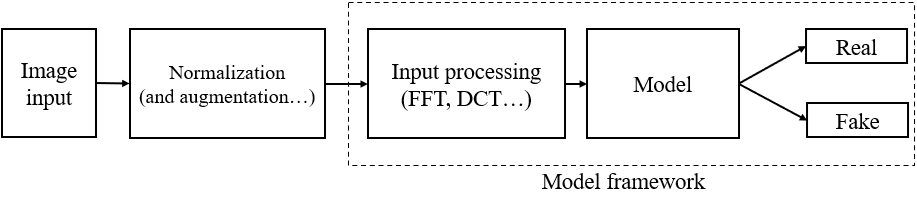
\includegraphics[width=\textwidth]{Images/figure_pine_line_1.png}
	\caption{Quy trình cơ bản của mô hình phát hiện ảnh tạo sinh}	
	\label{figure_pine_line_1}
\end{figure}
%
%
\begin{itemize}
	\item \textbf{Number of Parameters:} Số lượng tham số của mô hình, thể hiện độ phức tạp trong kiến trúc.
	\item \textbf{Input Processing Time:} Đo lường thời gian cần thiết để xử lý hình ảnh trước khi đưa vào mô hình dự đoán, các bước xử lý này thay đổi theo hướng tiếp cận cụ thể (xem Hình.~\ref{figure_pine_line_1}).
	\item \textbf{Inference Time:} Thời gian cần sử dụng cho một dự đoán.
	\item \textbf{FLOPs:} Số lượng phép tính dấu chấm động trong 1 giây, luận văn sử dụng thư viện \texttt{fvcore} để ước tính khối lượng tính toán mà mỗi mô hình cần thực hiện cho một dự đoán.
\end{itemize}
%
%
\begin{table}[h!]
	\centering
	\caption{Tài nguyên sử dụng và hiệu năng của các phương pháp phát hiện hình ảnh tổng hợp, trên tập dữ liệu DiffusionForensics~\cite{Wang2023DIREFD}. Dấu \textsuperscript{$\dagger$} thể hiện phương pháp đã được huấn luyện trên cùng tập dữ liệu.}
	\label{tab:model_performance}
	\begin{adjustbox}{max width=\textwidth}
		\setlength{\tabcolsep}{12pt} % Tăng khoảng cách giữa các cột cho bảng này
		\renewcommand{\arraystretch}{1.1} % Điều chỉnh chỉ cho bảng này
		\begin{tabular}{l c c c c c}
			\toprule
			\multirow{2}{*}{\textbf{Method}} &
			\multirow{2}{*}{\textbf{Parameters}} &
			\multirow{2}{*}{\begin{tabular}[c]{@{}c@{}}\textbf{Processing} \\ \textbf{(ms)}\end{tabular}} &
			\multirow{2}{*}{\begin{tabular}[c]{@{}c@{}}\textbf{Inference Time}\\ \textbf{(ms)}\end{tabular}} &
			\multirow{2}{*}{\textbf{FLOPs}} &
			\multirow{2}{*}{\begin{tabular}[c]{@{}c@{}}\textbf{Means} \\ \textbf{(acc/ap)} \end{tabular}} \\
			&   &   &   &   &    \\ \hline
			LGrad~\cite{Tan2023LearningOG} (2023) & {$25.56 \times 10^6$} & {11.6} & {4.81} & {$4.12 \times 10^9$} & {88.2/98.5}\\ %\hline
			%LNP & {$23.51 \times 10^6$} & {65.6} & -- & {$4.12 \times 10^9$} & {--}\\ %\hline
			DIRE\textsuperscript{$\dagger$}~\cite{Wang2023DIREFD} (2023) & {$25.56 \times 10^6$} & {4,502.7} & {4.81} & {$4.12 \times 10^9$} & {97.9/\textbf{100}}\\ %\hline
			Ojha~\cite{Ojha2023TowardsUF} (2023) & {$427.62 \times 10^6$} & {None} & {29.19} & {$77.83 \times 10^9$} & {74.4/91.7}\\ %\hline
			%PatchCraft~\cite{zhong2024patchcraftexploringtexturepatch} & {$\mathbf{0.12 \times 10^6}$} & {--} & {--} & {$6.70 \times 10^9$} & {84.0/92.7}\\ %\hline
			\rowcolor{lightgray} \textbf{ADOF(ours)} & {\textbf{$1.44 \times 10^6$}} & 0.40 & \textbf{2.43} & {$\mathbf{1.74 \times 10^9}$} & {\textbf{98.3}/99.8}\\ \bottomrule
		\end{tabular}
	\end{adjustbox}
\end{table}








%\chapter{KẾT LUẬN VÀ HƯỚNG PHÁT TRIỂN}

\section{Kết luận}
Luận văn đã đề xuất một bộ lọc đơn giản nhưng hiệu quả, được đặt tên là \textbf{ADOF}, nhằm khai thác các biến thiên mức xám cục bộ giữa các điểm ảnh lân cận. Bằng cách xem hình ảnh như một tín hiệu số rời rạc và áp dụng kỹ thuật sai phân, phương pháp đã loại bỏ các thành phần tần số thấp của tín hiệu — vốn thường mang tính ngữ nghĩa cao nhưng lại không hữu ích trong việc phân biệt giữa ảnh thật và ảnh tạo sinh.

Bộ lọc tập trung vào việc làm nổi bật các dấu vết tinh vi còn lại, từ đó hỗ trợ mô hình học sâu trong việc cải thiện đáng kể cả về độ chính xác và khả năng tổng quát hóa, đồng thời giúp giảm độ phức tạp của mô hình. Kết quả thực nghiệm cho thấy phương pháp ADOF hoạt động hiệu quả ngay cả trên các tập dữ liệu chưa từng được thấy trước đó.

Đặc biệt, khi được tích hợp vào quy trình rút gọn mô hình -- \gls{fbkd}, ADOF vẫn duy trì được lợi ích ban đầu của nó, giúp mô hình \gls{student} đạt hiệu năng gần tương đương với mô hình gốc (\gls{teacher}) nhưng với cấu trúc nhẹ hơn đáng kể. Điều này cho thấy tiềm năng ứng dụng của ADOF trong các hệ thống thực tế yêu cầu tính hiệu quả và khả năng triển khai cao trên thiết bị giới hạn tài nguyên.

\section{Hướng phát triển}
Dựa trên những kết quả khả quan mà bộ lọc ADOF mang lại, một số hướng phát triển tiềm năng trong tương lai bao gồm:

\begin{itemize}
		
	\item \textbf{Mở rộng sang dữ liệu video:} Áp dụng bộ lọc này trong bối cảnh xử lý video -- một loại dữ liệu mà tốc độ và độ chính xác đóng vai trò đặc biệt quan trọng -- nhằm phát hiện kịp thời các nội dung giả mạo trong chuỗi khung hình liên tục.
		
    \item \textbf{Tích hợp vào các \gls{pipeline} phát hiện khác nhau:} Khảo sát hiệu quả của bộ lọc khi được tích hợp như một bước tiền xử lý trong các hệ thống phát hiện hình ảnh tạo sinh sử dụng nhiều kiến trúc khác nhau. Mục tiêu là đánh giá tính tương thích và khả năng giúp mô hình nâng cao hiệu suất trong các kịch bản thực tế đa dạng.
    
    \item \textbf{Mở rộng ứng dụng trong pháp y hình ảnh:} Nghiên cứu áp dụng bộ lọc ADOF vào các kỹ thuật phát hiện thao tác chỉnh sửa ảnh truyền thống như cắt ghép, làm mờ, che giấu chi tiết, hoặc nguỵ trang nội dung.


\end{itemize}
%
%\section*{Hướng phát triển}
%Trong tương lai, hướng nghiên cứu có thể tiếp tục mở rộng theo các phương án sau:
%
%\begin{itemize}
%	\item ...
%\end{itemize}



%\chapter{KẾT LUẬN VÀ HƯỚNG PHÁT TRIỂN}
%\label{Chapter5}
%
%Luận văn đề xuất một bộ lọc đơn giản nhưng hiệu quả, được đặc tên ADOF, nhằm bắt lấy các biến đổi mức xám giữa những điểm ảnh lân cận nhau. Bằng cách coi hình ảnh như một tín hiệu số rời rạc, áp dụng kỹ thuật sai phân cục bộ, phương pháp này loại bỏ các thành phần trung bình của tín hiệu—những thành phần mang nhiều thông tin ngữ nghĩa, nhưng lại ít hữu ích trong việc phân biệt giữa hình ảnh thật và hình ảnh tổng hợp. Bộ lọc tập trung vào việc trích lọc các dấu vết tinh vi, để cung cấp cho mô hình phân loại.
%
%Kết quả thử nghiệm cho thấy phương pháp không chỉ giảm đáng kể độ phức tạp của mô hình mà còn cải thiện cả độ chính xác lẫn khả năng tổng quát, ngay cả trên các dữ liệu chưa từng được thấy trước đó.

%Ngoài ra, chúng tôi nhận thấy tiềm năng mở rộng nghiên cứu này sang các bài toán pháp y khác, như phát hiện thao tác hình ảnh, ghép nối, mở rộng ảnh và nhận diện ảnh ngụy trang. Chúng tôi dự định tiếp tục khám phá ứng dụng của phương pháp này trong các lĩnh vực đó để nâng cao hơn nữa hiệu quả trong phân tích pháp y.

% Công trình của tác giả
\addcontentsline{toc}{chapter}{Danh mục công trình của tác giả}
\chapter*{Danh mục công trình của tác giả}
\label{publish}

\begin{enumerate}
\item Tên bài báo

\end{enumerate}

% In tài liệu tham khảo
%\addcontentsline{toc}{chapter}{Tài liệu tham khảo}
%\printbibheading[title={Tài liệu tham khảo}]

%\printbibliography[heading=subbibliography, title={Tiếng Việt}, keyword=Viet, resetnumbers=true]

%\DeclareNameAlias{sortname}{family-given}
%\DeclareNameAlias{default}{family-given}

\printbibliography[heading=subbibliography, title={Tiếng Anh}, notkeyword=Viet, resetnumbers=1] 
% Chú ý: phải gán lại resetnumbers=số tài liệu tham khảo tiếng Việt + 1

% Phần phụ lục
%\appendix

\chapter{Ngữ pháp tiếng Việt}
\label{Appendix1}

Đây là phụ lục.
%\chapter{Ngữ pháp tiếng Nôm}
\label{Appendix2}

Đây là phụ lục 2.
%\appendix

\chapter{Các Bảng Dữ Liệu Mở Rộng}
\label{app:tables}

\begin{table}[ht]
	\centering
	\caption{Cấu trúc tập dữ liệu DiffusionForensics~\cite{Wang2023DIREFD}.}
	\label{tab:diffusionforensics_dataset}
	\begin{adjustbox}{max width=\textwidth}
	%\resizebox{1.0\linewidth}{!}{
		\begin{tabular}{lclc}
			\hline
			\multirow{2}{*}{\textbf{Image Source}} & \textbf{Denoising} & \multirow{2}{*}{\textbf{Generator}} & \textbf{\# of images} \\ 
			& \textbf{Condition} & & \textbf{(real/generated)} \\ 
			\hline
			& \multirow{4}{*}{Unconditional} &ADM~\cite{dhariwal2021diffusion} & 42k/42k \\
			& & DDPM~\cite{Ho2020DenoisingDP} & 42k/42k \\
			& & iDDPM~\cite{Nichol2021ImprovedDD} & 42k/42k \\
			LSUN& & PNDM~\cite{Liu2022PseudoNM} & 42k/42k \\ 
			\cline{2-4}
			-Bedroom~\cite{Yu2015LSUNCO} & \multirow{4}{*}{Text2Image} &LDM~\cite{Rombach2021HighResolutionIS} & 1k/1k \\
			& & SD-v1~\cite{Rombach2021HighResolutionIS} & 1k/1k \\
			& & SD-v2~\cite{Rombach2021HighResolutionIS} & 1k/1k \\
			& & VQ-Diffusion~\cite{Gu2021VectorQD} & 1k/1k \\ \hline
			\multirow{2}{*}{ImageNet~\cite{5206848}} & Conditional & ADM~\cite{dhariwal2021diffusion} & 50k/50k \\  \cline{2-4}
			& Text2Image & SD-v1~\cite{Rombach2021HighResolutionIS} & 10k/10k \\
			\hline
		\end{tabular}
	%}
	\end{adjustbox}
	%\vspace{-.5em}
	%\vspace{-1em}
\end{table}
%
%
%
%



%\appendix

\chapter{Các Bảng Dữ Liệu Mở Rộng}
\label{app:tables}

\begin{table}[ht]
	\centering
	\caption{Cấu trúc tập dữ liệu DiffusionForensics~\cite{Wang2023DIREFD}.}
	\label{tab:diffusionforensics_dataset}
	\begin{adjustbox}{max width=\textwidth}
	%\resizebox{1.0\linewidth}{!}{
		\begin{tabular}{lclc}
			\hline
			\multirow{2}{*}{\textbf{Image Source}} & \textbf{Denoising} & \multirow{2}{*}{\textbf{Generator}} & \textbf{\# of images} \\ 
			& \textbf{Condition} & & \textbf{(real/generated)} \\ 
			\hline
			& \multirow{4}{*}{Unconditional} &ADM~\cite{dhariwal2021diffusion} & 42k/42k \\
			& & DDPM~\cite{Ho2020DenoisingDP} & 42k/42k \\
			& & iDDPM~\cite{Nichol2021ImprovedDD} & 42k/42k \\
			LSUN& & PNDM~\cite{Liu2022PseudoNM} & 42k/42k \\ 
			\cline{2-4}
			-Bedroom~\cite{Yu2015LSUNCO} & \multirow{4}{*}{Text2Image} &LDM~\cite{Rombach2021HighResolutionIS} & 1k/1k \\
			& & SD-v1~\cite{Rombach2021HighResolutionIS} & 1k/1k \\
			& & SD-v2~\cite{Rombach2021HighResolutionIS} & 1k/1k \\
			& & VQ-Diffusion~\cite{Gu2021VectorQD} & 1k/1k \\ \hline
			\multirow{2}{*}{ImageNet~\cite{5206848}} & Conditional & ADM~\cite{dhariwal2021diffusion} & 50k/50k \\  \cline{2-4}
			& Text2Image & SD-v1~\cite{Rombach2021HighResolutionIS} & 10k/10k \\
			\hline
		\end{tabular}
	%}
	\end{adjustbox}
	%\vspace{-.5em}
	%\vspace{-1em}
\end{table}
%
%
%
%


\end{document} 